% 文章クラス:1段組のA4報告書(和文)
\documentclass[a4j,11pt]{jreport}
\usepackage{amssymb}
\usepackage{multirow} 
\usepackage{midpage}
\usepackage{float}

% 文字のフォント指定
\usepackage{mathptmx}
\usepackage{newtxtext,newtxmath}
\usepackage{subcaption}
\renewcommand{\bfdefault}{bx} % 太字の代替フォントを設定
% \usepackage{titlesec}
% \titleformat*{\section}{\fontsize{12pt}{10pt}\selectfont\bf}
% \titleformat*{\subsection}{\fontsize{10pt}{10pt}\selectfont\bf}

\usepackage{titlesec}
\titleformat*{\section}{\fontsize{14pt}{0pt}\selectfont\bf}
\titleformat*{\subsection}{\fontsize{12pt}{0pt}\selectfont\bf}

\usepackage{setspace}
\usepackage{otf}%はしご高用
\setstretch{1.2}


%ヘッダーの設定
% \usepackage{fancyhdr}
% \usepackage{otf}
%  \pagestyle{fancy}
%     \lhead{\fontsize{10pt}{0pt}\selectfont{\ajRoman{2}}}
%      \chead{}
%     \rhead{}
%数式の設定%
\usepackage{amsmath}
%表のページ跨がせるよう%
\usepackage{longtable}
\usepackage{array}

\usepackage{comment}

% 余白の設定(上下左右:2cm)
\usepackage[margin=30truemm]{geometry}

% 図と表の設定
\usepackage[dvipdfmx]{graphicx}
\renewcommand{\figurename}{Fig. }
\renewcommand{\tablename}{Table}
\setlength\intextsep{10pt} % 図の余白
\setlength\textfloatsep{10pt} % 図の余白
\usepackage{here}

%tableやfigure内で図や表を出すためのコマンド
\makeatletter
\newcommand{\figcaption}[1]{\def\@captype{figure}\caption{#1}}
\newcommand{\tblcaption}[1]{\def\@captype{table}\caption{#1}}
\makeatother

% 追加パッケージ
\usepackage{comment}
\usepackage{subcaption}
\usepackage{url}
\usepackage{multicol}
\usepackage{CJKutf8}
\usepackage[dvipdfmx]{hyperref}
\usepackage{pxjahyper}
\usepackage{otf}
\usepackage{cleveref}
\crefname{figure}{Fig.}{Figs.}
\crefname{table}{Tab.}{Tabs.}
\usepackage{bm}
\usepackage{booktabs}
\usepackage{multirow}
\usepackage{siunitx}
\usepackage{minted}

% ドキュメント開始
\begin{document}
% ~~~表紙~~~
\begin{titlepage}
    \begin{center}
        \fontsize{16.060pt}{24.090pt}\selectfont{修士論文}\\
        \vspace{10.5pt}
        \fontsize{16.060pt}{24.090pt}\selectfont{意味的な画像概念のDNN学習過程における汎化性能について}\\
        \vspace{10.5pt}
        \fontsize{12.045pt}{18.067pt}\selectfont{On generalization performance under DNN learning process of semantic image concepts}\\
        \vspace{10.5pt}
        \fontsize{12.045pt}{18.067pt}\selectfont{\quad}\\
        \vspace{10.5pt}
        \fontsize{12.045pt}{18.067pt}\selectfont{\quad}\\
        \vspace{10.5pt}
        \fontsize{12.045pt}{18.067pt}\selectfont{\quad}\\
        \vspace{10.5pt}
        \fontsize{12.045pt}{18.067pt}\selectfont{\quad}\\
        \vspace{10.5pt}
        \fontsize{12.045pt}{18.067pt}\selectfont{\quad}\\
        \vspace{10.5pt}
        \fontsize{12.045pt}{18.067pt}\selectfont{\quad}\\
        \vspace{10.5pt}
        \fontsize{12.045pt}{18.067pt}\selectfont{\quad}\\
        \vspace{10.5pt}
        \fontsize{12.045pt}{18.067pt}\selectfont{\quad}\\
        \vspace{10.5pt}
        \fontsize{12.045pt}{18.067pt}\selectfont{\quad}\\
        \vspace{10.5pt}
        \fontsize{16.060pt}{24.090pt}\selectfont{\quad}\\
        \vspace{10.5pt}
        \fontsize{16.060pt}{24.090pt}\selectfont{東京電機大学大学院 システムデザイン工学研究科}\\
        \vspace{10.5pt}
        \fontsize{16.060pt}{24.090pt}\selectfont{情報システム工学専攻 修士課程}\\
        \vspace{10.5pt}
        \fontsize{16.060pt}{24.090pt}\selectfont{23AMJ03 岩瀬 俊}\\
        \vspace{10.5pt}
        \fontsize{16.060pt}{24.090pt}\selectfont{研究指導教員 \quad 教授 前田 英作}\\
        \vspace{10.5pt}
    \end{center}
\end{titlepage}

% 文章開始


\chapter*{要旨}
深層ニューラルネットワーク(DNN)を用いたエンドツーエンド学習は,コンピュータビジョン(CV)および自然言語処理(NLP)の諸タスクにおいて高い性能を実証している.しかしながら,分散表現に依存するDNNの解釈可能性は依然として限定的であり,ブラックボックスとして扱われることが多い.この透明性の欠如により,DNNが何を,いつ,どのように学習するのかという深層学習のメカニズムに対する深い理解が妨げられている.
複雑な画像認識タスクは一般的に,複数の意味的な画像概念を並行して学習することを伴い,異なる特徴が様々な時間スケールで学習される.従来研究では形状やテクスチャ特徴の学習が分析されてきたが,これらの概念は通常,与えられたデータセットに基づいて帰納的に定義されており,体系的な分析には制限があった.信頼性の高い分析を行うためには,適切かつ制御可能な難易度レベルと,それらを支持するための十分なデータを有する学習タスクの確立が不可欠である.
これらの課題に対し,本研究では「数字」と「色」という2つの解釈可能な概念に着目し,サンプル間に固有のノイズを含むEMNIST Digitsデータセットに色情報を付加することで,100クラスの分類タスクを構築した.その上で,標準的な条件下および追加的なラベルノイズ存在下におけるDNN学習プロセスの分析を実施した.
本研究の結果より,各概念の獲得難度に応じて学習のタイミングが異なること,また異なる概念の学習間に相互作用が存在することが明らかとなった.これらの知見は,深層学習における画像概念の学習プロセスに関する示唆を与えるものであり,画像ベースのタスクを超えた応用可能性を有するとともに,深層学習のダイナミクスの包括的な理解に寄与するものである.
\newpage

\chapter*{Abstract}

End-to-end learning using deep neural networks (DNNs) has demonstrated high performance across various computer vision (CV) and natural language processing (NLP) tasks. However, the interpretability of DNNs, which rely on distributed representations, remains limited, often rendering them as black boxes. This lack of transparency prevents a deeper understanding of the mechanics of deep learning, specifically regarding what, when, and how DNNs learn.
In contrast, complex image recognition tasks generally involve learning multiple semantic image concepts in parallel, with different features learned at varying time scales. While previous studies have analyzed the learning of shape and texture features, these concepts are typically defined inductively based on the given dataset, limiting systematic analysis.
For reliable analysis, it's crucial to establish learning tasks with appropriate, controllable difficulty levels and sufficient data to support them. To address these needs, we focused on two interpretable concepts—"numbers" and "colors"—and developed a classification task with 100 classes by adding color information to the EMNIST Digits dataset, which includes inherent noise across samples. We then analyzed the DNN learning process under standard conditions and with additional label noise.
Our results reveal that the timing of learning differs depending on the difficulty of acquiring each concept and that there is an interaction between learning different concepts. These findings offer insights into the learning process of image concepts in deep learning, with potential applications beyond image-based tasks, contributing to a broader understanding of deep learning dynamics.

\newpage

\tableofcontents
\newpage
\listoffigures
\newpage
\listoftables
\newpage

\chapter{序論}
深層ニューラルネットワーク(DNN)は,画像認識や自然言語処理など,幅広い分野において著しい性能向上を遂げてきた.特に,ImageNetチャレンジにおける成功を契機に,DNNは視覚的タスクにおいて人間の能力を凌駕する成果を示している\cite{ILSVRC15}.しかし,その性能の背後にある内部表現の形成メカニズムは未だ十分に解明されておらず,その「ブラックボックス」的な性質は重要な研究課題として残されている.モデルの信頼性や透明性を高めるためには,学習プロセスにおける視覚的特徴の獲得メカニズムを明らかにする必要がある.

本研究は,DNNの視覚的特徴の学習プロセスにおいて,特徴獲得の順序や相互作用のメカニズムを明らかにすることを目的とする.特に,学習過程における内部表現の動的変化を系統的に分析するため,新しい実験的枠組みを構築する.視覚的特徴として「数字」と「色」に注目し,データセットを制御することで,学習過程を観察可能な環境を整備する.

本研究では,EMNIST Digitsデータセットに色情報を付加し,視覚的特徴の学習ダイナミクスを解析するための制御可能なデータセットを構築する.これにより,視覚的特徴の学習順序,獲得速度,および特徴間の相互作用を詳細に分析する.学習過程の評価には,モデルの精度を色や数字のみのエラー率に分解し,概念ごとの精度を観察する.
% ,特徴マップの可視化\cite{DBLP:conf/cvpr/ZeilerF14},内部表現のクラスタリング結果など,多角的な評価指標を用いる.

本研究の貢献は以下の3点に要約される.第一に,DNNの学習プロセスを解析するための制御可能な実験環境を構築した.第二に,異なる視覚的特徴の学習順序および相互作用を定量的に評価し,特徴獲得メカニズムを明らかにした.第三に,学習環境におけるノイズの影響を詳細に調査し,モデルのロバスト性と学習効率に関する重要な知見を得た\cite{DBLP:conf/icml/BahdanauCB14}.

これらの成果は,深層学習における内部表現の理解を深めるとともに,効率的かつ解釈可能な学習アルゴリズムの設計に向けた新たな指針を提供するものである.
\newpage
% \begin{figure}[t]
% \centering
% 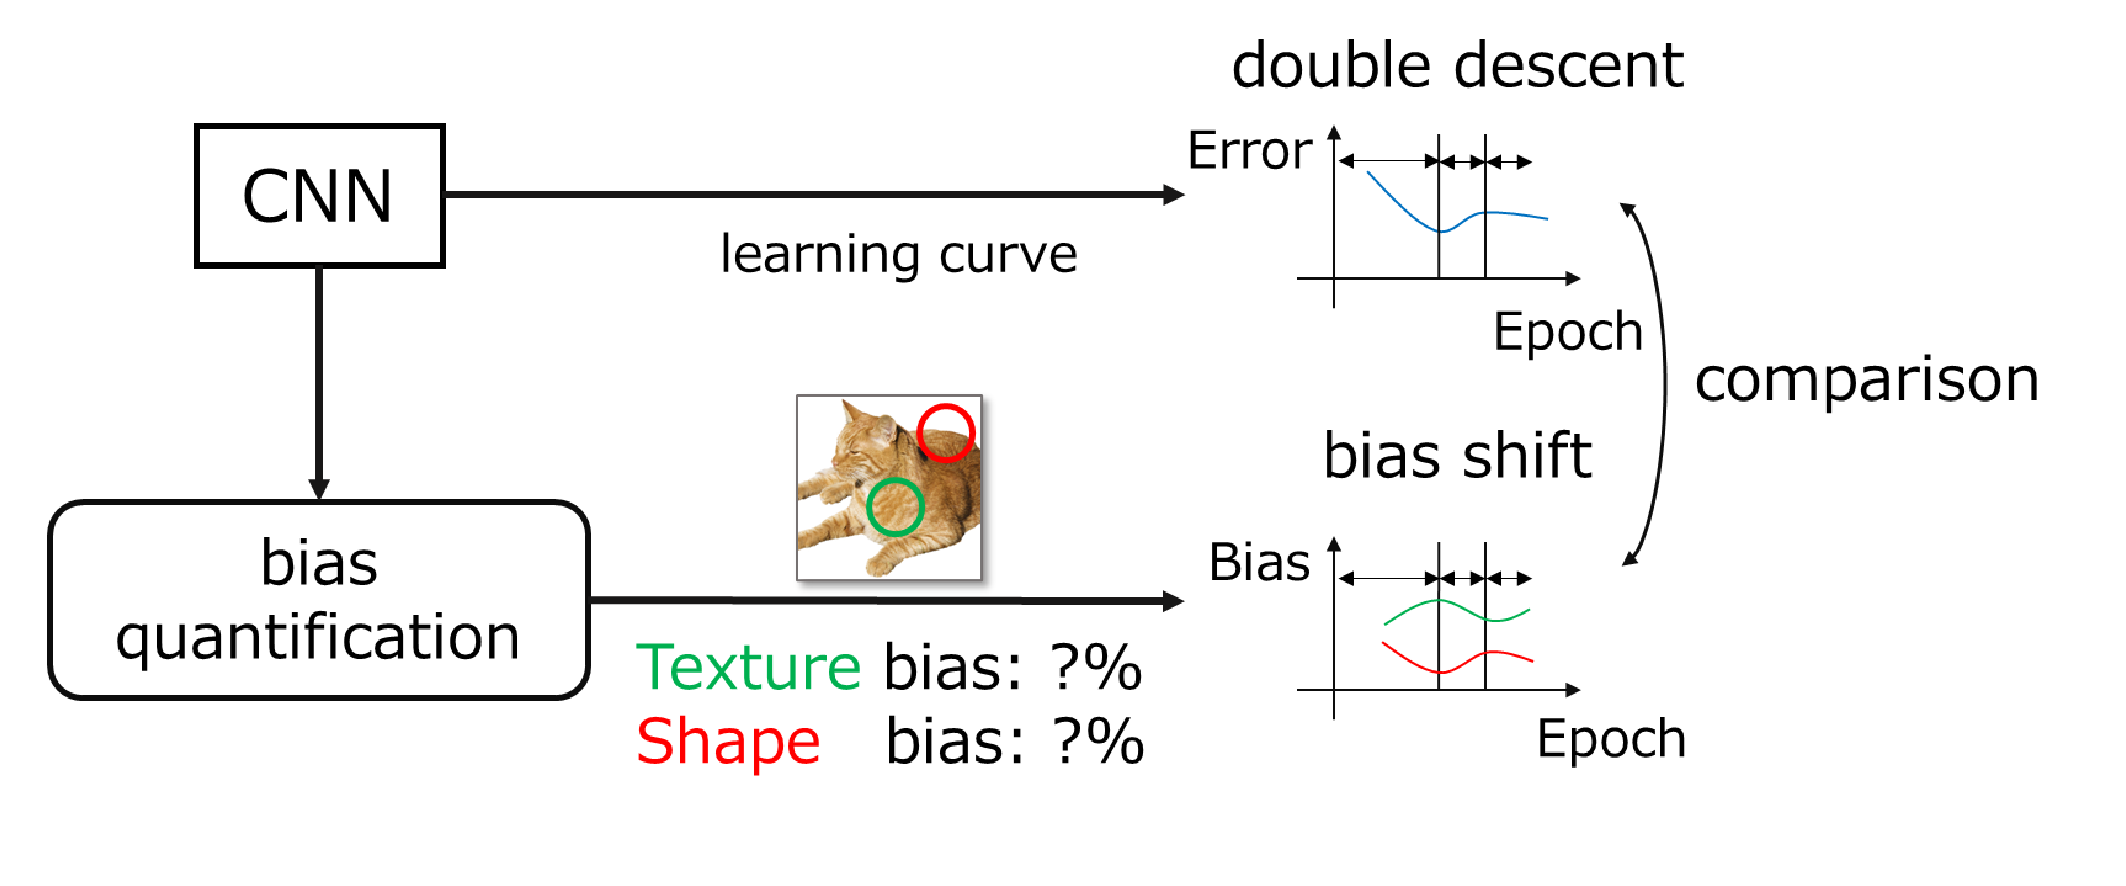
\includegraphics[width=1\columnwidth]{fig/fig1.pdf}
% \vspace{-40pt}
% \caption[ Flow of the analysis process comparing double descent with the learning process of image features.]{
% % 本稿で紹介する解析プロセスの流れ.我々は畳み込みニューラルネットワーク(CNN)を採用し,二重降下条件下で多様な画像認識タスクを訓練した.形状/テクスチャのバイアスとテストエラーの時間的変化を監視し,形状やテクスチャを解釈するモデルの能力を評価すると同時に,それらの相関関係を探った.
% %  Flow of the analysis process comparing double descent with the learning process of image features. We employed convolutional neural networks (CNNs) to train diverse image recognition tasks under double descent conditions. We monitored the temporal evolution of the shape/texture biases and test errors metrics assessing the capacity of the model to interpret shapes and textures while also exploring their correlation.
% }
% \label{fig:fig2}
% \end{figure}

\section{論文構成}
第1章「序論」では,深層学習の急速な発展とその多岐にわたる応用分野について概観し,特に画像認識分野における性能向上とその背景にある主要な技術的進展について述べた.さらに,深層ニューラルネットワーク(DNN)の高い性能を支える内部表現の獲得メカニズムに関する既存の理論的枠組みと,経験的に観測される挙動との間に見られるギャップを指摘し,本研究の対象とする課題の明確化を行った.最後に,DNNの学習プロセスにおける視覚的特徴の獲得順序や相互作用の解明が,モデルの透明性向上や学習効率の改善に寄与することを示し,本研究の目的と貢献点を述べた.\par
第2章「先行研究」では,深層学習における視覚的特徴の獲得の研究がどのように進展してきたかを概観し,特に,画像認識における形状とテクスチャの重要性に関する先行研究を紹介する.さらに,深層学習における重要な経験的に知られる二重降下現象に関する最近の研究成果を紹介し,深層学習の学習プロセスにおける特徴獲得のメカニズムに関する理論的知見と実験的結果を紹介する.\par
第3章「」では,深層学習における,視覚的特徴の獲得メカニズムを紐解くための実験設定を提案し,その設定の理由と目的と述べる.\par
第4章「実験」では,第4章に基づいて行った検証結果,各種パラメータが与える実験結果への影響について検証する.\par
第5章「考察」では,実験結果についての考察を行う.\par
第6章「結論」では,本研究を総括する.\par
第7章「今後の展望」では,本研究で得られた知見から今後の方向性を示す.\par
\newpage 
    
\chapter{先行研究}
\section{深層学習}
一般に,機械学習で使用されるモデルは決定木,サポートベクターマシン(SVM),ニューラルネットワークなどが存在する.決定木は得られた予測に対して,どの説明変数が影響したのかの判断が容易であり,説明可能性が高いことで知られている.
一方で,ニューラルネットワークは,パーセプトロンを筆頭に,層の増加やネットワークの複雑化が図られてきた.黎明期においては,非線形な問題をとけるように知見が盛り込まれたSVMや,生物が持つ視覚野の知見から提案されたネオコグニトロンなどの画期的な手法が提案されてきた.その中でも,ネオコグニトロンに端を発する,畳み込みニューラルネットワーク(CNN)は,LeNet\cite{LeNet}により,誤差逆伝播法が導入され,2010年代以降には,AlexNet\cite{AlexNet},VGGNet\cite{VGGNet},ResNet\cite{ResNet},と急速に進化を遂げてきた.
このような深層化されたニューラルネットワークは興味深い性質や振る舞いを示す.しかし,そのような性質がどのような機序によって引き起こされるかについての完全な合意はとられていない.

\section{二重降下現象}
機械学習において,モデルの性能はモデルの複雑性(例えば,パラメータ数)と深い関係があり,モデルのパラメータ数が不足することによるアンダーフィッティング(Underfitting)\cite{underfitting}や,過剰なパラメータによるオーバーフィッティング(Overfitting)\cite{overfitting}などの現象が知られている.モデルの複雑性が増すにつれて,初めは性能が向上し(アンダーフィッティングを克服),その後過剰な複雑性により性能が低下するとされていた.これはU字型のカーブ,いわゆるバイアス-バリアンス トレードオフ\cite{Rajnarayan2010}として知られている.

ところが近年発見されたDouble Descent\cite{Belkin_2019}と呼ばれている現象は,モデルの複雑性がさらに増すと,性能が再び向上する.つまり,最初のU字型のカーブ(アンダーフィッティングからオーバーフィッティングへの移行)の後,さらに複雑性が増加すると,新たな性能向上のフェーズが現れるのである.過剰パラメータを持つディープニューラルネットワークが,理論的にはオーバーフィッティングを起こすべきなのに,実際には優れた汎化性能を示す場合がある\cite{ResNet,ViT}.

このDouble Descentは,Belkinら\cite{Belkin_2019}によって決定木や二層のニューラルネットワークで確認され,その後,Nakkiranら\cite{nakkiran2021deep}が,ディープニューラルネットワーク(DNN)においても観察されること,学習エポック数の増加に対してもDouble Descentが起こることを示した.さらに,パラメータの枝刈りによるスパース性の増加に対してもDouble Descentが起こることが報告されている\cite{He}.パラメータ数,学習エポック数,スパース性の増加に伴って観察されるDouble Descentは,それぞれ,Model-wise Double Descent,Epoch-wise Double Descent,Sparse Double Descent と呼ばれている\cite{nakkiran2021deep,He}.

\section{画像認識における形状・テクスチャ}
Geirhosらは,ImageNetで学習したCNNが,分類のために特に画像のテクスチャを重視することを示した~\cite{Geirhos}.彼らは,相反する形状とテクスチャ情報を持つ画像をCNNに入力し,出力が形状ベースのラベルとテクスチャベースのラベルのどちらに一致するかをチェックした.この結果に基づいて,CNNが認識において形状とテクスチャのどちらを優先するかを分析した.一方,Islamらは,ニューロンの潜在表現に基づくモデルにおいて,形状とテクスチャのどちらを重視するかを定量的に判断する方法を提案した~\cite{Islam}.この方法によって,CNNがどの特徴に偏重するのかを定量的に分析することができる.さらに,Geらは人間の視覚系のモデル化を試み,Human Vision System (HVS)を開発した.HVSは,画像分類時にどの特徴(形状,テクスチャ,色など)が最も重要な役割を果たすかを定量的に評価可能である\cite{Ge}.

\section{画像認識における二重降下現象と形状・テクスチャバイアスの関係}

\begin{figure}[t]
    \centering
    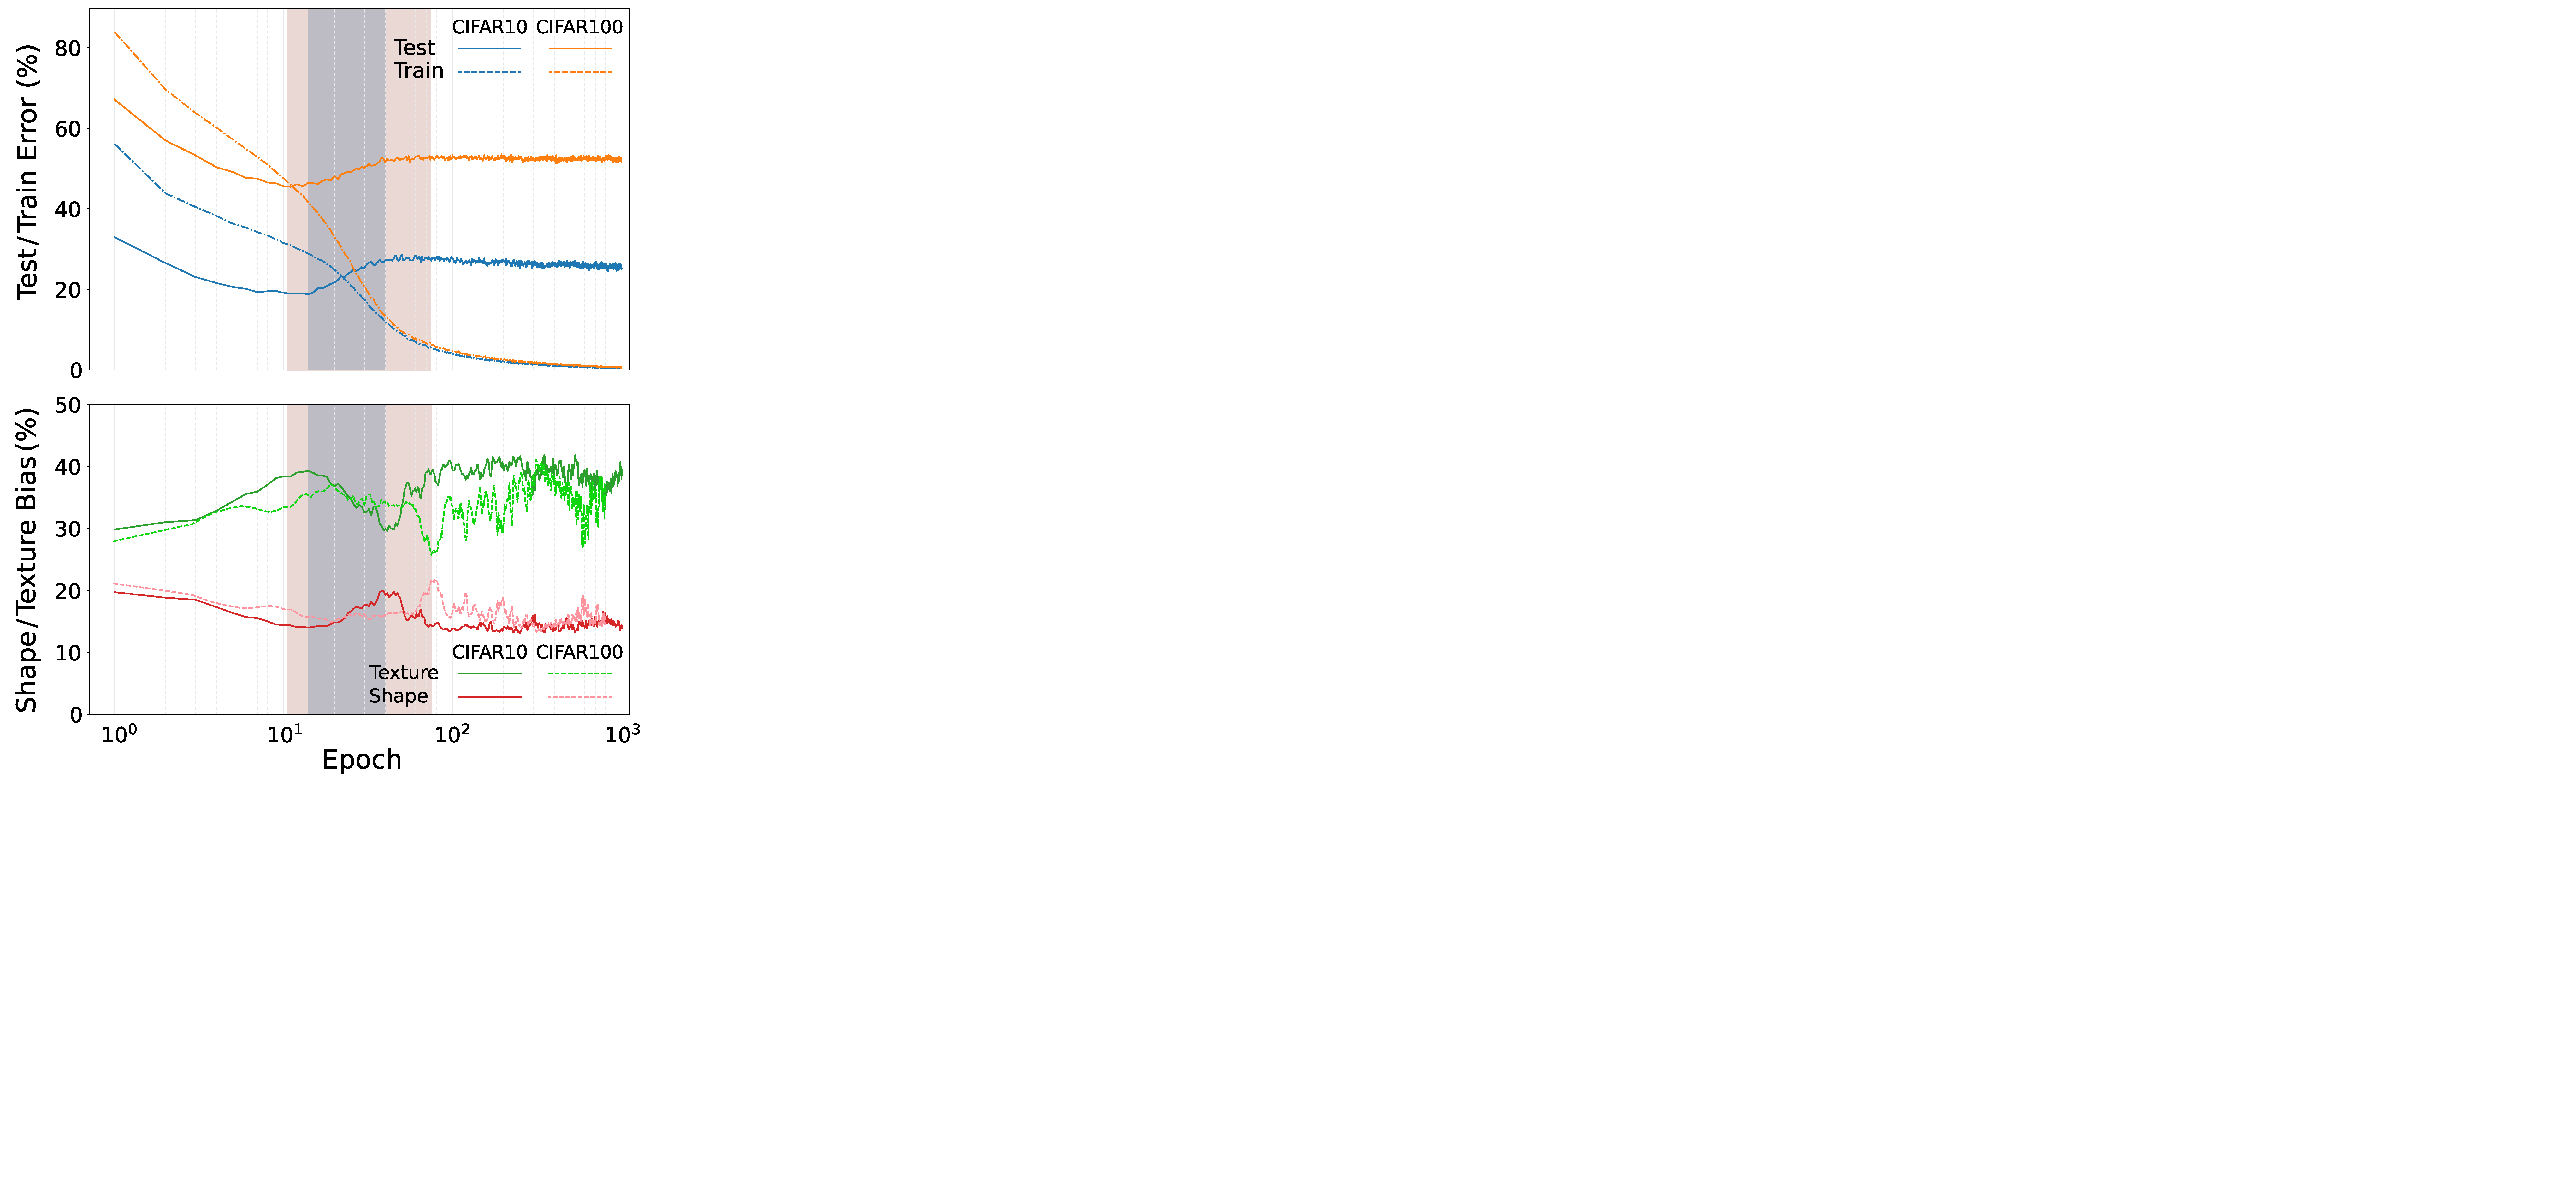
\includegraphics[width=\linewidth]{fig/iwaseICPR.pdf}
    \caption[ResNet18の学習過程における二重降下現象と形状・テクスチャバイアスの変化の同期性.]{ResNet18の学習過程における二重降下現象と形状・テクスチャバイアスの変化の同期性.ImageNetで事前学習済みのResNet18を使用し,CIFAR-10とCIFAR-100の学習を行った際のテストエラー率.また,それぞれのエポックでのモデルにおける形状・テクスチャバイアスを計算した結果.
    二重降下現象を3つのフェーズに分けた際に,第1フェーズでは,テストエラー率が減少するときにはテキスチャバイアスが強くなる.次に過学習のタイミングで形状バイアスが強くなり,再度はエラー率が下がるときテクスチャバイアスを強くするように戻る.}
    \label{fig:iwaseICPR}
\end{figure}
\UTF{9AD9}橋らの研究\cite{DD_STB}は,画像認識タスクにおける二重降下現象と,CNNの形状バイアスおよびテクスチャバイアスの変化の関連性を示唆した.この研究では,二重降下現象と形状・テクスチャバイアスの変化のタイミングに相関が見られ,テスト誤り率が上昇から下降に転じるタイミングと,形状バイアスが増加し始めるタイミングが一致することが示された.
また,事前学習の有無による学習過程の違いも観測された.事前学習ありのモデルでは初期からテクスチャバイアスが高く,学習が進むと形状バイアスが増加する傾向が見られた.一方,事前学習なしのモデルでは学習初期は形状バイアスが高く,その後テクスチャバイアスが増加する傾向が確認された.

岩瀬らの研究~\cite{icpr2024iwase}では,さらに形状・テクスチャバイアスと二重降下現象に関する同期性を様々な角度から検証している.この研究では,CIFAR-10とResNet18の組み合わせ以外の条件下で同期性が確認されたほか,どの層が要因となり,同期性が起こっているのかが明らかとなった.
これらの知見は,画像認識モデルの学習ダイナミクスと二重降下現象の関係性に新たな洞察を提供している.
この同期性を図\ref{fig:iwaseICPR}に示す.
これまでの研究では,CNNの学習過程における形状とテクスチャという特徴の獲得と二重降下現象の関係について研究されてきた.そこで,本研究では形状とテクスチャではなく,色と数字という概念を設定し,2つの学習過程における概念獲得の過程の観測した.
\newpage

\chapter{視覚的特徴の獲得を分析するためのデータセット}
\label{chap:experiment_settings}
本章では,深層学習における,視覚的特徴の獲得メカニズムを紐解くためのデータセットを提案し,その設定の理由と目的と述べる.
これまでの研究では,CNNの学習過程における形状とテクスチャという特徴の獲得と二重降下現象の関係について研究されてきた.
しかし,本研究では形状とテクスチャではなく,色と数字という概念を設定し,2つの学習過程における概念獲得の過程の観測した.

\section{提案データセットの背景}
従来のCNNの研究では,形状バイアスとテクスチャバイアスの学習過程に焦点が当てられてきた.特に,Islamらの研究では,形状とテクスチャを概念として設定して,
CNNモデルの形状・テクスチャバイアスを定量的に計算する手法を提案している.Esserらが提案した定量的に計算する際に使用するデータセット例を以下に示す.

% ここにエッサーのデータセット例を入れる
% \begin{figure}
%     \centering
%     \includegraphics[width=0.8\linewidth]{fig/esserset.pdf}
%     \caption{Esserらの提案した形状・テクスチャバイアスの計算手法.}
%     \label{fig:esserset}
% \end{figure}


また,\UTF{9AD9}橋らの研究により,二重降下現象と形状・テクスチャバイアスの変化のタイミングに相関があることが示されている.
しかし,形状やテクスチャという概念は,データセットから帰納的に定められるものであり,正確に定義することが難しく,より詳細な分析を行うことが困難である.
また,CNNが獲得する視覚的特徴は形状やテクスチャに限らず,より基本的な概念,例えば色や数字といった要素も重要な学習対象となる.
これらの基本的な概念の獲得過程を理解することは,CNNの学習メカニズムの解明に新たな知見をもたらす可能性がある.
そこで,今回の提案するデータセットに関しては,目的である学習過程の概念獲得の分析ということを考え,新たに作成したデータセットを作成するうえで3つの条件を
設定した.

\begin{itemize}
    \item 直感的な概念
    \item 2つの概念が独立
    \item 難易度の操作が可能
\end{itemize}

それぞれの条件を設定した理由について以下に述べる.

\subsection{直感的な概念}
形状やテクスチャの概念は,人間が直感的に理解できる概念であるため,これらの概念を用いた研究が多く行われてきた.
しかし,形状やテクスチャといった概念は,データセットから帰納的に定められるものであり,正確に定義することが難しい.
そのため,より直感的な概念を設定することで,より詳細な分析を行うことが可能となる.

\subsection{2つの概念が独立}
形状やテクスチャの概念は,一般に独立ではないため,これらの概念を用いた研究では,概念間の相互作用を考慮する必要がある.
しかし,概念間の相互作用を考慮することは,分析を複雑化させるため,より独立な概念を設定することで,より詳細な分析を行うことが可能となる.

\subsection{難易度の操作が可能}
形状やテクスチャの概念は,難易度の操作が難しいため,これらの概念を用いた研究では,難易度の操作が困難である.
しかし,難易度の操作が可能な概念を設定することで,より詳細な分析を行うことが可能となる.
例えば、片方の概念を固定し,もう一方を難易度操作したときの学習過程を分析すると,相互作用の影響がないことを示すことができ,独立であることを示すことができる.
また,片方の概念を固定し,もう一方を難易度操作して,学習の難易度に差をつけることで,学習過程の難易度による変化を分析することができる.

\newpage

\section{提案するデータセット:Colored EMNIST}
本研究では,バランス調整されたEMNIST Digitsデータセット(数字0-9の10クラス)\cite{cohen2017emnist}を基にカスタムデータセットを作成した.
NIST Special Database 19から抽出・加工されたサブセットである.
このカスタムデータセットは総画像数280,000枚で構成され,そのうち240,000枚が訓練データ,40,000枚がテストデータとして使用される.
各クラスのデータ数はすべて同じであり,訓練データでは各クラス2,400枚,テストデータでは各クラス400枚が含まれる.
元の画像サイズは28x28ピクセルのグレースケール画像だが,最終的にはResNet18の入力に合わせて32x32ピクセルにリサイズした.
具体的には,以下の手順でデータセットを構築した:

\begin{enumerate}
    \item EMNIST Digitsデータセットの各数字クラスのデータを10分割し,それぞれに色概念を付与する.
    \item 色の選択には,3次元RGB空間にランダムに10,000点をプロットし,k-means法により10クラスターを生成する.
    \item 各クラスターの中心座標を代表RGB値として採用する.これにより,色クラスの特徴空間を均等に配置し,人為的なバイアスを排除する.クラス代表間の平均距離は162.4,標準偏差は40.7であった.
    \item データ$x$に付与された色概念を$C_i$とするとき,3次元正規分布$N(\mu_i, \sigma^2)$からサンプリングされた3次元ベクトルを$x$のRGB値とする.
\end{enumerate}
色クラスの特徴空間を図\ref{fig:DistributionColors}に示す.
また,それぞれのクラス間距離を表\ref{fig:color_class_distance}に示す.
そして,図\ref{fig:ColoredEMNIST}に各クラスの画像例の一覧を示す.
このデータセット設計により,合計100クラス(数字10クラス × 色10クラス)の分類タスクを実現した.

\begin{figure}[H]
    \centering
    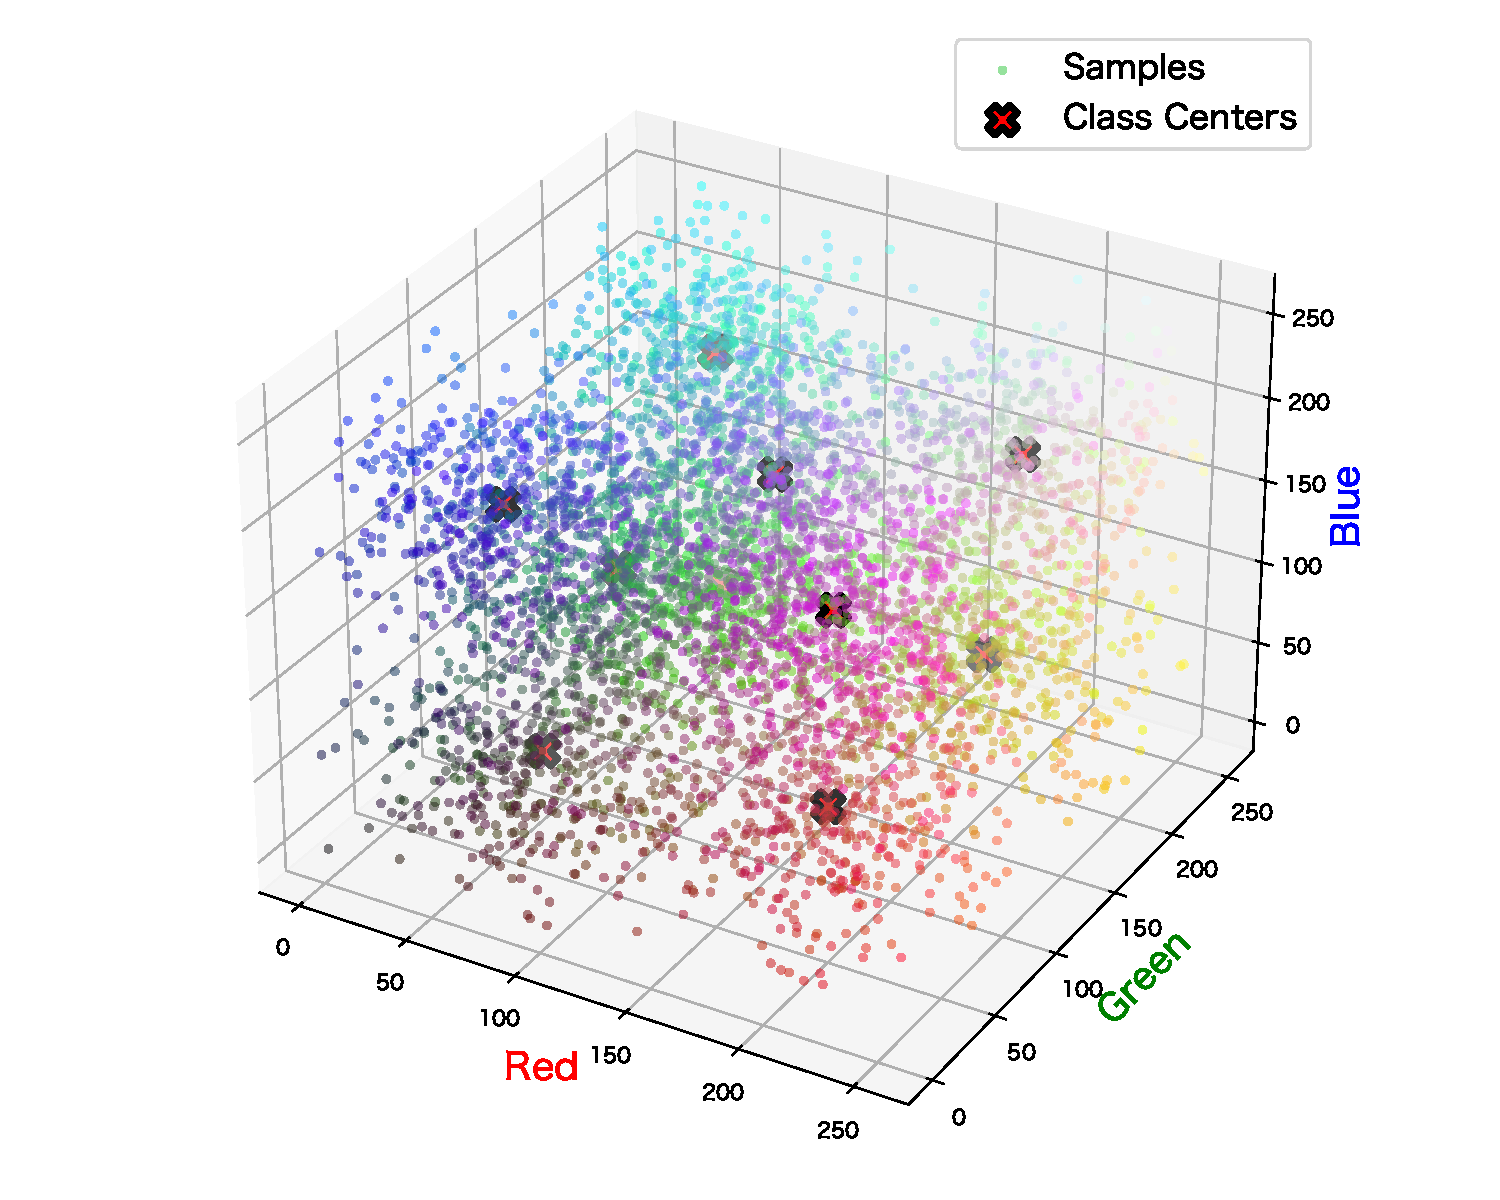
\includegraphics[width=1\columnwidth]{fig/DistributionColors.pdf}
    \caption[RGB色空間における10種類の色クラスの分布を示した3次元散布図]{
        RGB色空間における10種類の色クラスの分布を示した3次元散布図.
        各色クラスはk-means法を用いて均等に分布するよう決定されており,各クラスの中心が赤い「X」マーカーで強調表示されている.
        これにより,色クラス間の平均距離がほぼ均等となり,色概念の識別が均一に行えるような条件が設定されている.
        周囲の点はそれぞれのクラス中心を基準に生成されたサンプルを表し,適度なばらつきを持ちながらも,
        クラス間の明確な分離が保たれている.
    }
    \label{fig:DistributionColors}
\end{figure}

\begin{figure}[H]
    \centering
    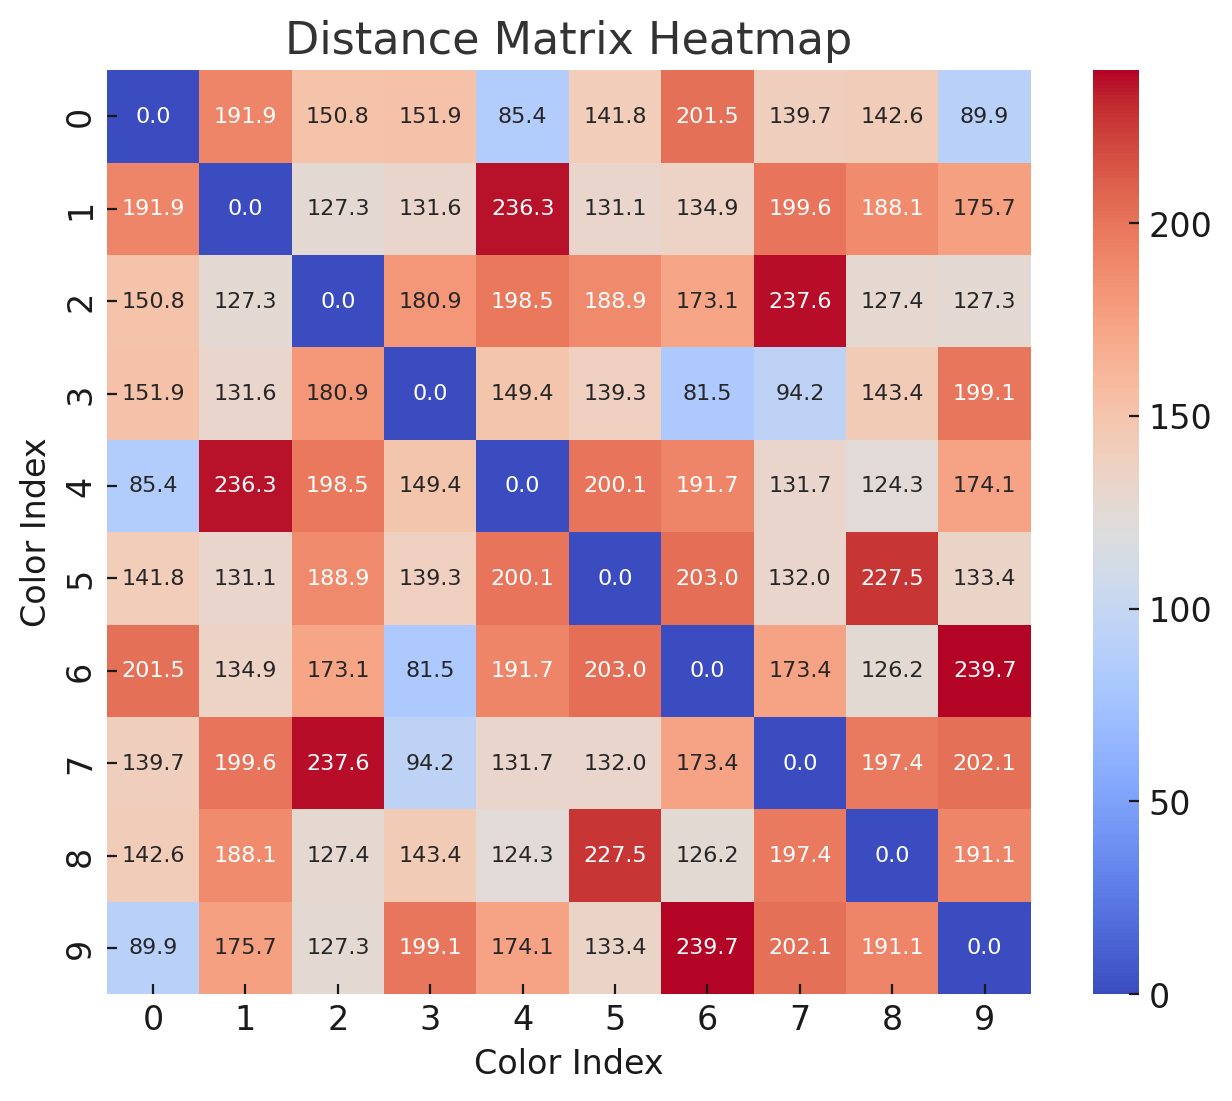
\includegraphics[width=\columnwidth]{tables/Distance_Matrix_Heatmap_color.png}
    \caption[色クラス間の平均距離を示すヒートマップ.]{
        色クラス間の平均距離を示すヒートマップ.
        各セルは,対応する色クラス間の平均距離を示しており,色クラス間の距離が均等に分布していることが確認できる.
    }
    \label{fig:color_class_distance}
\end{figure}

\begin{figure}[H]
    \centering
    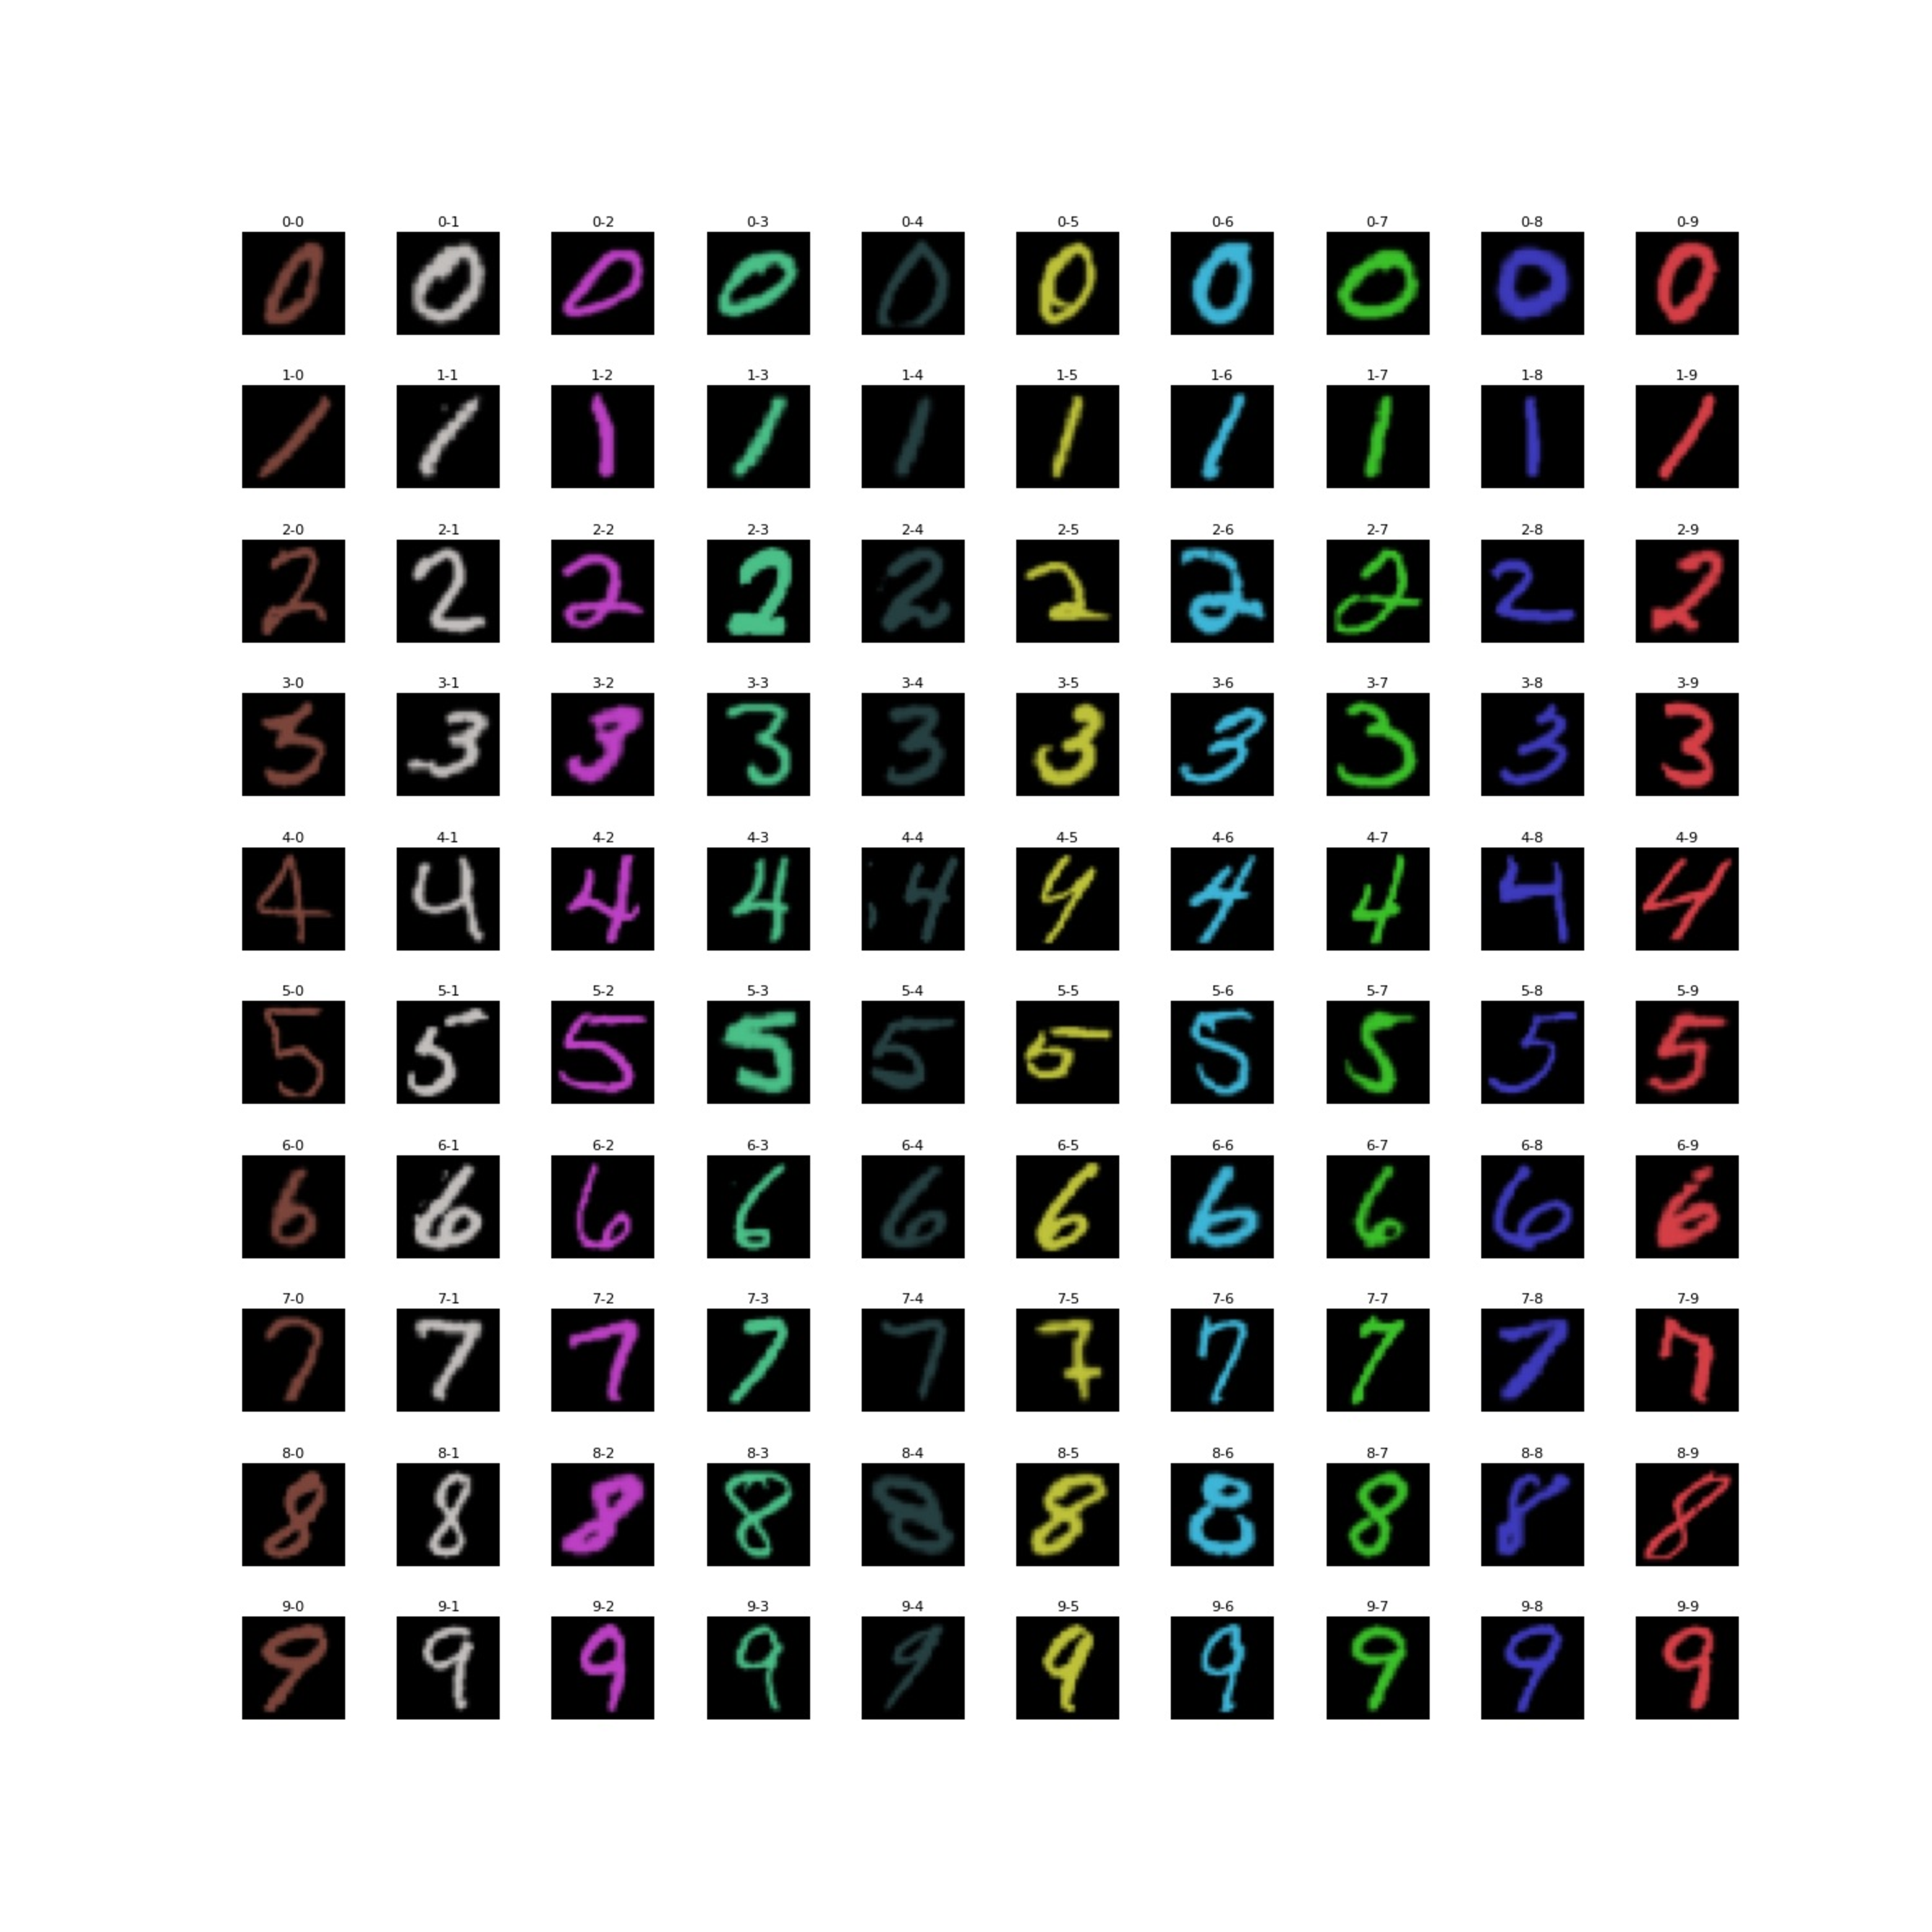
\includegraphics[width=1\columnwidth]{fig/coloredemnist_0.pdf}
    \caption[Colored EMNISTデータセットの画像例.]{
        Colored EMNISTデータセットの画像例.
        各数字クラス(0-9)に対して,10種類の色クラスがランダムに割り当てられている.
        このデータセットは,数字と色の概念を組み合わせた合計100クラスの分類タスクを提供する.
        行が数字クラス,列が色クラスを示しており,各セルは数字クラスと色クラスの組み合わせに対応する画像を示している.
    }
    \label{fig:ColoredEMNIST}
\end{figure}

\newpage

\section{色概念における難易度調整手法}
色概念の難易度は,RGB値のばらつきを示すパラメータ$\sigma^2$によって制御される.
この手法には以下の特徴がある:$\sigma^2$はすべての色クラスで一定とし,3次元空間でバランスの取れた色分布を実現する.
色概念間の識別に関するBayes errorを$\sigma^2$によって制御することが可能である.
$\sigma = 0$の場合,代表RGB値のみが付与される.$\sigma = 10\sqrt{10}$,$\sigma = 100$では,
色クラスの分布がより広がり,色概念の識別がより困難になる.
図\ref{fig:coloredeminsts}に,$\sigma^2 = 0, 10^3, 10^{3.5}, 10^4$の場合の画像例を示す.

\begin{figure}[H]
    \centering
    \begin{subfigure}[b]{0.48\textwidth}
        \centering
        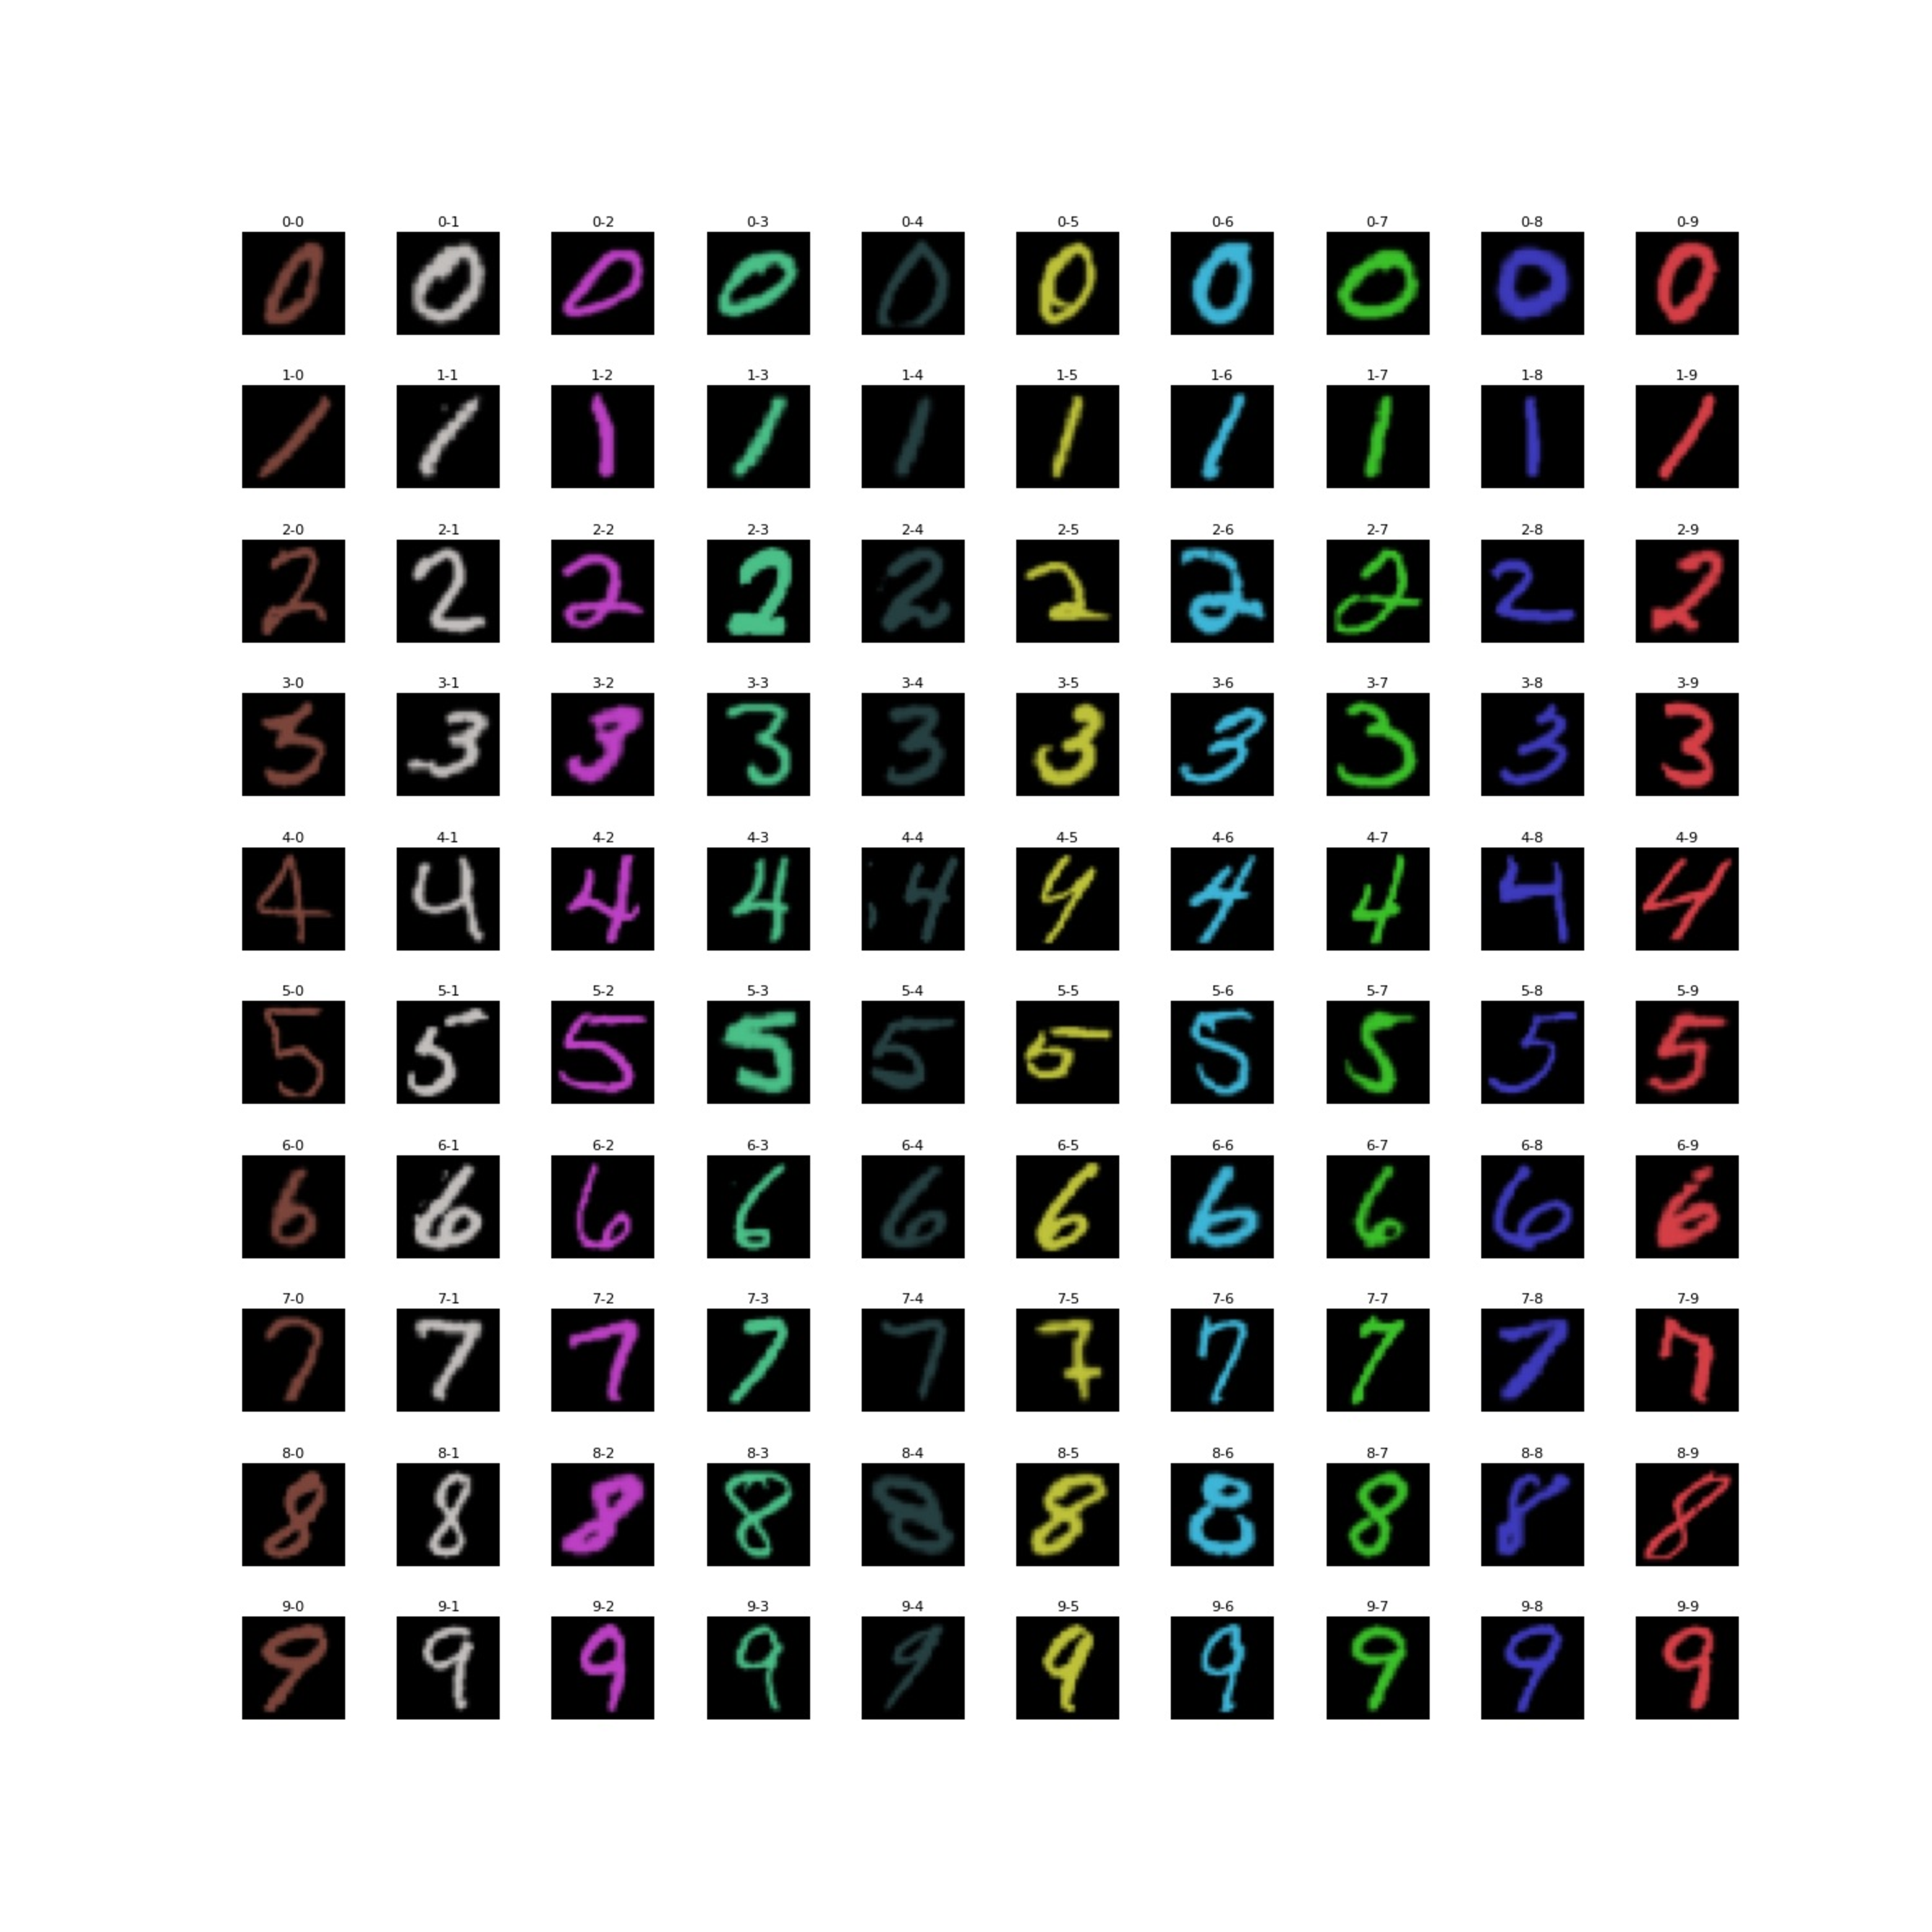
\includegraphics[width=\textwidth]{fig/coloredemnist_0.pdf}
        \caption{$\sigma^2 = 0$}
        \label{fig:coloredeminst_0}
    \end{subfigure}
    \hfill
    \begin{subfigure}[b]{0.48\textwidth}
        \centering
        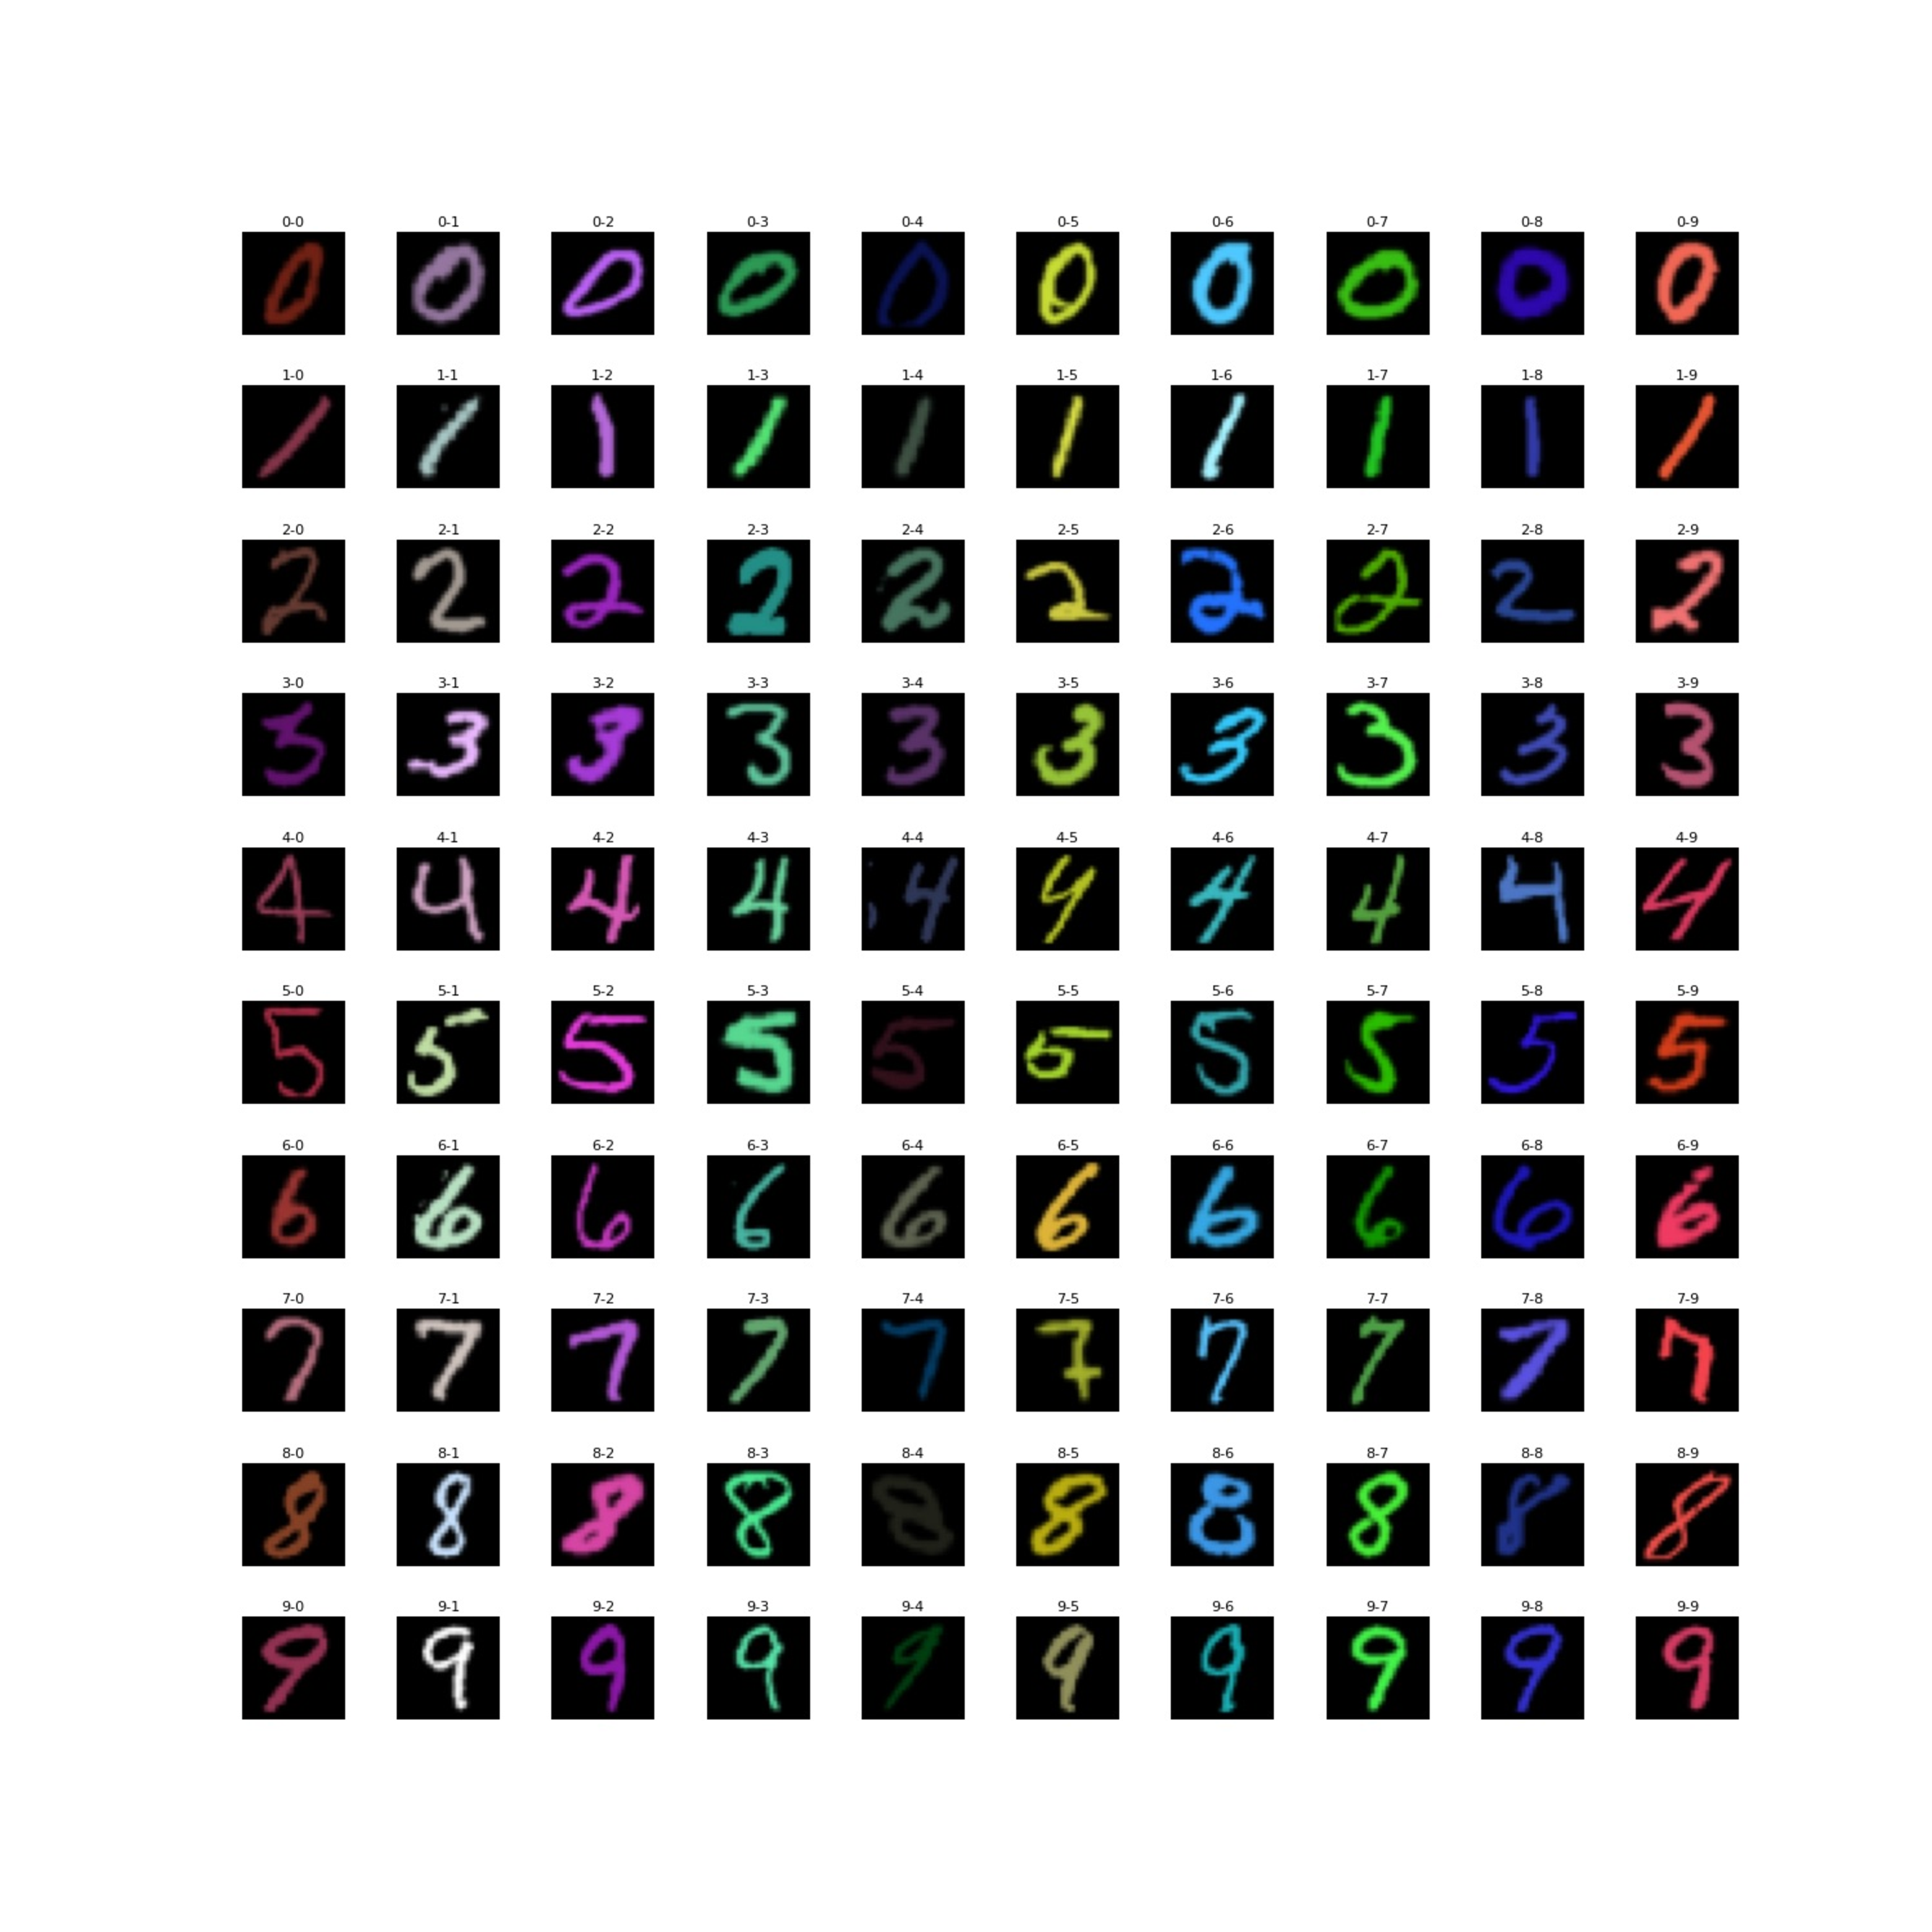
\includegraphics[width=\textwidth]{fig/coloredemnist_1000.pdf}
        \caption{$\sigma^2 = 10^3$}
        \label{fig:coloredeminst_1000}
    \end{subfigure}
    \vspace{0.5cm}
    \begin{subfigure}[b]{0.48\textwidth}
        \centering
        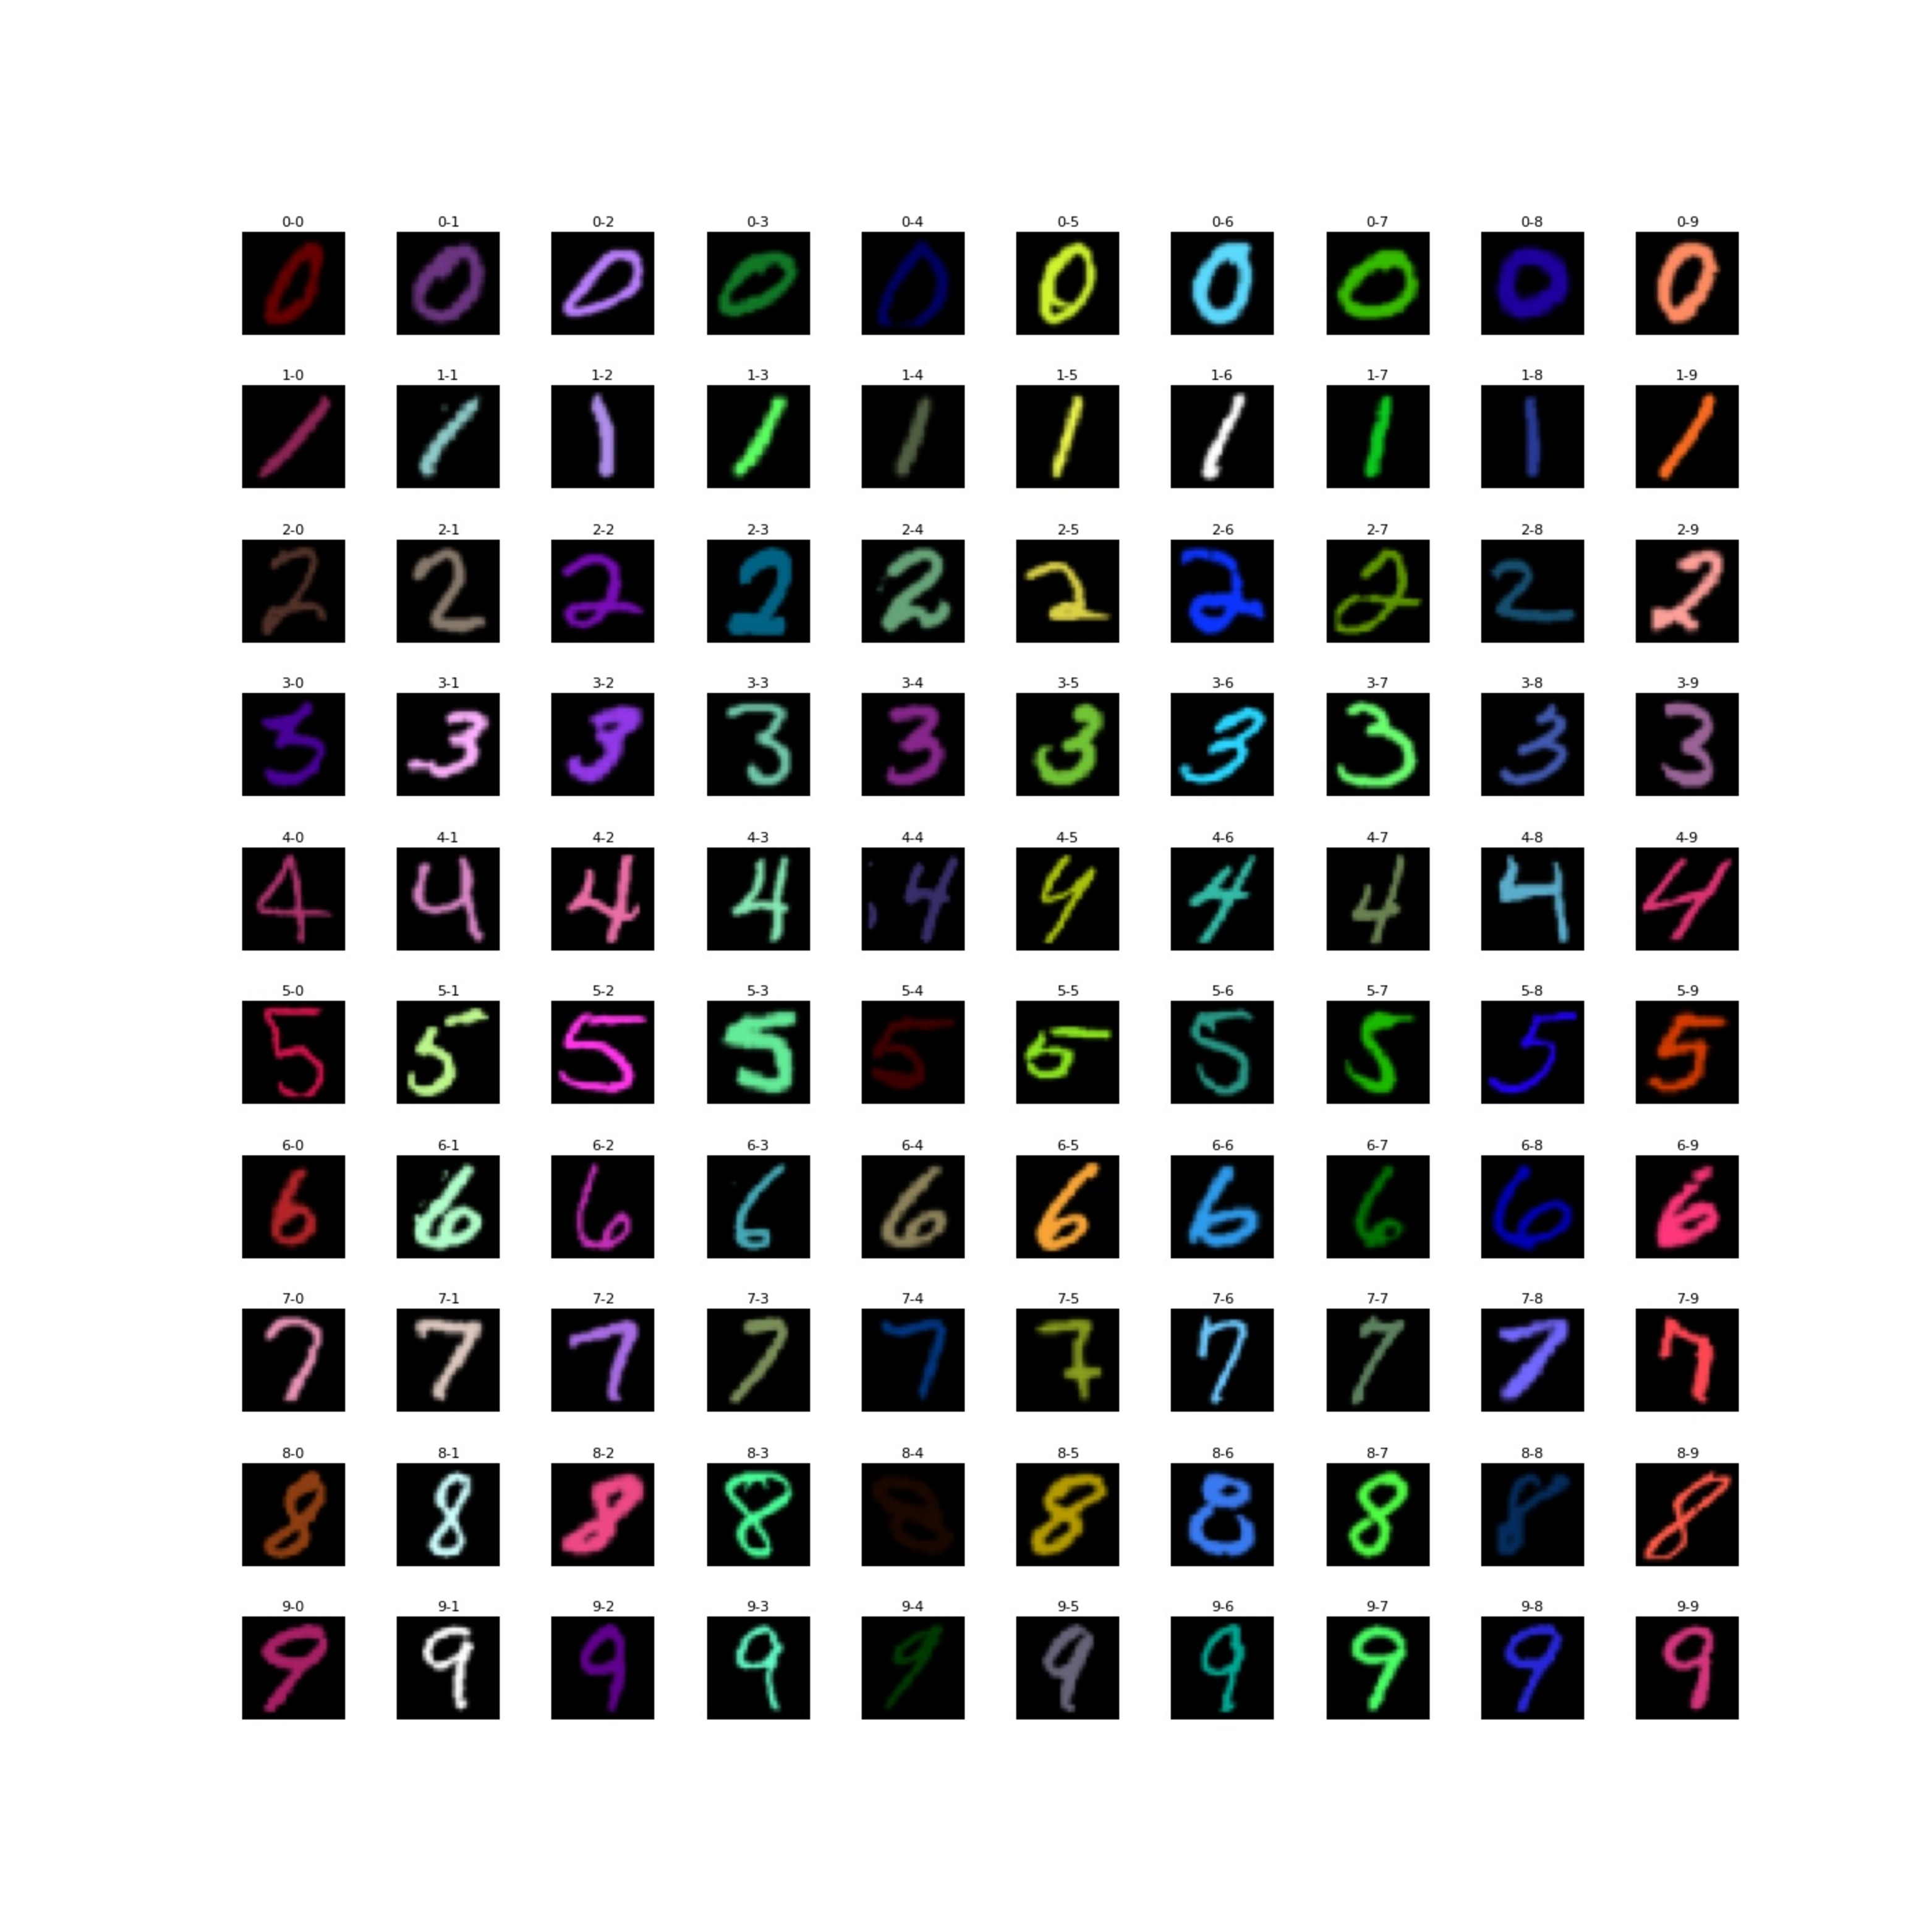
\includegraphics[width=\textwidth]{fig/coloredemnist_3612.pdf}
        \caption{$\sigma^2 = 10^{3.5}$}
        \label{fig:coloredeminst_3612}
    \end{subfigure}
    \hfill
    \begin{subfigure}[b]{0.48\textwidth}
        \centering
        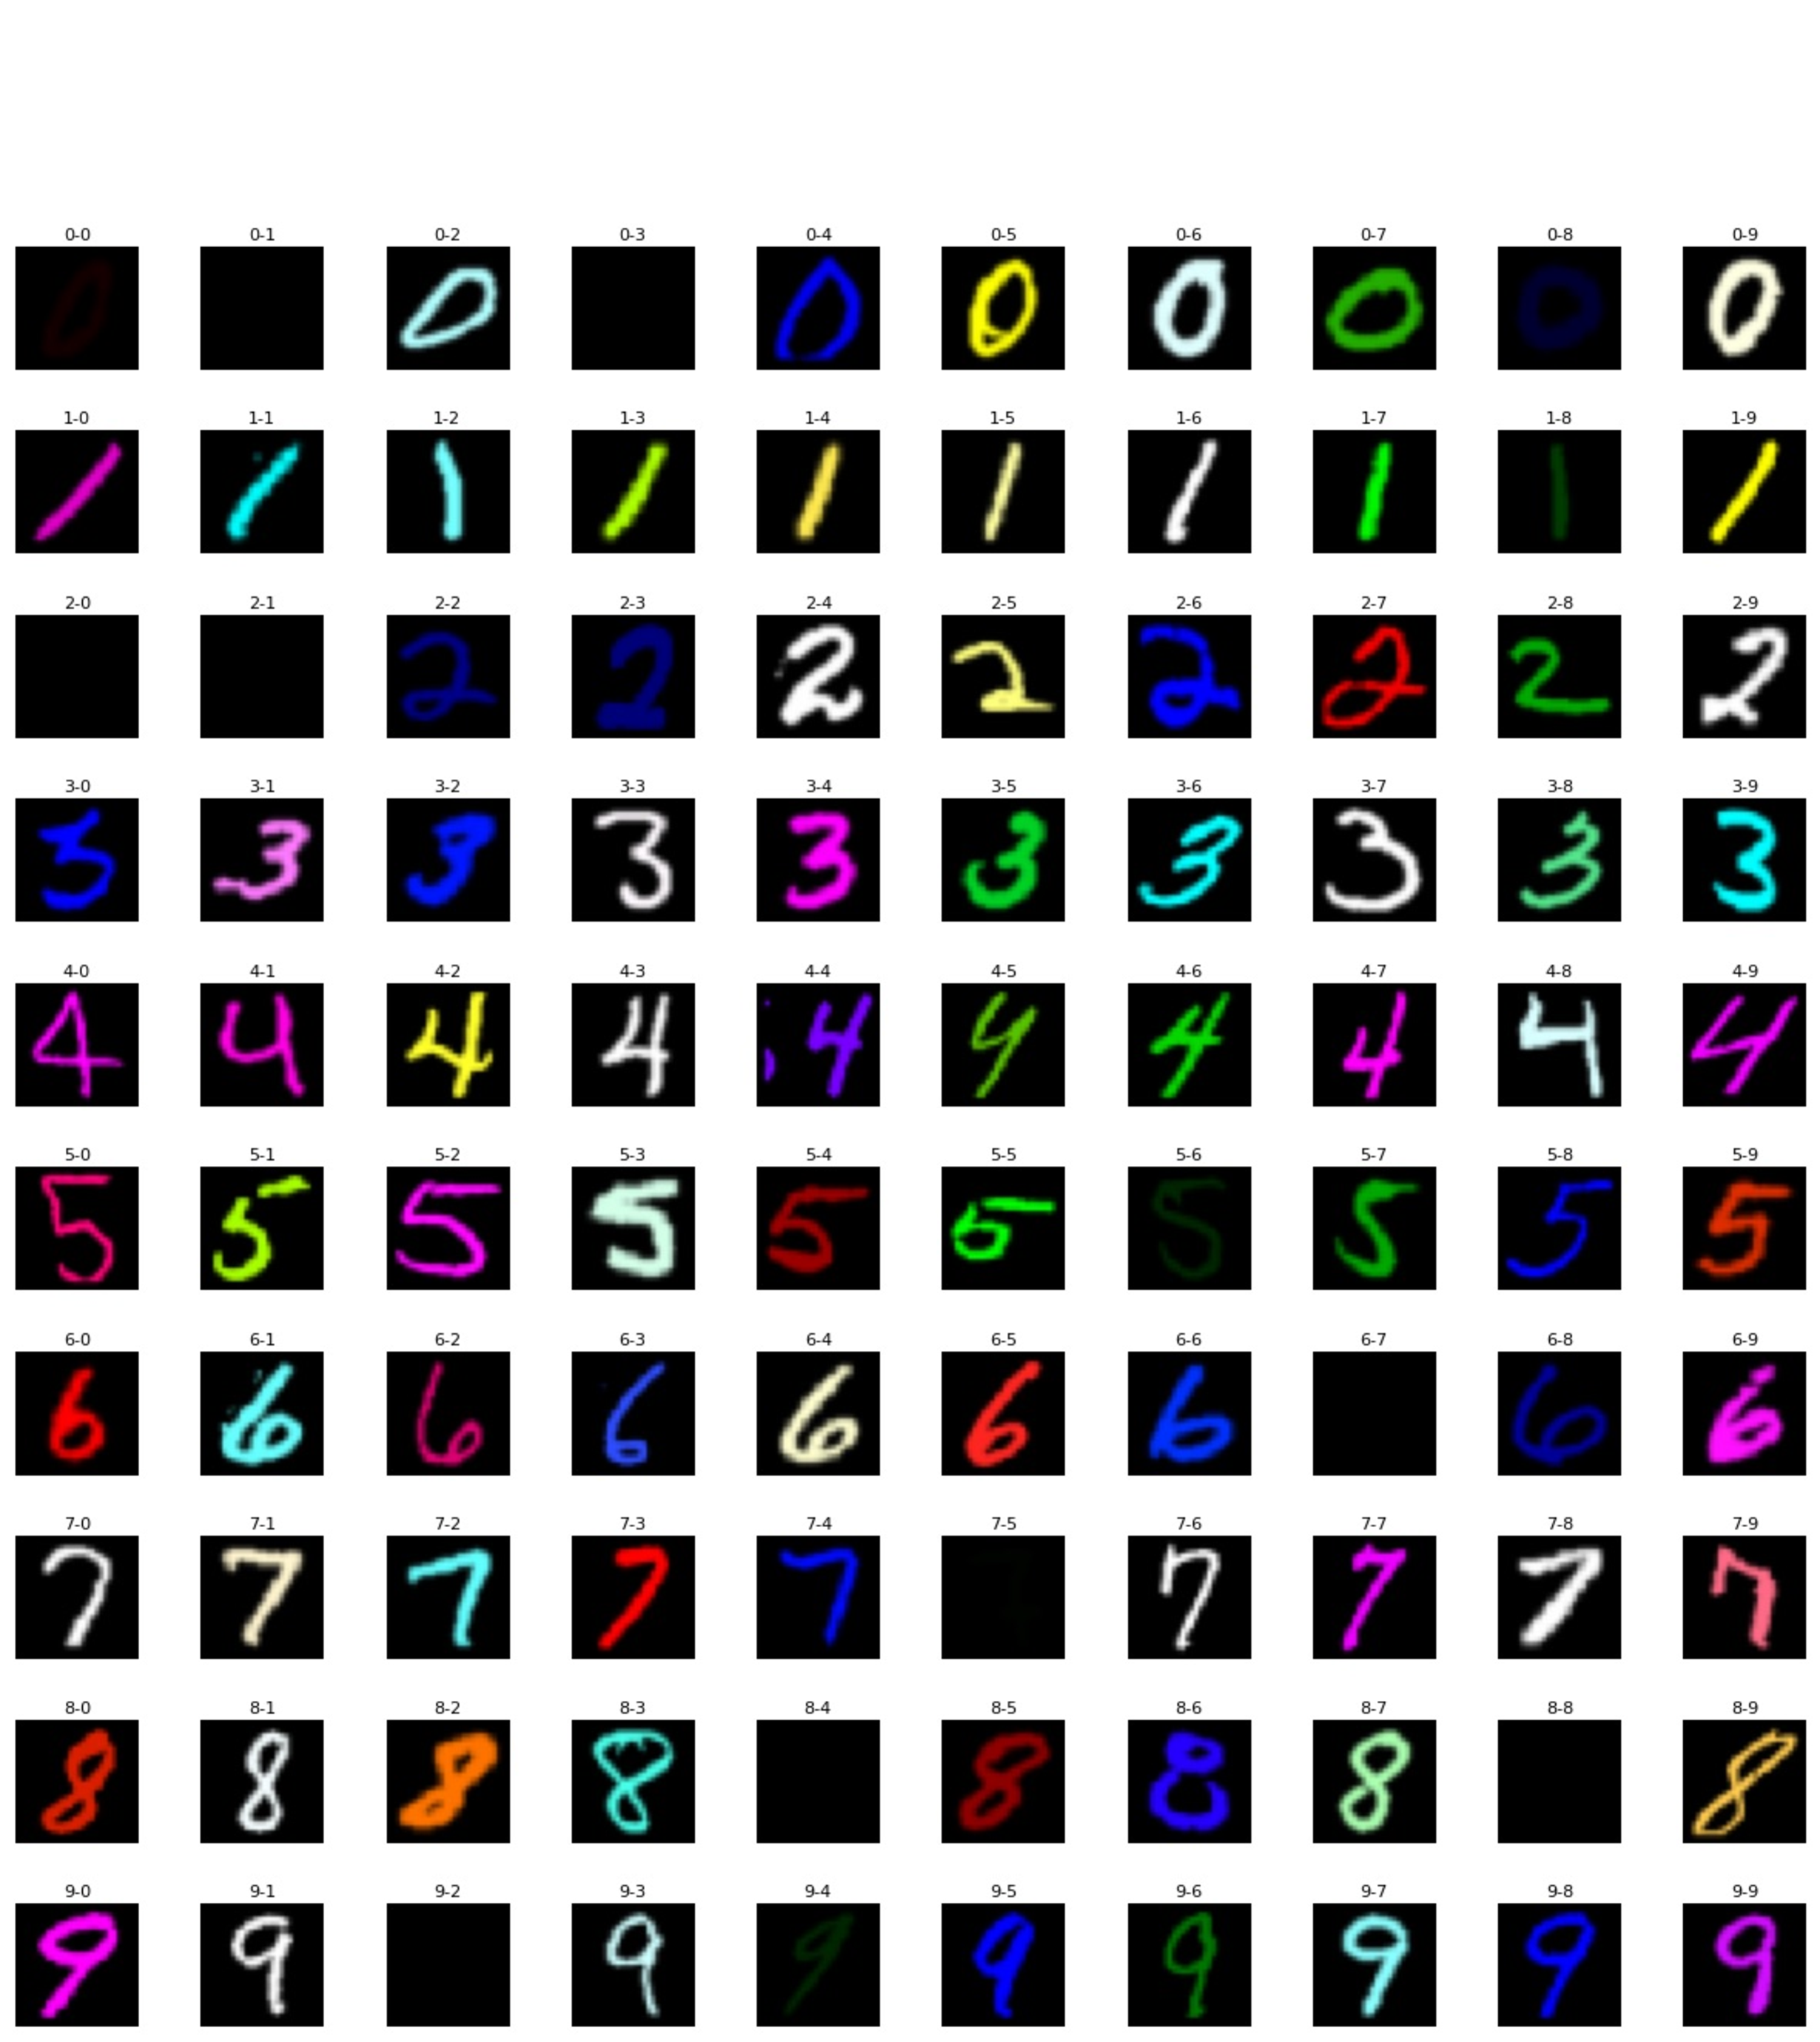
\includegraphics[width=\textwidth]{fig/coloredemnist_10000.pdf}
        \caption{$\sigma^2 = 10^4$}
        \label{fig:coloredeminst_10000}
    \end{subfigure}
    \caption{Colored EMNISTデータセットにおける色概念の難易度調整例.
    100枚の画像において,同じ列が色クラス,行が数字クラスを示している.
    各図は異なるパラメータ$\sigma^2$で生成されたサンプルを示している.$\sigma^2$が増加するにつれて,色概念のばらつきが大きくなる.
    }
    \label{fig:coloredeminsts}
\end{figure}

\section{ラベルノイズの付与}
ラベルノイズは,データセットのラベルに誤りが含まれることを指す.
データセットの品質を低下させる要因の一つであり,機械学習モデルの性能を低下させるほか,二重降下現象を観察するうえで重要な要素である.
本研究では,ラベルノイズを付与することで,モデルのロバスト性や学習効率に関する知見を得ることも目的としている.
ラベルノイズは,各クラスのラベルを一定の確率で別のクラスに置き換えることで実珸される.
ラベルノイズを付与する場合,数字と色のラベルに対してどちらも異なるノイズ率を設定する.


\chapter{実験}
\label{chap:experiment}

本章では,第\ref{chap:experiment_settings}章で提案したデータセットを用いた,実験方法を述べる.
本研究の目的は,色と数字の概念がどのように獲得されるかを学習過程から分析することである.この目的を達成するために,100クラス分類タスクを設定し,訓練データとテストデータにおける詳細なエラー率を観察した.

訓練データに対するエラー率の観察では,以下の条件を設定した(表\ref{tab:train_error}).色と数字の両方を含む概念,色のみの概念,数字のみの概念に対して,それぞれラベルノイズがある場合とない場合の分類エラー率を記録した.

\begin{table}[h]
\centering
\caption{訓練データに対するエラー率の観察条件}
\begin{tabular}{lll}
\toprule
\textbf{概念} & \textbf{ラベルノイズの有無} & \textbf{分類タスク} \\
\midrule
色+数字 & 有・無 & 100クラス分類 \\
色のみ   & 有・無 & 色分類タスク \\
数字のみ & 有・無 & 数字分類タスク \\
\bottomrule
\end{tabular}
\label{tab:train_error}
\end{table}

テストデータに対するエラー率の観察では,ラベルノイズがない条件で,色と数字の両方を含む概念,色のみの概念,数字のみの概念に対するエラー率を記録した(表\ref{tab:test_error}).

\begin{table}[h]
\centering
\caption{テストデータに対するエラー率の観察条件}
\begin{tabular}{lll}
\toprule
\textbf{概念} & \textbf{ラベルノイズの有無} & \textbf{分類タスク} \\
\midrule
色+数字 & 無 & 100クラス分類 \\
色のみ   & 無 & 色分類タスク \\
数字のみ & 無 & 数字分類タスク \\
\bottomrule
\end{tabular}
\label{tab:test_error}
\end{table}

これらの設定を通じて,色と数字の概念が獲得される過程と,ラベルノイズの有無が分類性能に与える影響について詳細に分析することを目指した.

\newpage

\section{実験設定}
\label{sec:experiment_settings}
実験設定において,提案したデータセットに基づき,小程度から大程度までのCNNモデルを用いて学習を行う.
今回の実験においては,5層のCNN,8層のCNN,そして,16層のCNNを使って,学習過程を観察した.
今回は,訓練データとテストデータに関して,以下の学習曲線を観察し,詳細な学習過程の分析を行う.その観察した学習曲線は,以下の通りである.


また,5層と8層のモデルにおいて,Model Widthを変化させ,モデルキャパシティを変更したときの学習過程を観察した.

以下に詳細な実験設定を示す.

\begin{table}[ht]
    \centering
    \caption{モデル設定}
    \begin{tabular}{ll}
        \midrule
        Model Layers & 5, 8, 16 \\
        Model Width & 1, 2, 4, 8 \\
        \bottomrule
    \end{tabular}
    \label{tab:model_settings}
\end{table}

また,これらの学習のパラメータを以下に示す.

\begin{table}[ht]
    \centering
    \caption{学習設定}
    \begin{tabular}{ll}
        \toprule
        \textbf{Parameter} & \textbf{Values} \\
        \midrule
        Epochs & 1000 \\
        Batch Size & 256 \\
        Learning Rate & 0.01 \\
        Optimizer & SGD \\
        Momentum & 0.0 \\
        Loss Function & Cross Entropy \\
        \bottomrule
    \end{tabular}
    \label{tab:training_settings}
\end{table}

これらのCNNモデルの構造を表\ref{tab:cnn5layer},表\ref{tab:cnn8layer},表\ref{tab:cnn16layer}に示す.
Width Multiplierは,モデルの幅を調整するためのパラメータである.

\begin{table}[h]
    \centering
    \caption{5層のCNNのアーキテクチャ}
    \label{tab:cnn5layer}
    \begin{tabular}{lll}
    \toprule
    \textbf{Layer} & \textbf{Output Shape} & \textbf{Details} \\
    \midrule
    Input & $3 \times 32 \times 32$ & RGB image \\
    Conv1 & $16 \cdot \text{width multiplier} \times 32 \times 32$ & $3 \times 3$ kernel, stride 1, padding 1 \\
    ReLU1 & Same as above & Activation \\
    MaxPool1 & $16 \cdot \text{width multiplier} \times 16 \times 16$ & $2 \times 2$ kernel, stride 2 \\
    Conv2 & $32 \cdot \text{width multiplier} \times 16 \times 16$ & $3 \times 3$ kernel, stride 1, padding 1 \\
    ReLU2 & Same as above & Activation \\
    MaxPool2 & $32 \cdot \text{width multiplier} \times 8 \times 8$ & $2 \times 2$ kernel, stride 2 \\
    Conv3 & $64 \cdot \text{width multiplier} \times 8 \times 8$ & $3 \times 3$ kernel, stride 1, padding 1 \\
    ReLU3 & Same as above & Activation \\
    Conv4 & $128 \cdot \text{width multiplier} \times 8 \times 8$ & $3 \times 3$ kernel, stride 1, padding 1 \\
    ReLU4 & Same as above & Activation \\
    MaxPool4 & $128 \cdot \text{width multiplier} \times 4 \times 4$ & $2 \times 2$ kernel, stride 2 \\
    Conv5 & $256 \cdot \text{width multiplier} \times 4 \times 4$ & $3 \times 3$ kernel, stride 1, padding 1 \\
    ReLU5 & Same as above & Activation \\
    Fully Connected & $256 \cdot (\text{img size}/8)^2 \times 100$ & Output: 100 classes \\
    \bottomrule
    \end{tabular}
\end{table}

\begin{table}[h]
    \centering
    \caption{8層のCNNのアーキテクチャ}
    \label{tab:cnn8layer}
    \begin{tabular}{lll}
    \toprule
    \textbf{Layer} & \textbf{Output Shape} & \textbf{Details} \\
    \midrule
    Same as CNN5Layer up to Conv5 & & \\
    Conv6 & $512 \cdot \text{width multiplier} \times 4 \times 4$ & $3 \times 3$ kernel, stride 1, padding 1 \\
    ReLU6 & Same as above & Activation \\
    MaxPool6 & $512 \cdot \text{width multiplier} \times 2 \times 2$ & $2 \times 2$ kernel, stride 2 \\
    Conv7 & $512 \cdot \text{width multiplier} \times 2 \times 2$ & $3 \times 3$ kernel, stride 1, padding 1 \\
    ReLU7 & Same as above & Activation \\
    Conv8 & $512 \cdot \text{width multiplier} \times 2 \times 2$ & $3 \times 3$ kernel, stride 1, padding 1 \\
    ReLU8 & Same as above & Activation \\
    Fully Connected & $512 \cdot (\text{img size}/16)^2 \times 100$ & Output: 100 classes \\
    \bottomrule
    \end{tabular}
\end{table}

\begin{table}[h]
    \centering
    \caption{16層CNNのアーキテクチャ}
    \label{tab:cnn16layer}
    \begin{tabular}{lll}
    \toprule
    \textbf{Layer} & \textbf{Output Shape} & \textbf{Details} \\
    \midrule
    Input & $3 \times 32 \times 32$ & RGB image \\
    Conv1 & $64 \cdot \text{width multiplier} \times 32 \times 32$ & $3 \times 3$ kernel, stride 1, padding 1 \\
    BatchNorm1 & Same as above & Normalization \\
    ReLU1 & Same as above & Activation \\
    Conv2 & $64 \cdot \text{width multiplier} \times 32 \times 32$ & $3 \times 3$ kernel, stride 1, padding 1 \\
    BatchNorm2 & Same as above & Normalization \\
    ReLU2 & Same as above & Activation \\
    MaxPool2 & $64 \cdot \text{width multiplier} \times 16 \times 16$ & $2 \times 2$ kernel, stride 2 \\
    Conv3 & $128 \cdot \text{width multiplier} \times 16 \times 16$ & $3 \times 3$ kernel, stride 1, padding 1 \\
    BatchNorm3 & Same as above & Normalization \\
    ReLU3 & Same as above & Activation \\
    Conv4 & $128 \cdot \text{width multiplier} \times 16 \times 16$ & $3 \times 3$ kernel, stride 1, padding 1 \\
    BatchNorm4 & Same as above & Normalization \\
    ReLU4 & Same as above & Activation \\
    MaxPool4 & $128 \cdot \text{width multiplier} \times 8 \times 8$ & $2 \times 2$ kernel, stride 2 \\
    Conv5-7 & $256 \cdot \text{width multiplier} \times 8 \times 8$ & $3 \times (3 \times 3$ kernel, stride 1, padding 1) \\
    BatchNorm5-7 & Same as above & $3 \times$ Normalization \\
    ReLU5-7 & Same as above & $3 \times$ Activation \\
    MaxPool7 & $256 \cdot \text{width multiplier} \times 4 \times 4$ & $2 \times 2$ kernel, stride 2 \\
    Conv8-10 & $512 \cdot \text{width multiplier} \times 4 \times 4$ & $3 \times (3 \times 3$ kernel, stride 1, padding 1) \\
    BatchNorm8-10 & Same as above & $3 \times$ Normalization \\
    ReLU8-10 & Same as above & $3 \times$ Activation \\
    MaxPool10 & $512 \cdot \text{width multiplier} \times 2 \times 2$ & $2 \times 2$ kernel, stride 2 \\
    Conv11-13 & $512 \cdot \text{width multiplier} \times 2 \times 2$ & $3 \times (3 \times 3$ kernel, stride 1, padding 1) \\
    BatchNorm11-13 & Same as above & $3 \times$ Normalization \\
    ReLU11-13 & Same as above & $3 \times$ Activation \\
    MaxPool13 & $512 \cdot \text{width multiplier} \times 1 \times 1$ & $2 \times 2$ kernel, stride 2 \\
    Conv14-16 & $512 \cdot \text{width multiplier} \times 1 \times 1$ & $3 \times (3 \times 3$ kernel, stride 1, padding 1) \\
    BatchNorm14-16 & Same as above & $3 \times$ Normalization \\
    ReLU14-16 & Same as above & $3 \times$ Activation \\
    Dropout & Same as above & Rate: 0.5 \\
    Fully Connected & $512 \cdot (\text{img size}/32)^2 \times 100$ & Output: 100 classes \\
    \bottomrule
    \end{tabular}
\end{table}


\chapter{結果}
\label{chap:results}

\subsection{ラベルノイズ付与による変化}
$\sigma$別に,それぞれのラベルノイズにおける詳細なエラー率を図\ref{fig:errors_by_label_noise_variance_0},図\ref{fig:coloredeminst_1000},図\ref{fig:errors_by_label_noise_variance_3612}
図\ref{fig:coloredeminst_10000}にそれぞれ示す.
特に$\gamma$が付与されている結果において,3つのフェーズに分けることができる.
\begin{itemize}
    \item Phase1 : テストエラー率と訓練エラー率がともに低下する.
    \item Phase2 : 訓練エラー率は引き続き低下するが,テストエラー率は上昇に転じる.
    \item Phase3 : 訓練エラー率はさらに低下するが,テストエラー率の上昇は緩やかになる.
\end{itemize}
色と数字の学習に関して,色よりも数字のほうが訓練・テストエラー率が高いことから,数字よりも色の難易度が低く,学習しやすいことが確認できる.
5層のCNNに関して,Phase1では,中段の結果を見ると興味深いことに,Colorの誤り率が50\% あたりで低下が停止し,Digitの精度向上を待っているような学習曲線を確認できる.
そして,どちらも50\% の訓練データに対する,誤り率が到達した後に,さらに低下を同時に始める.また,Phase2,3 においては,訓練データに対する誤り率をラベルノイズあり・
なしで分けた結果を確認すると,ラベルノイズなしの誤り率で二重降下現象のような挙動を確認できる.ラベルノイズありに対する誤り率とテストデータに対する誤り率はPhase2,3において,
低下し続けている.これらの低下に関しては,後述する8層のCNNでも同じような挙動を示している.
また,このラベルノイズに対する挙動は,Nakkiranの二重降下現象を確認した設定でも確認した.5層のCNNモデルにおける$\sigma$別の結果を図\ref{fig:errors_by_label_noise_variance_0},図\ref{fig:errors_by_label_noise_variance_1000},
図\ref{fig:errors_by_label_noise_variance_3612}に,Nakkiranの設定における結果を図\ref{fig:errors_by_label_noise_variance_10000}に示す.
\begin{figure}[H]
    \centering
    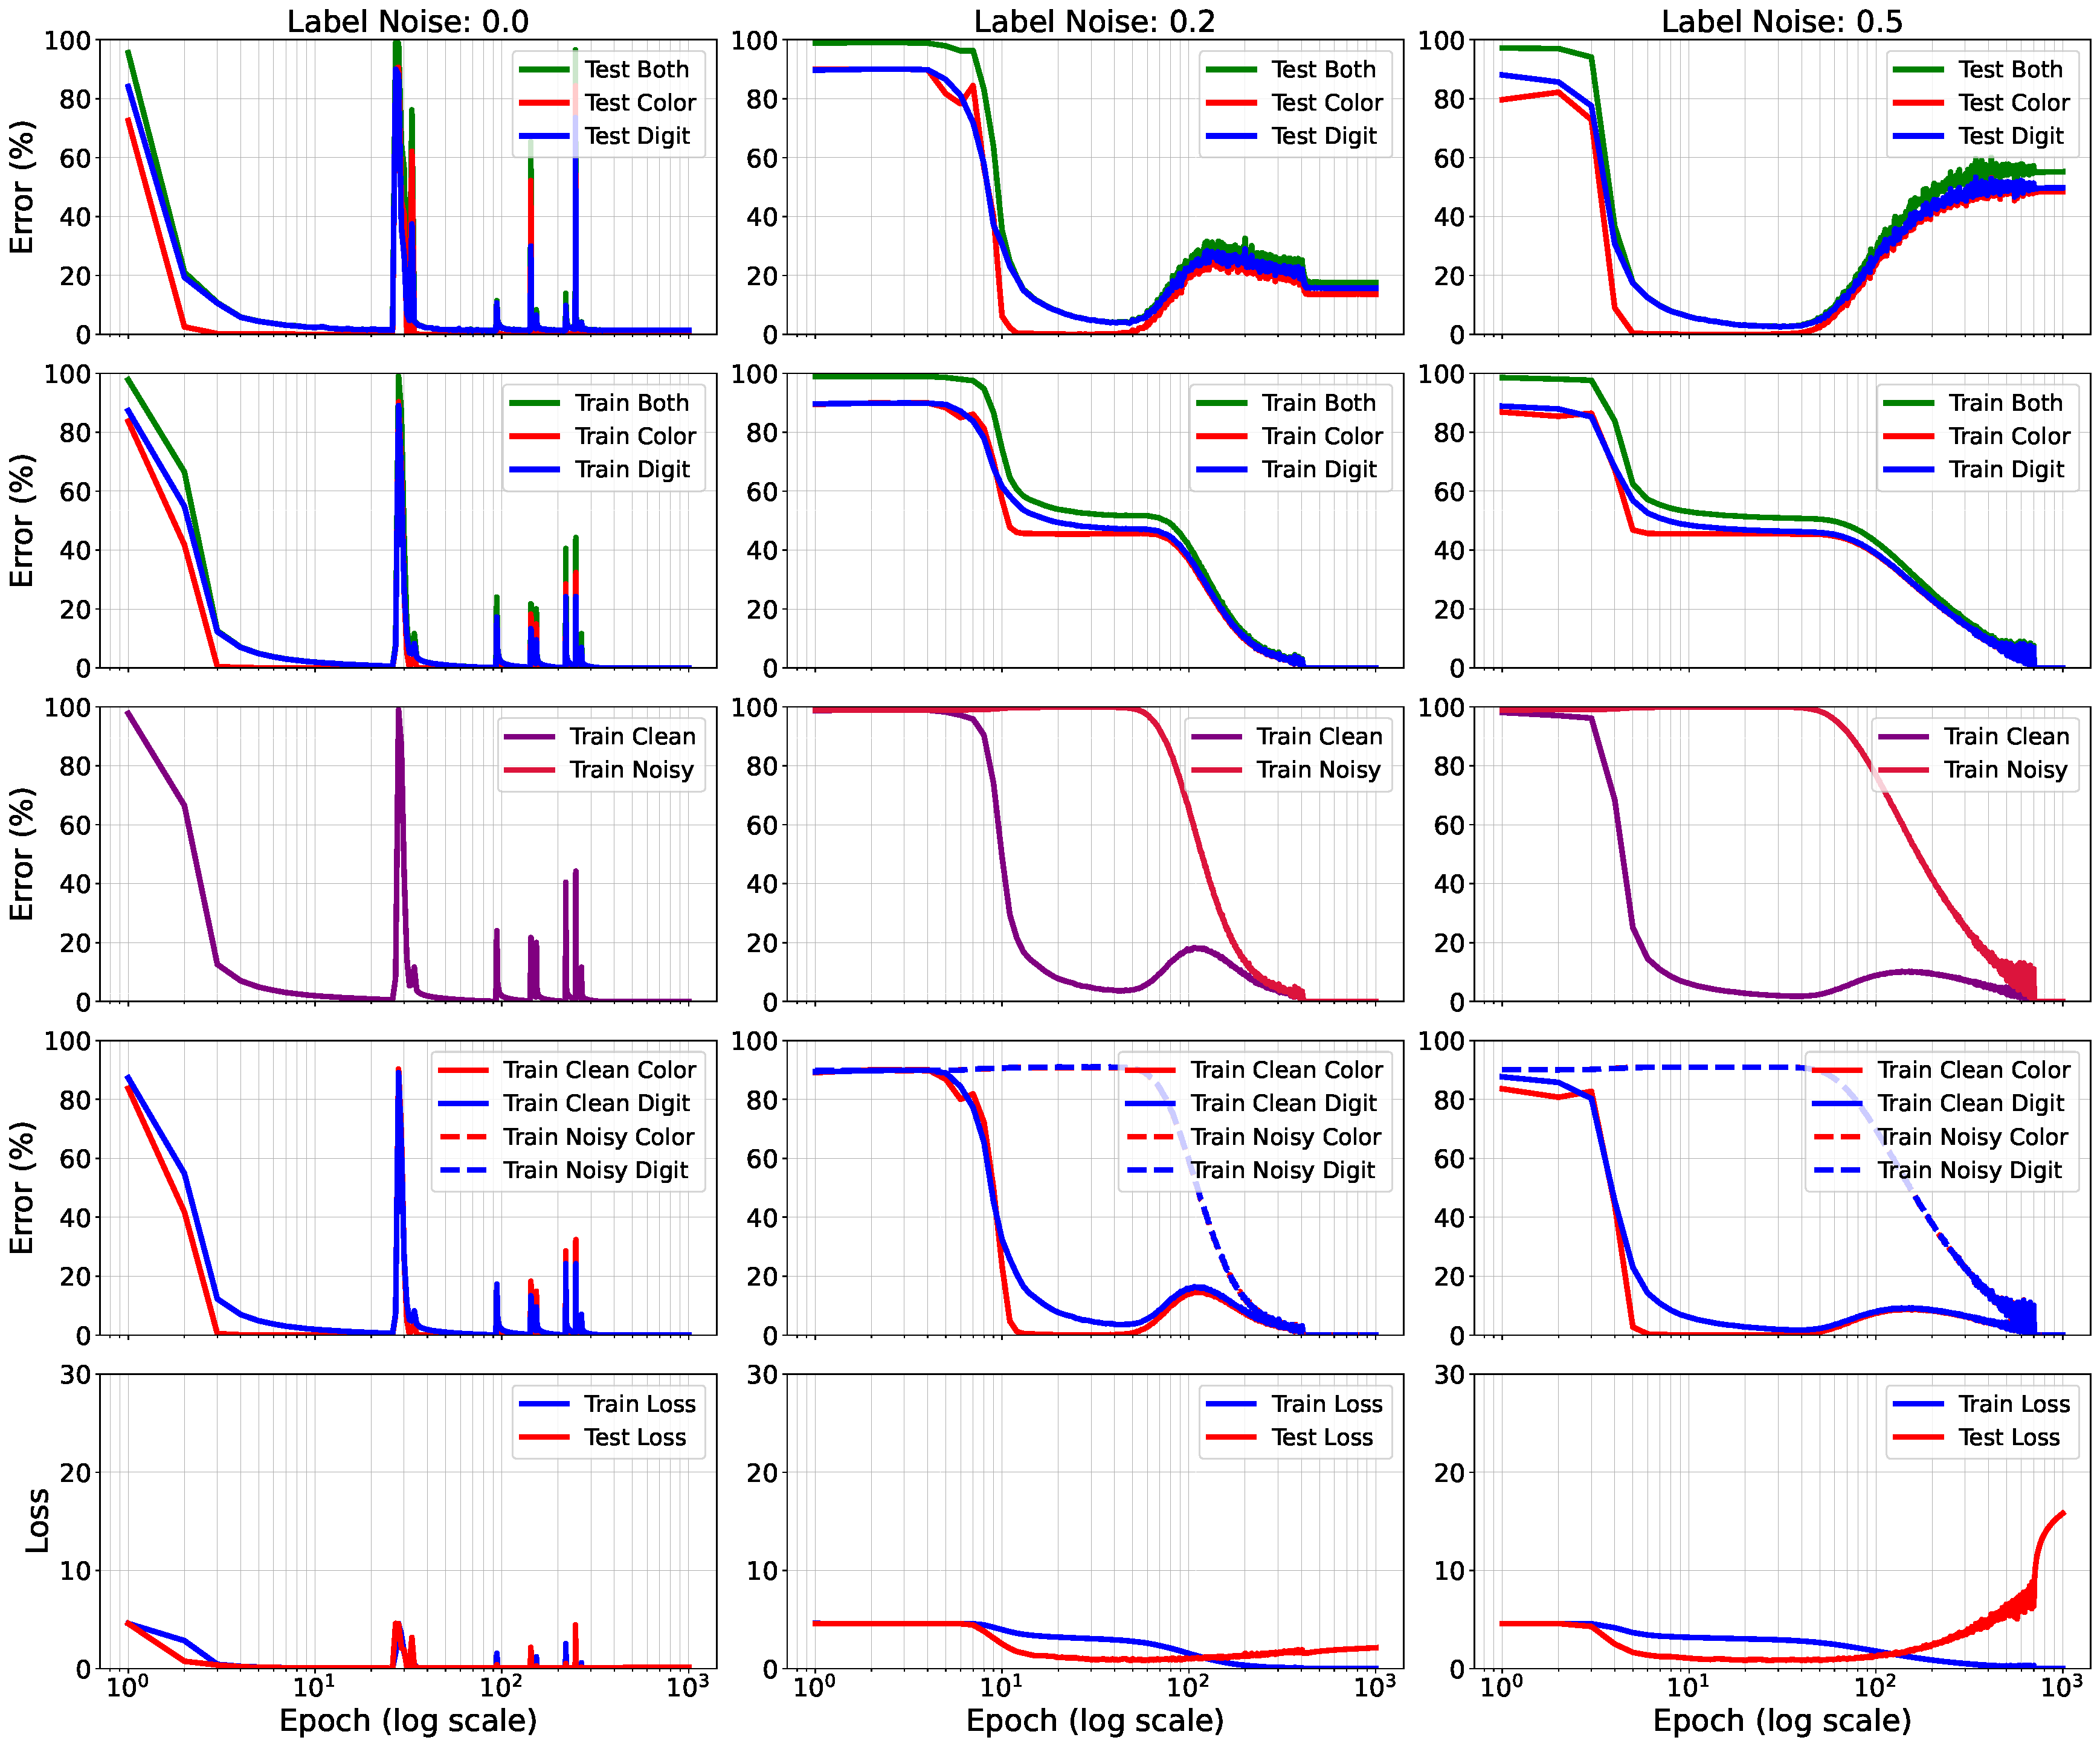
\includegraphics[width=\linewidth]{fig/erroe_metrics_by_variances/error_metrics_by_label_noise_variance_0.pdf}
    \caption{$\sigma^2 = 0$のときのそれぞれのラベルノイズにおける結果}
    \label{fig:errors_by_label_noise_variance_0}
\end{figure}

\begin{figure}[H]
    \centering
    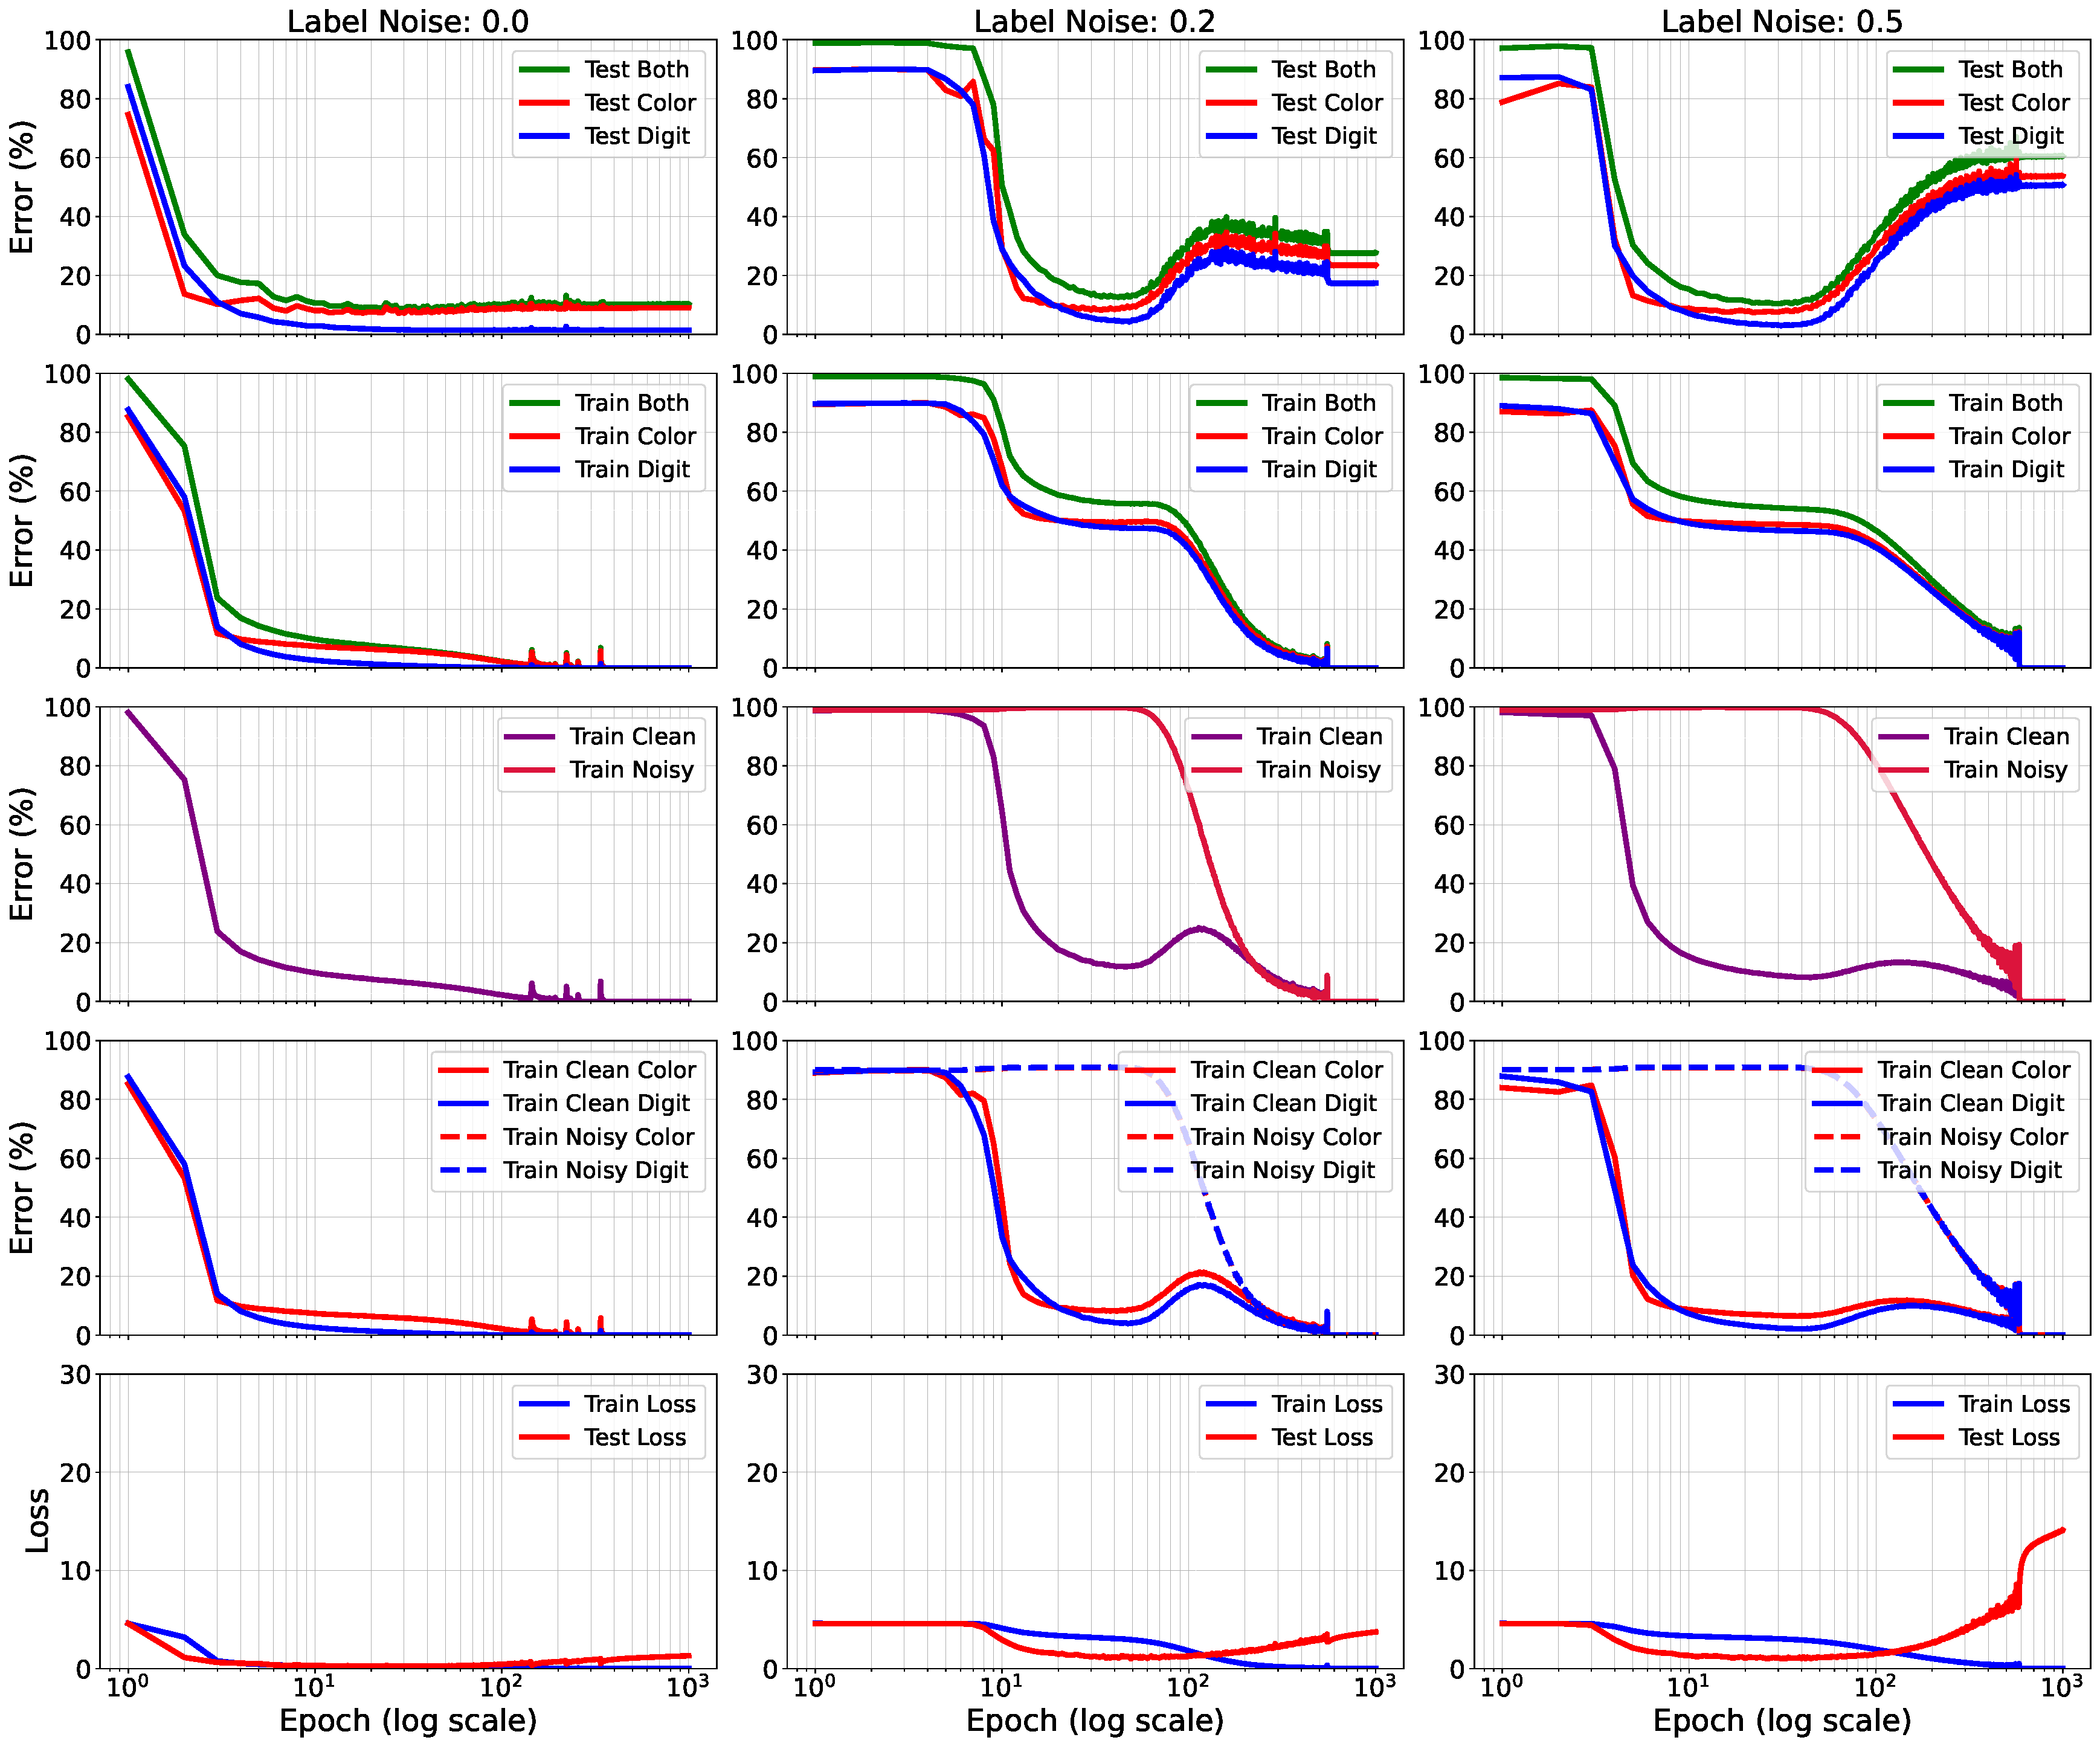
\includegraphics[width=\linewidth]{fig/erroe_metrics_by_variances/error_metrics_by_label_noise_variance_1000.pdf}
    \caption{$\sigma^2 = 10^2$のときのそれぞれのラベルノイズにおける結果}
    \label{fig:errors_by_label_noise_variance_1000}
\end{figure}

\begin{figure}[H]
    \centering
    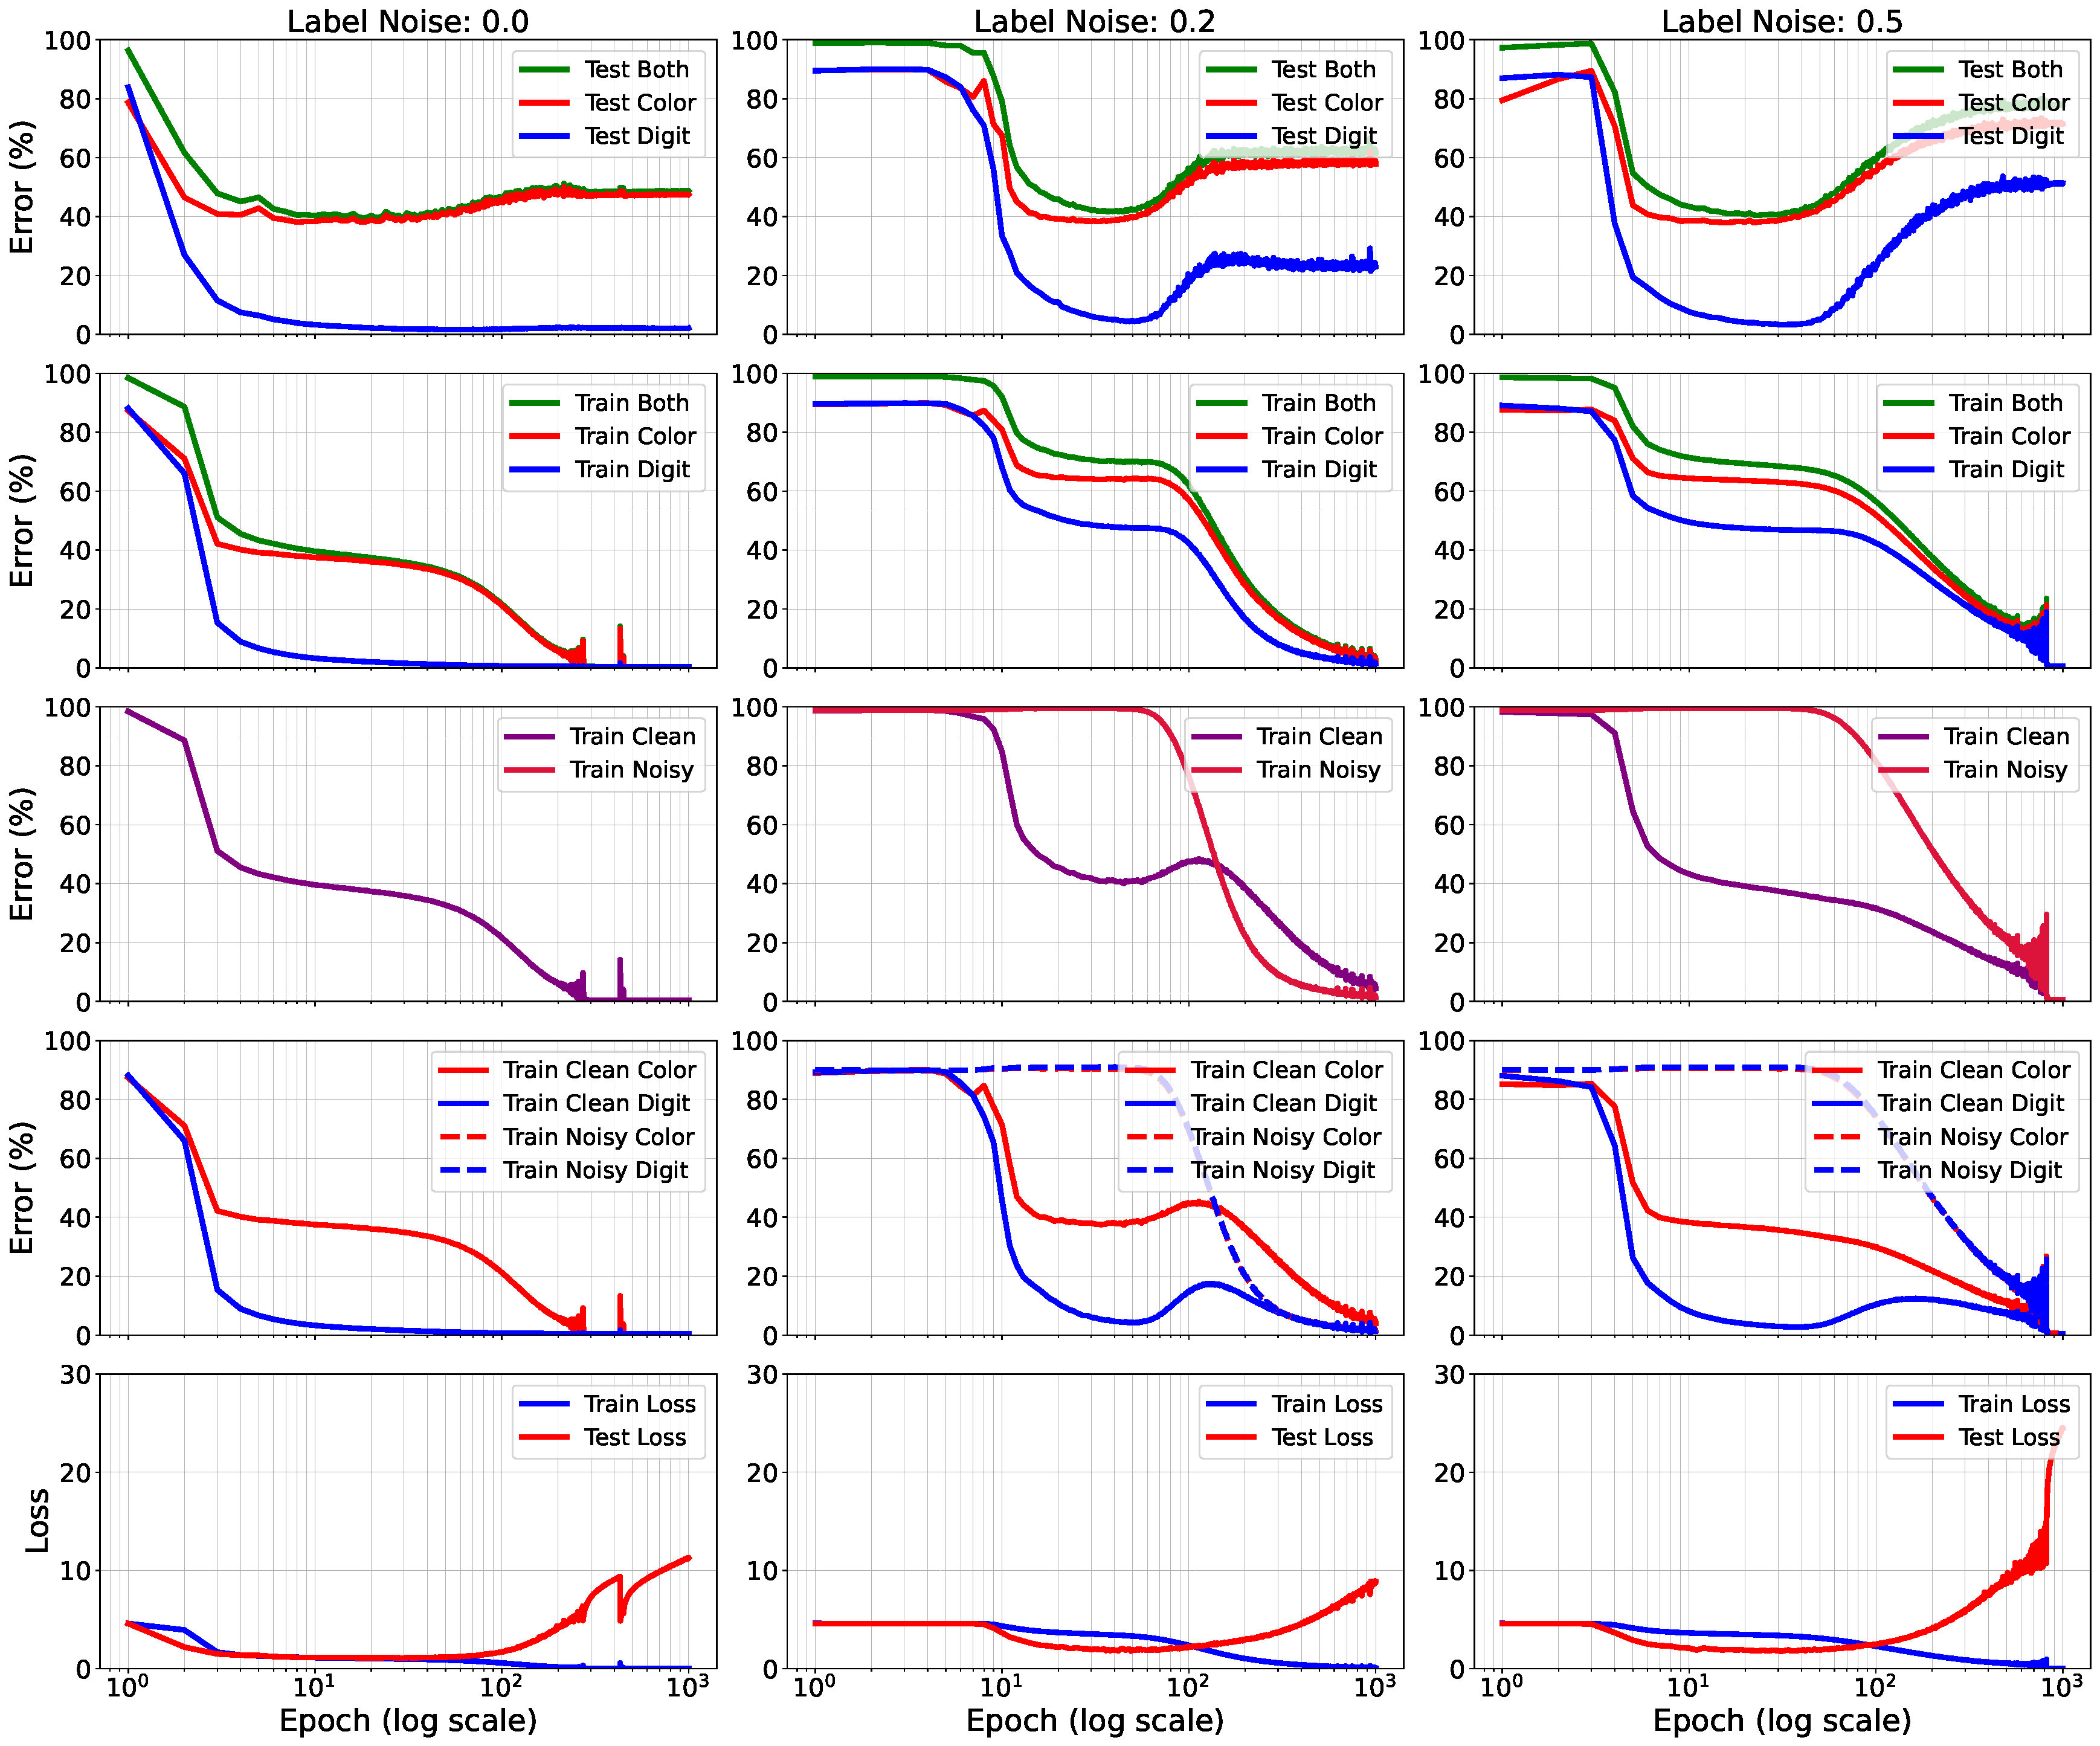
\includegraphics[width=\linewidth]{fig/erroe_metrics_by_variances/error_metrics_by_label_noise_variance_3612.pdf}
    \caption{$\sigma^2 = 10^{3.5}$のときのそれぞれのラベルノイズにおける結果}
    \label{fig:errors_by_label_noise_variance_3612}
\end{figure}

\begin{figure}[H]
    \centering
    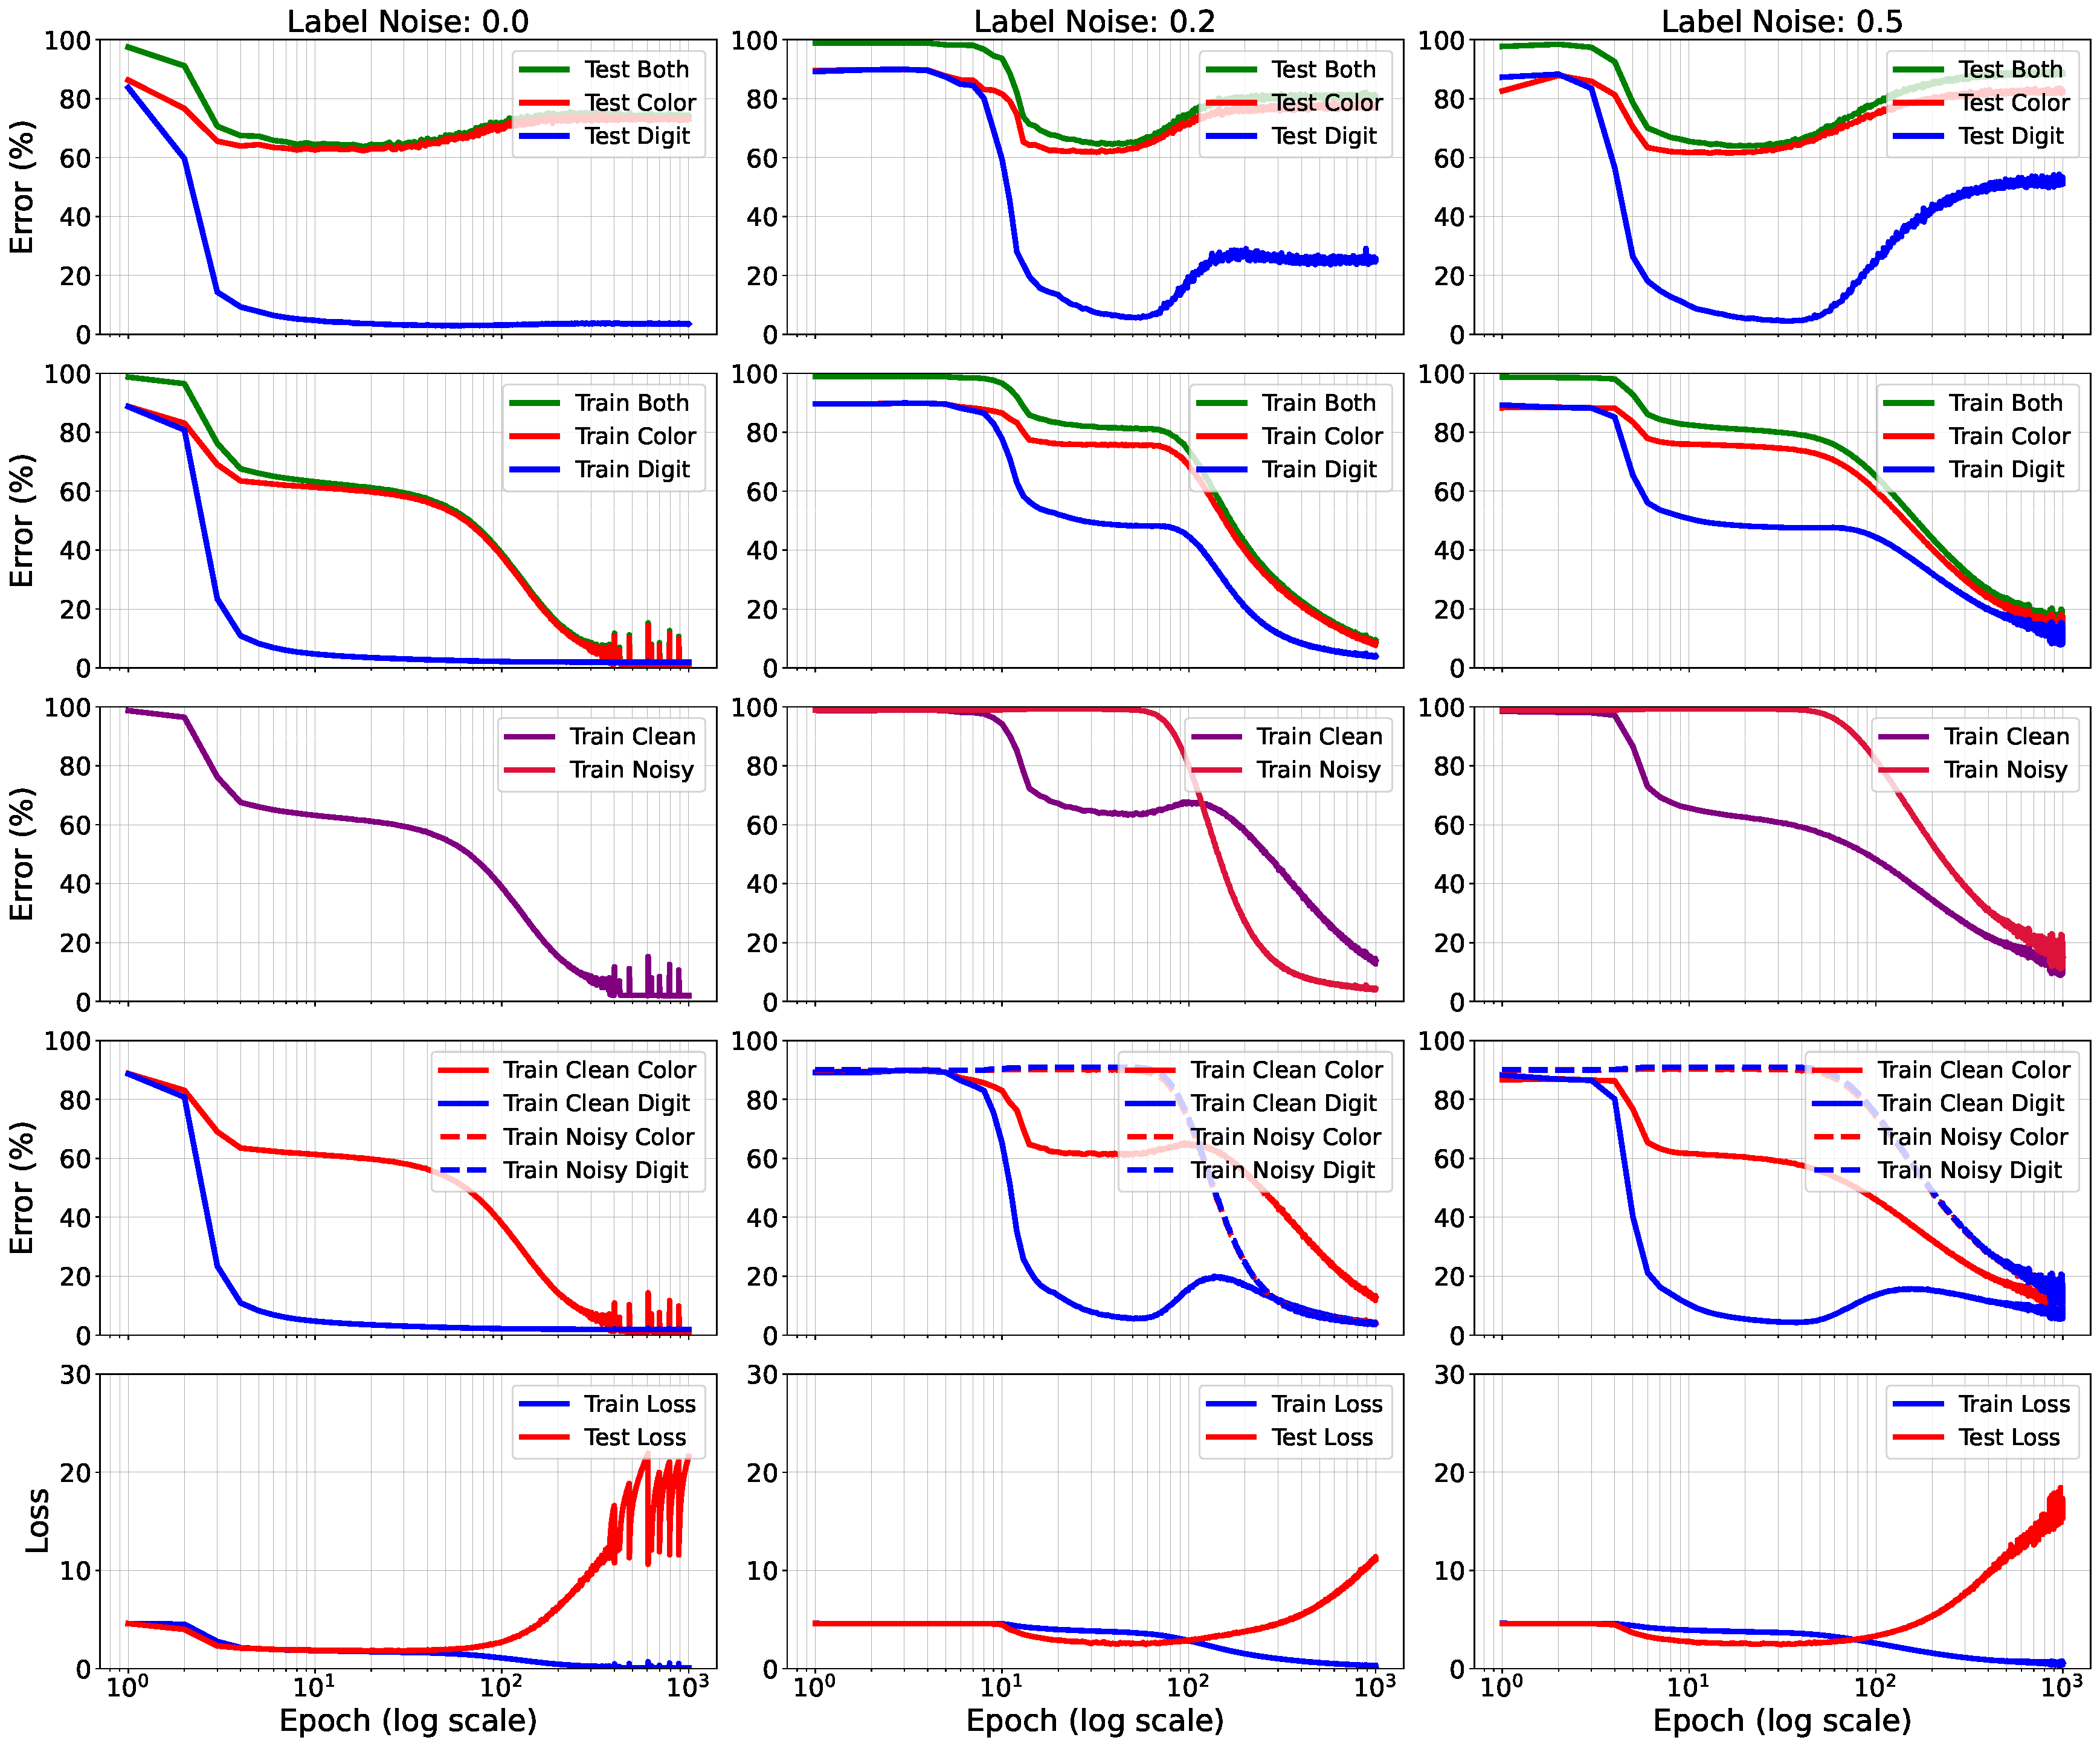
\includegraphics[width=\linewidth]{fig/erroe_metrics_by_variances/error_metrics_by_label_noise_variance_10000.pdf}
    \caption{$\sigma^2 = 10^4$のときのそれぞれのラベルノイズにおける結果}
    \label{fig:errors_by_label_noise_variance_10000}
\end{figure}

\begin{figure}
    \centering
    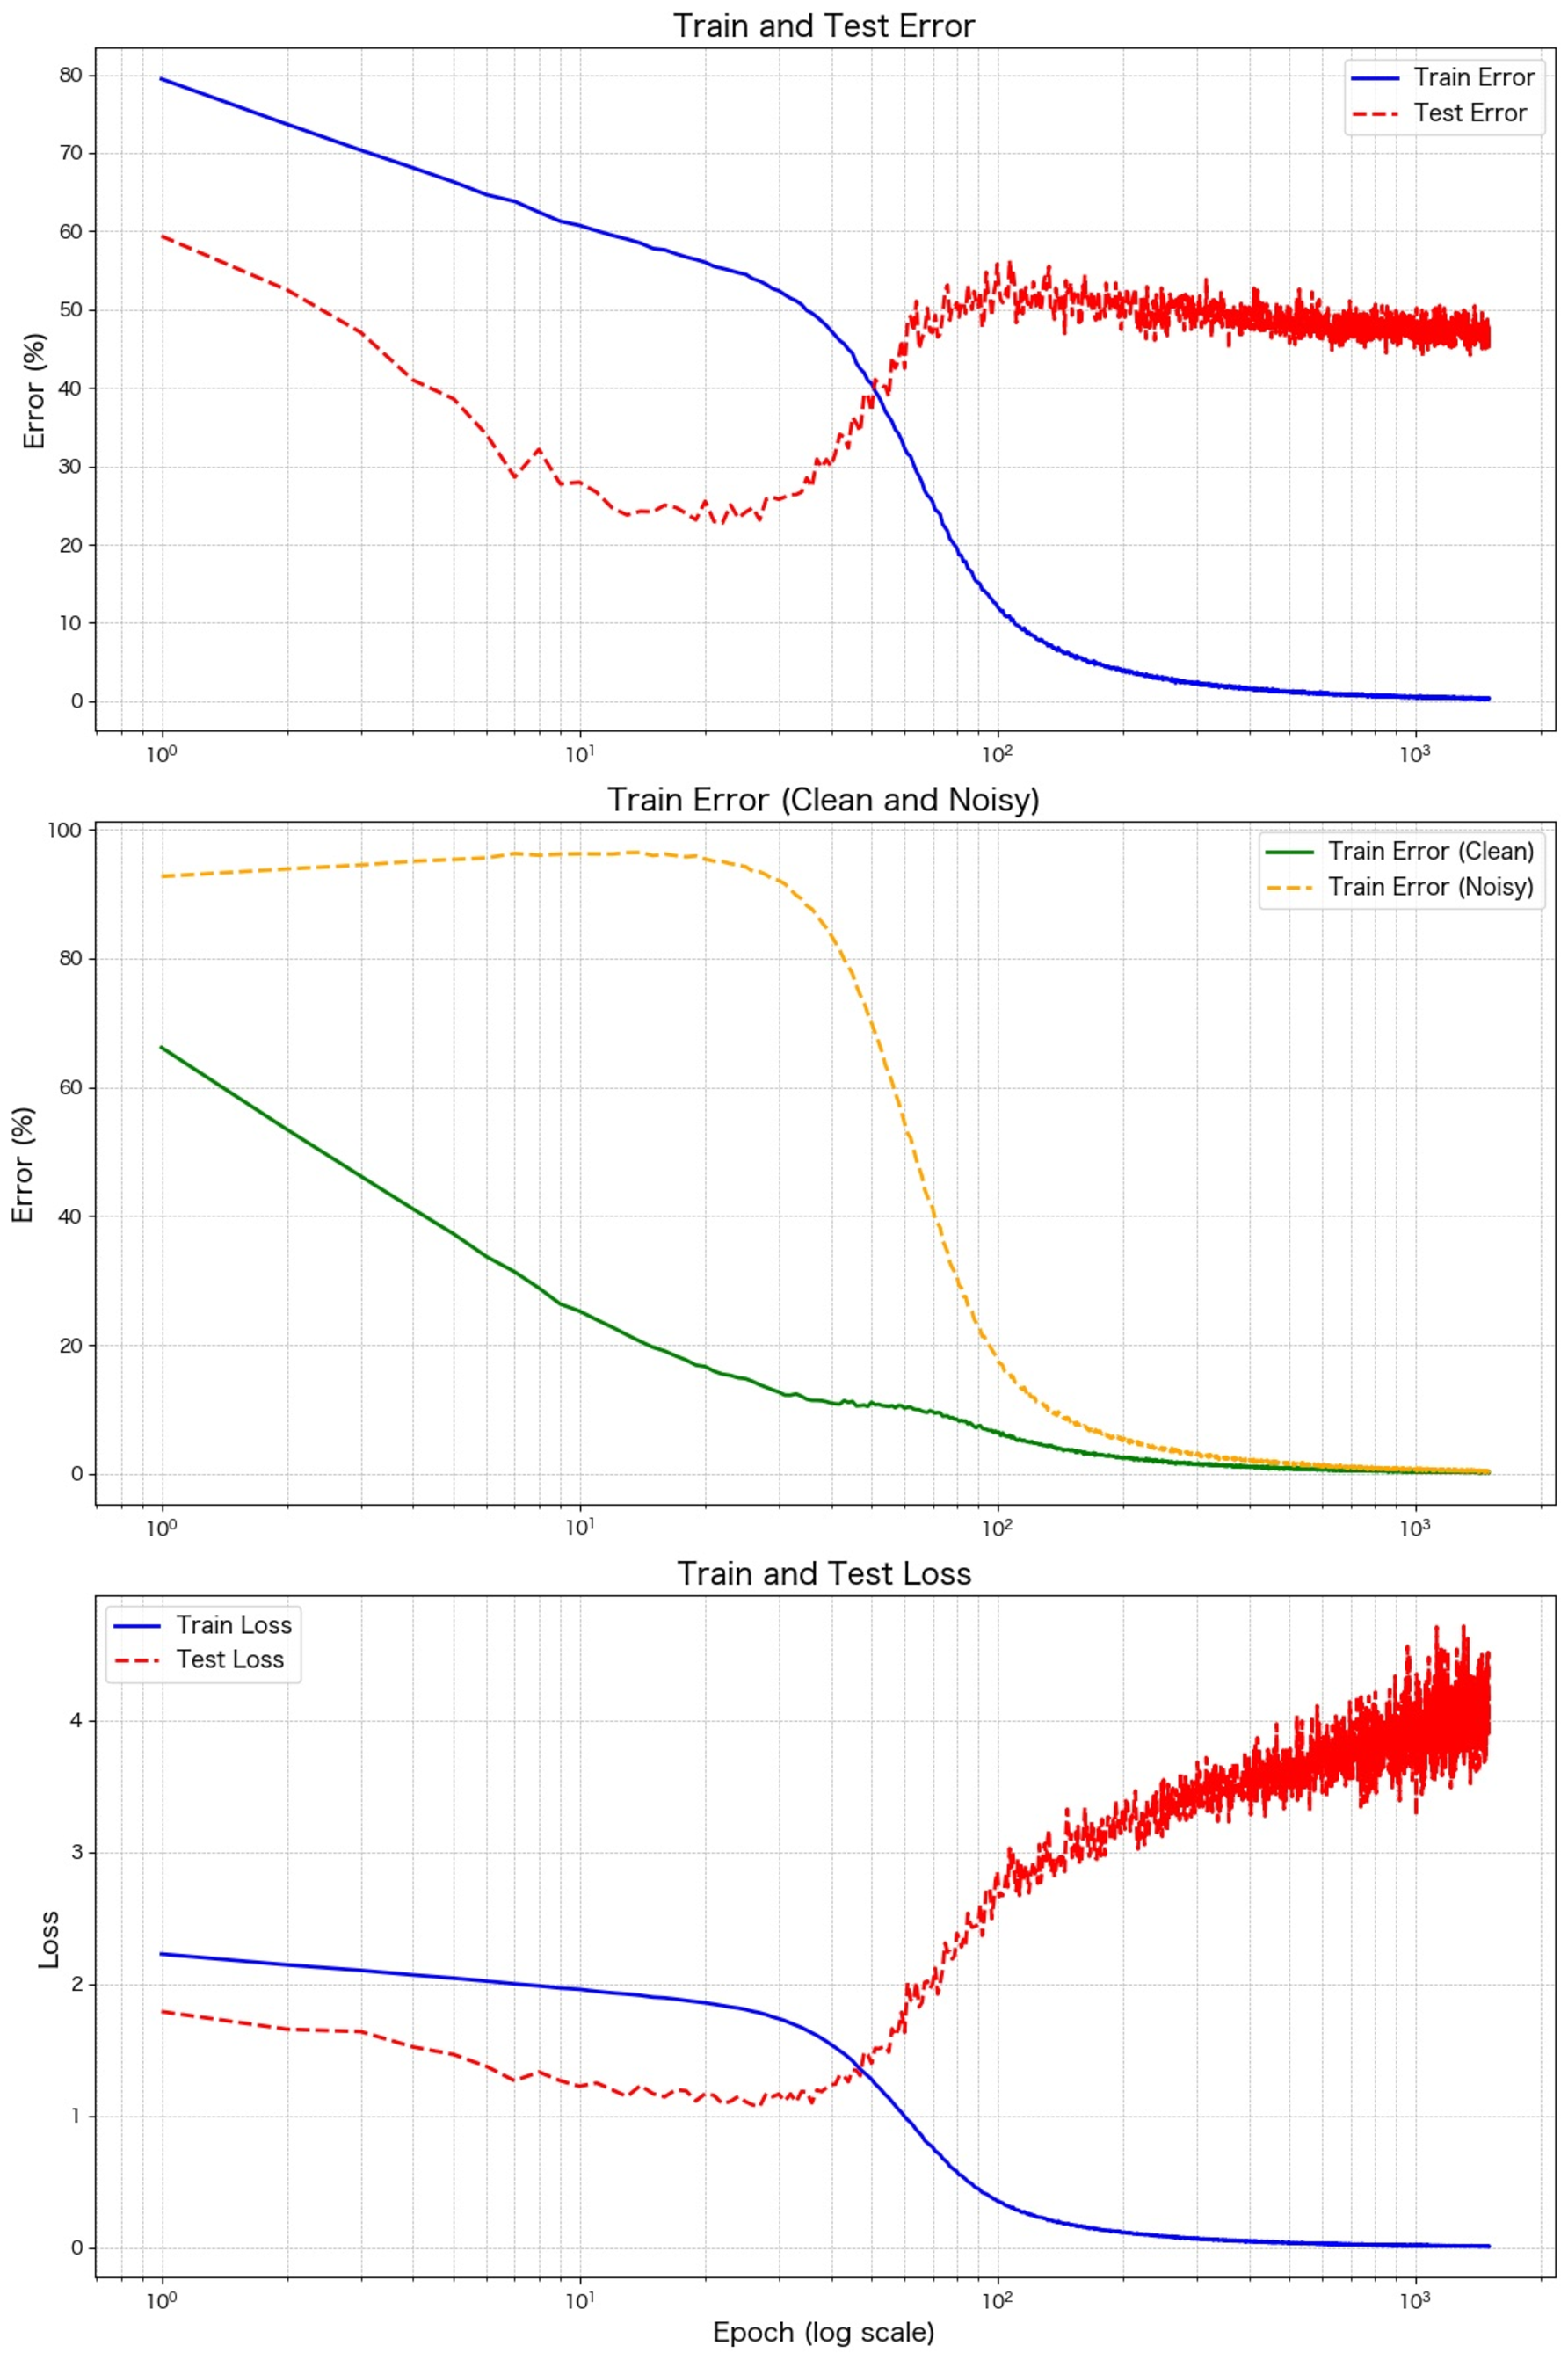
\includegraphics[width=\linewidth]{fig/nakkiran_resnet18_clean_noisy.pdf}
    \caption{Nakkiranの設定による,ラベルノイズあり・なしに分けた結果}
    \label{fig:nakkiran_resnet18_clean_noisy}
\end{figure}

\newpage

\subsection{モデルの層による変化}
8 層のCNN では,より深い層構造がもたらす効果が確認できる.図\ref{fig:5layer_results},図\ref{fig:8layer_results}
に$\gamma = 0.2,\sigma^2 = 0$の層による比較を示す.
Phase1 において,テスト誤り率はより遅いタイミングでに低下し始める.そして,5層のCNNに比べ,テスト誤り率の上昇が抑制された.
Phase3 においてはテスト誤り率の緩やかな上昇がさらに軽減される結果となった.また,8層のCNNでもラベルノイズなしデータに対して二重降下現象が観測されたが,
その程度は5 層のCNN よりも小さく,より安定した学習が行われたことが示唆される.

\begin{figure}[H]
    \centering
    \begin{minipage}[t]{0.48\linewidth}
        \centering
        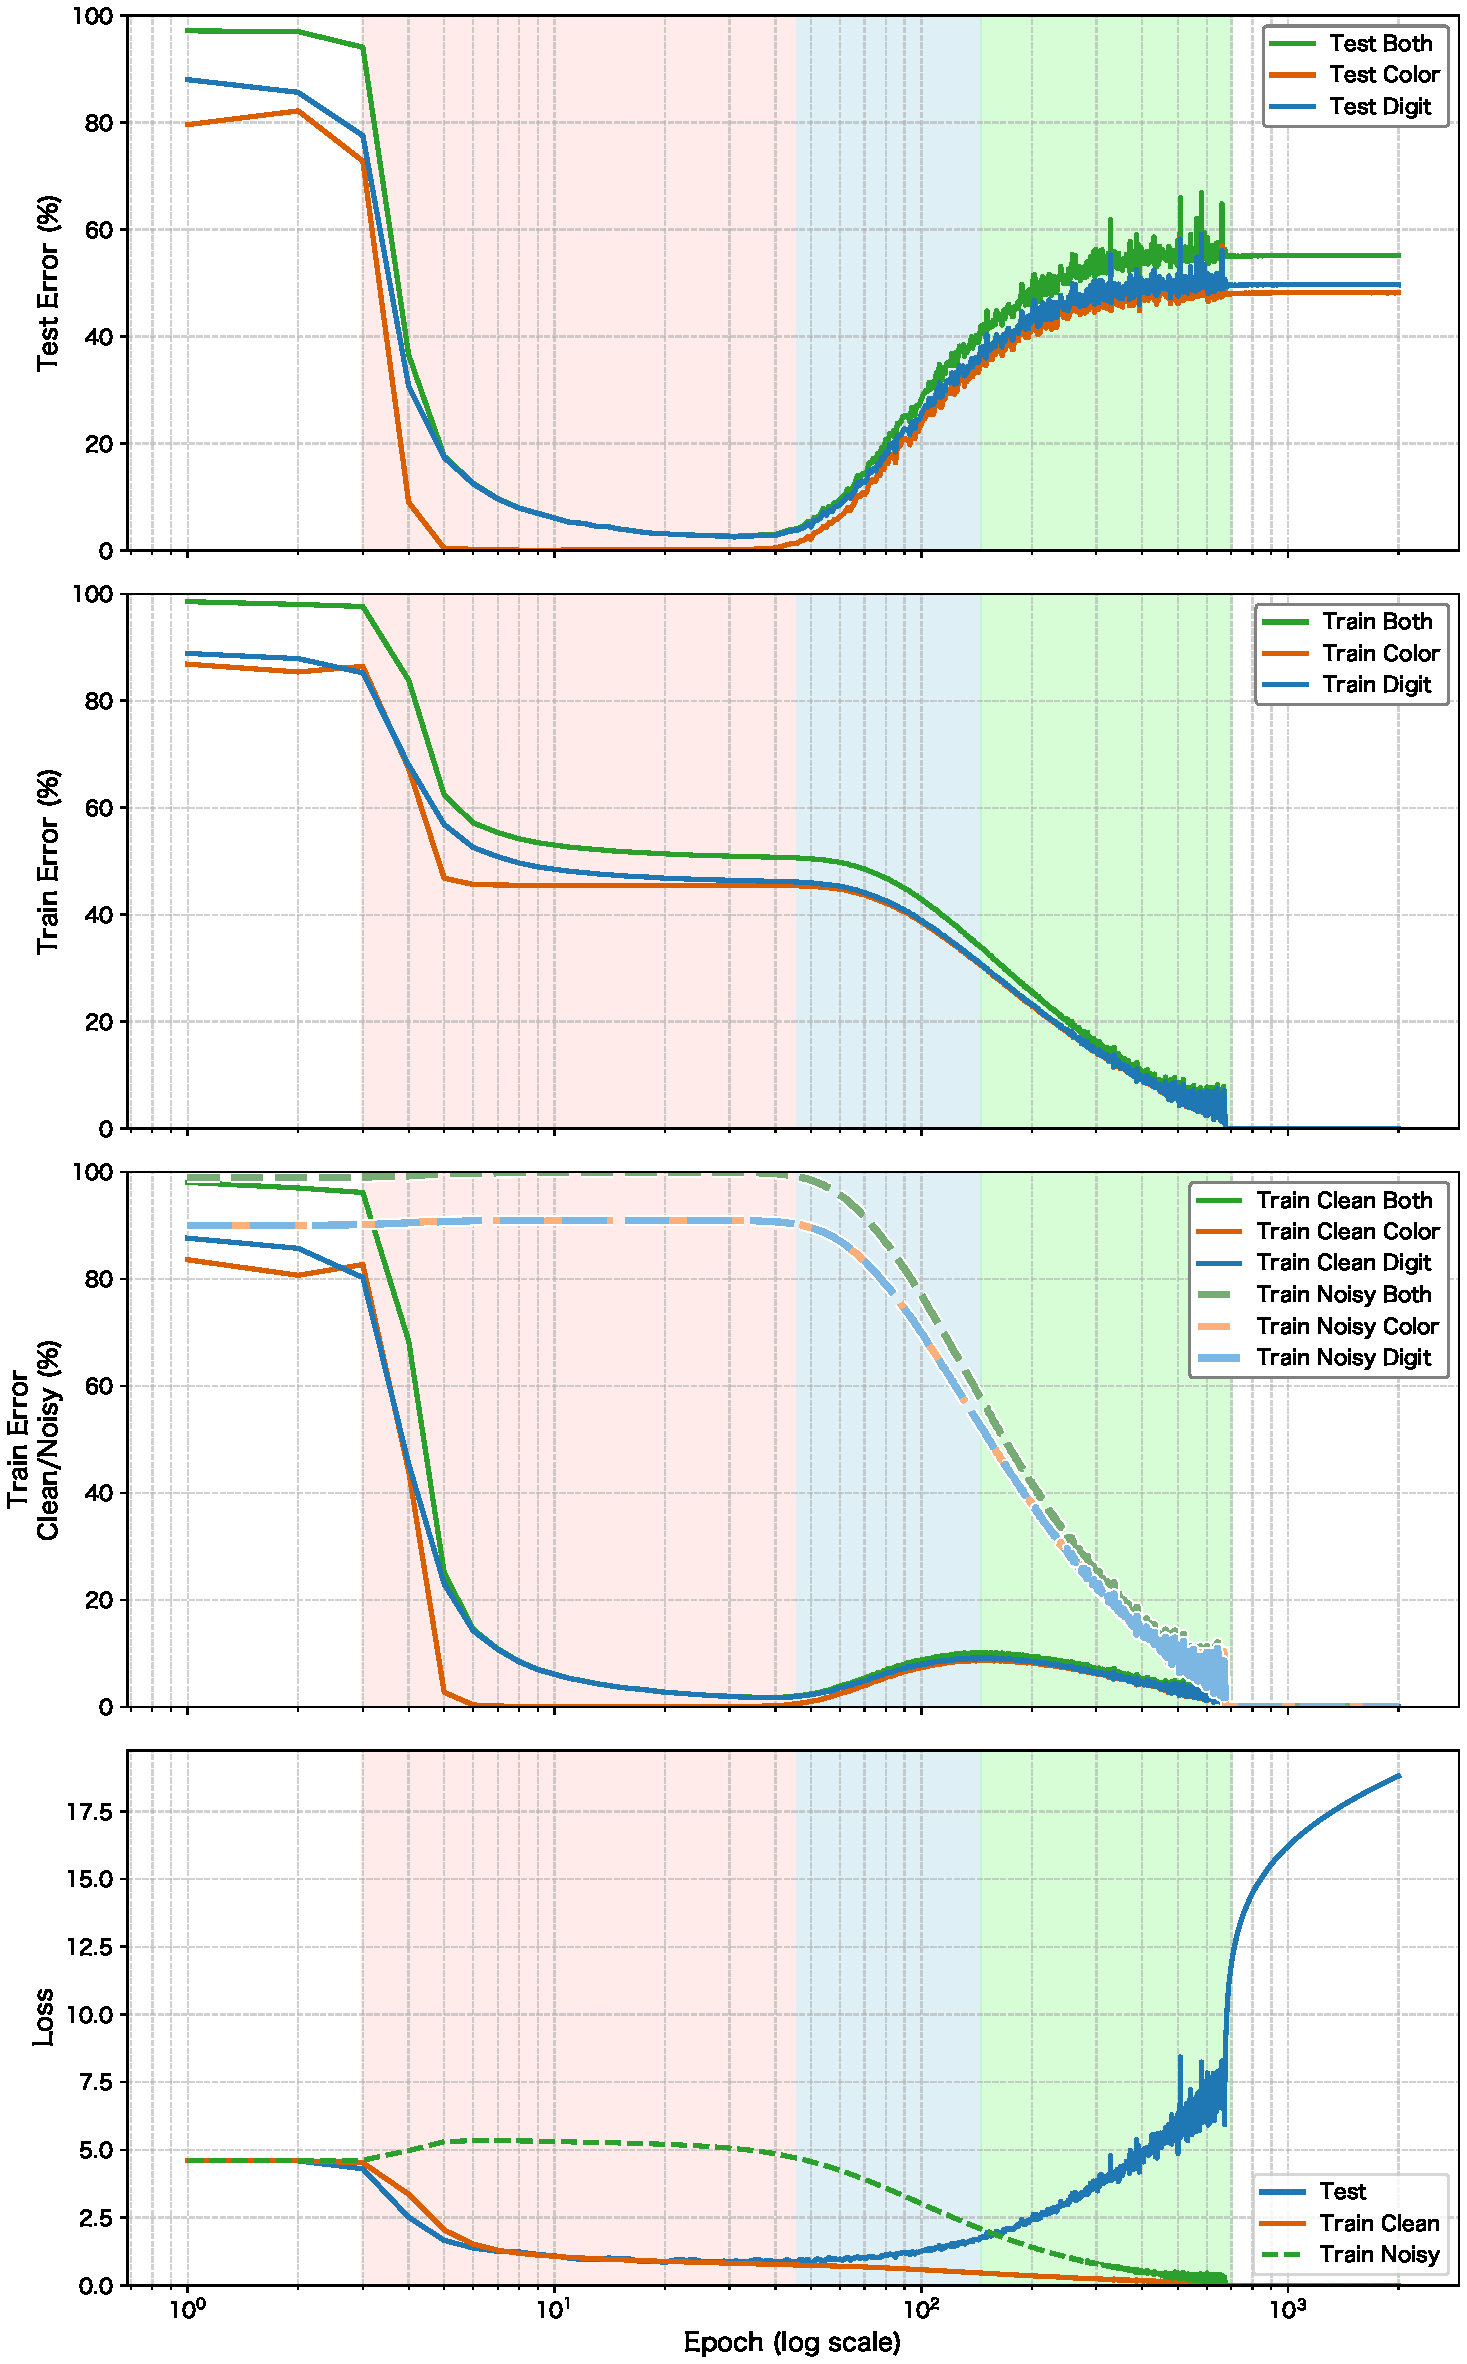
\includegraphics[width=\linewidth]{fig/layer_comparison/cnn5_error_comp_layer.pdf}
        \caption{5層のCNNモデルの100クラス分類タスクにおけるそれぞれの誤り率($\gamma = 0.5$)}
        \label{fig:5layer_results}
    \end{minipage}
    \hfill
    \begin{minipage}[t]{0.48\linewidth}
        \centering
        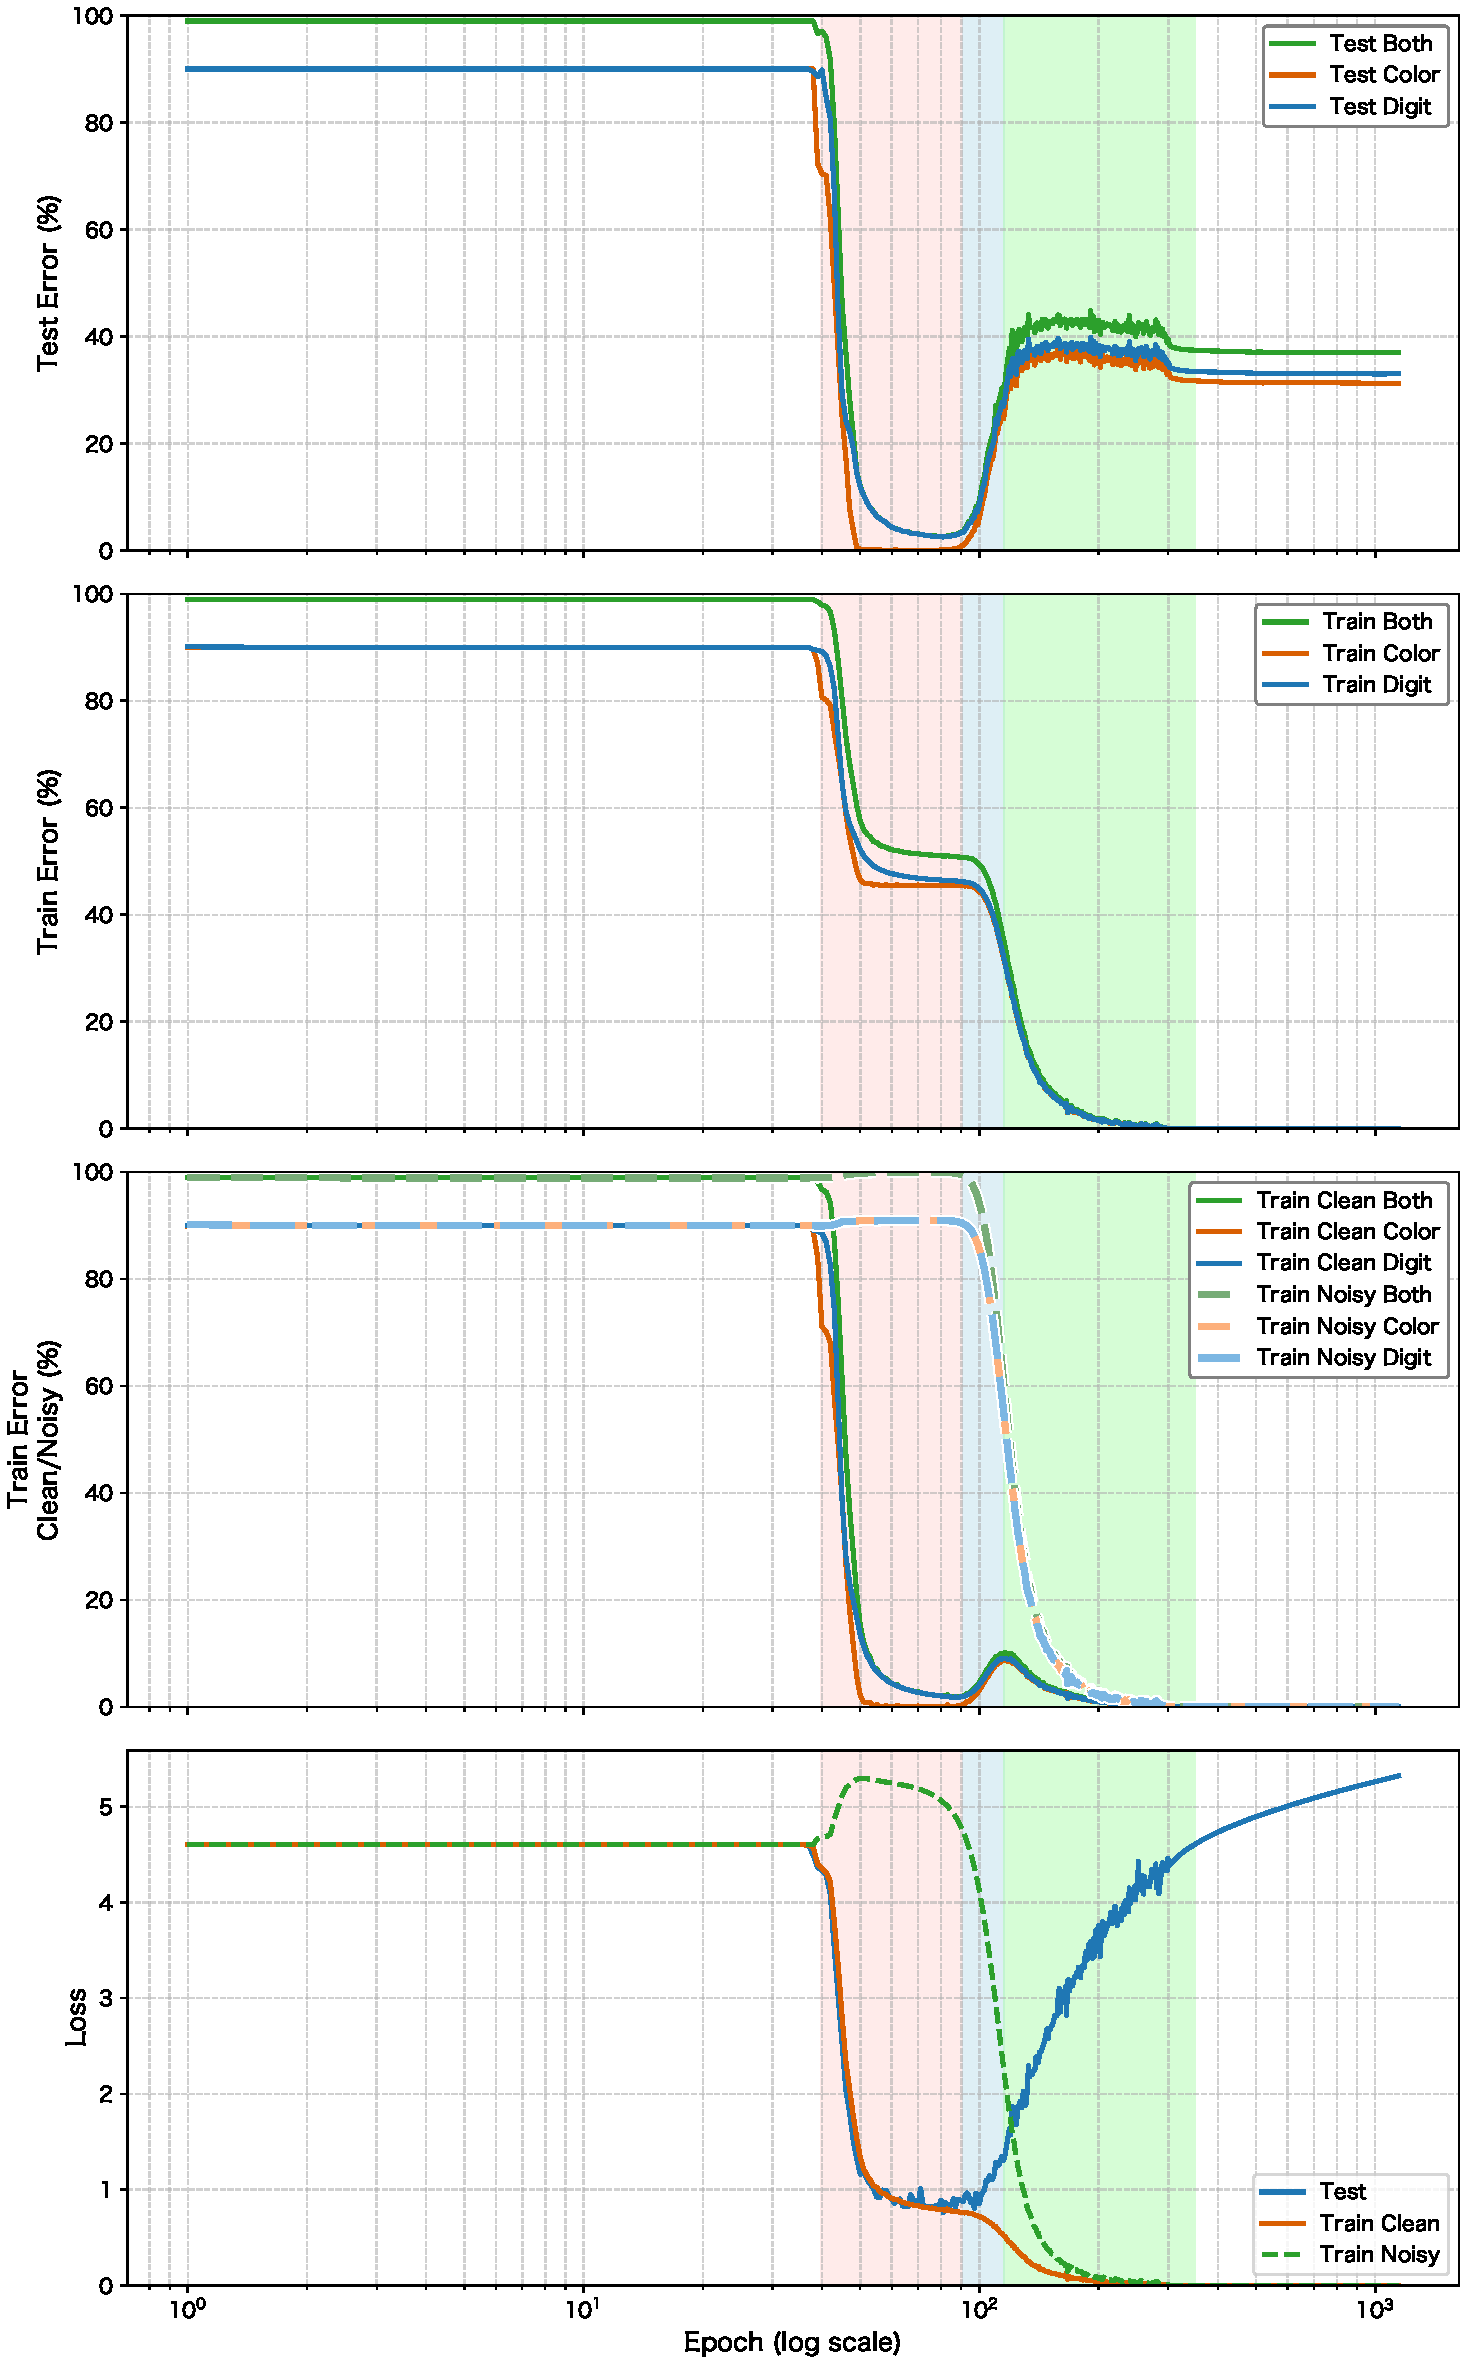
\includegraphics[width=\linewidth]{fig/layer_comparison/cnn8_error_comp_layer.pdf}
        \caption{8層のCNNモデルの100クラス分類タスクにおけるそれぞれの誤り率($\gamma = 0.5$)}
        \label{fig:8layer_results}
    \end{minipage}
\end{figure}

また,図\ref{fig:cnn_layers_comparison}に2,3,5,8,16層のCNNモデルのそれぞれの誤り率を示す.
CNNモデルの層数による性能評価の実験結果について,以下の重要な知見が得られた.

2層モデルは,学習の初期段階で比較的速い誤差の減少を示したものの,最終的な性能は他のモデルと比較して限定的であった.
特に,訓練エラー率とテストエラー率の両方において約\SI{40}{\percent}程度で停滞し,モデルの表現力の限界を示唆する結果となった.
3層モデルは2層モデルと同様に,早期の学習段階でエラー率の減少を示したが,最終的なエラー率は約\SI{30}{\percent}付近で収束した.
このことは,層数の微増による性能向上の効果が限定的であることを示している.
5層と8層のモデルは,比較的早い段階(10エポック付近)でエラー率が\SI{20}{\percent}以下まで低下し,安定した学習を示した.
特に8層モデルは,色と数字の両タスクにおいて最も安定した学習を示し,最終的な誤差も比較的低い水準で収束した.
16層モデルは特徴的な学習パターンを示した.学習の初期段階($10^2$エポック以前)では誤差の改善がほとんど見られず,その後急激な性能向上を示すという段階的な学習曲線を描いた.
また,学習後期($10^3$エポック以降)では損失値の大きな振動が観察され,過学習の傾向が最も顕著であった.
さらに,ノイズを含むデータに対する性能低下が他のモデルと比較して著しく,モデルの深さと頑健性のトレードオフが明確に表れる結果となった.
この実験結果から,単純にモデルの層を深くすることが必ずしも性能向上につながるわけではなく,タスクの複雑さに応じて適切な層数を選択することの重要性が示唆された.

\newpage

\begin{figure}[H]
    \centering
    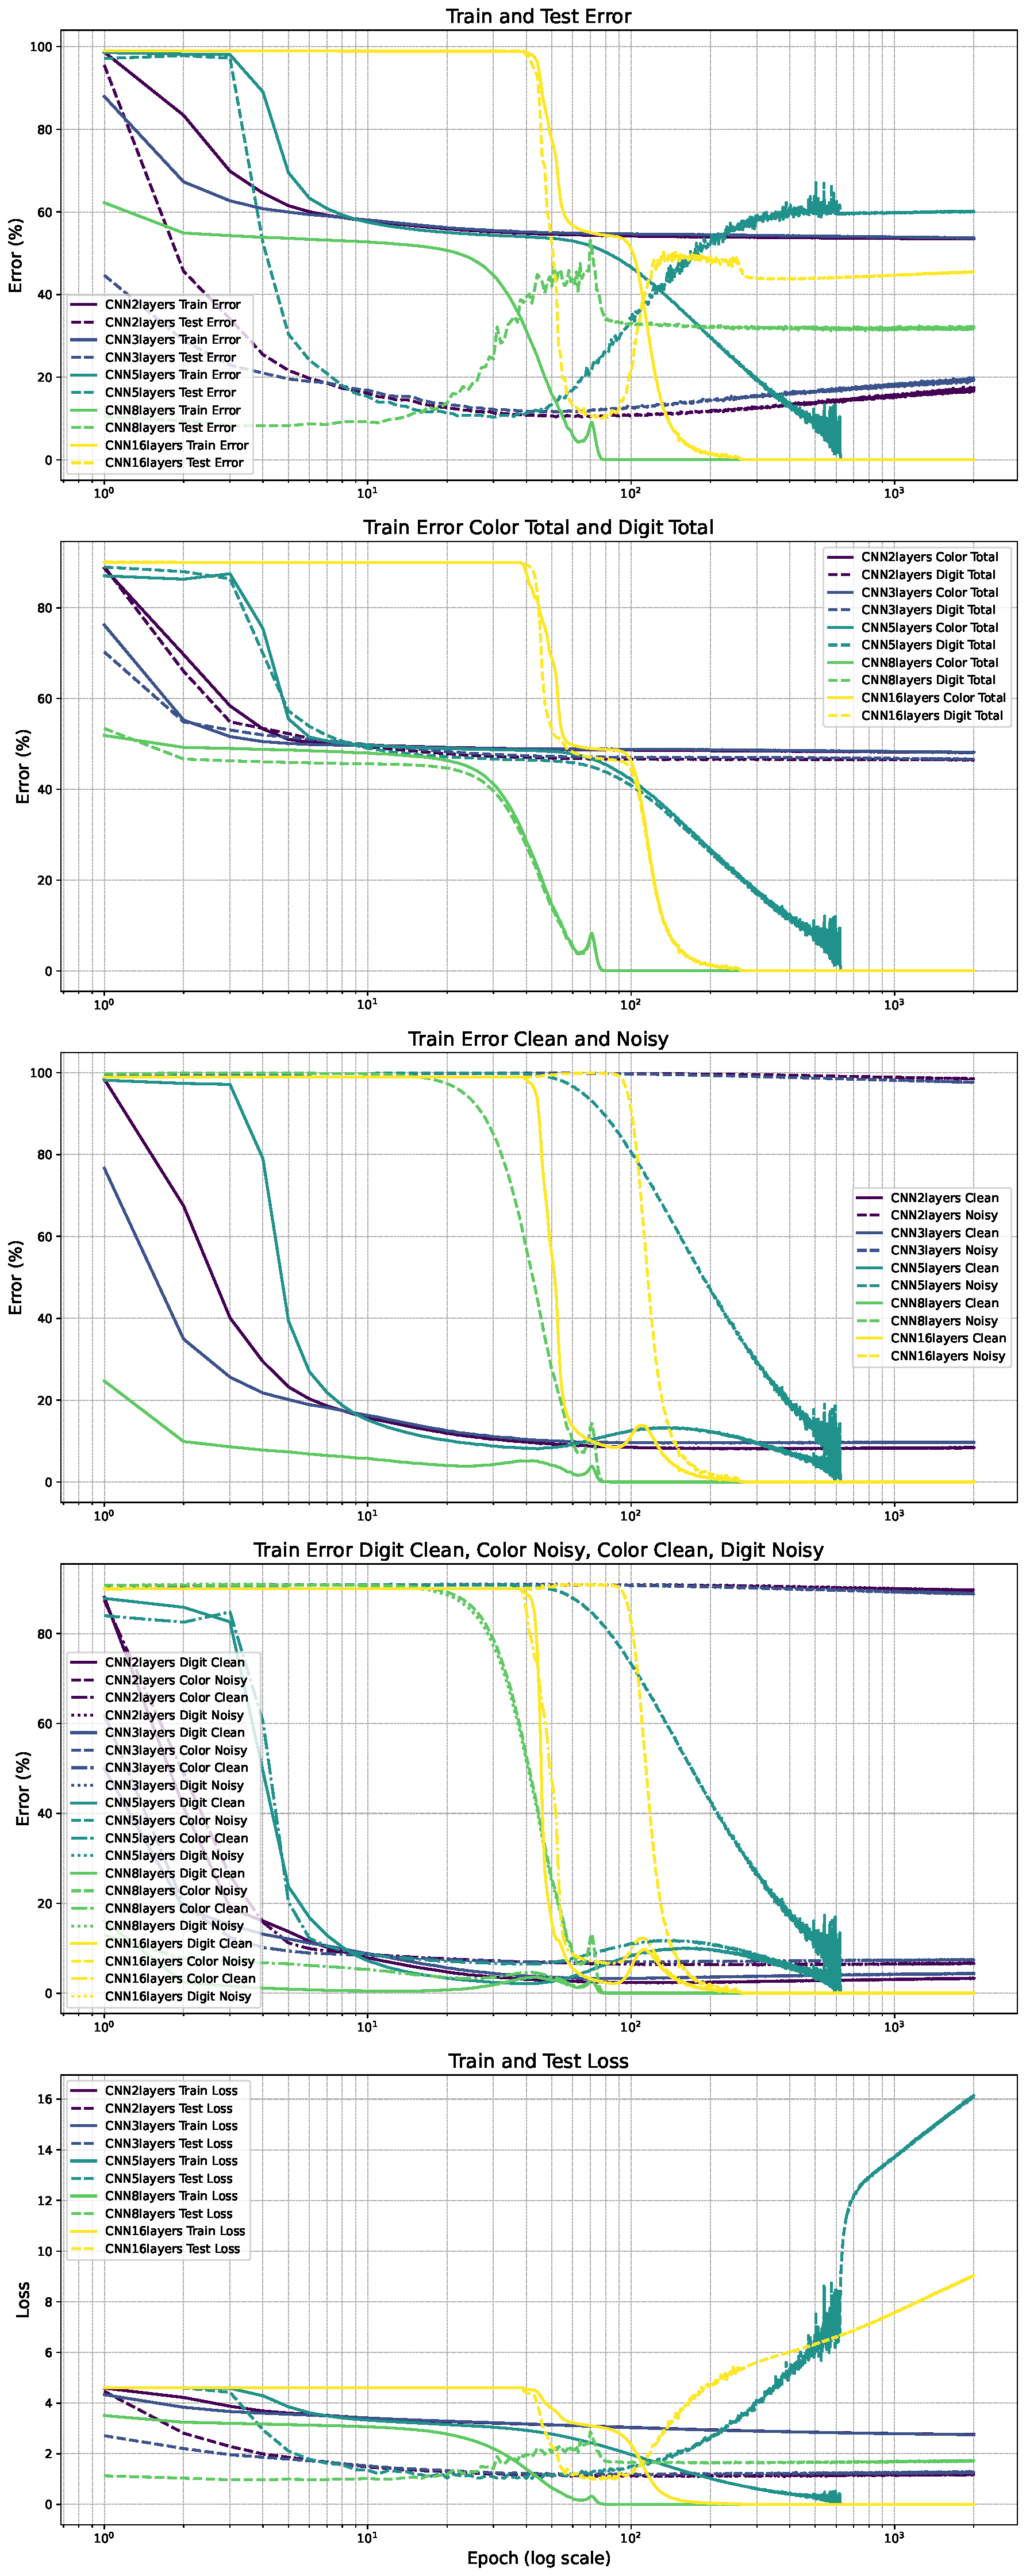
\includegraphics[width=0.6\linewidth]{fig/layer_comparison/cnn_layers_comparison.pdf}
    \caption{$\gamma = 0.5, \sigma^2 = 10^3$,のときのCNNの層の深さによる比較}
    \label{fig:cnn_layers_comparison}
\end{figure}

\newpage

\subsection{モデル幅による変化}

CNNのチャネル幅(Width)がモデルの性能に与える影響について,以下の実験結果が得られた.
結果を図\ref{fig:modelwidth_ln02}に示す.

Width 1のモデルは,訓練エラー率とテストエラー率の両方において,学習の収束が最も遅く,
最終的なテストエラー率も約\SI{20}{\percent}と高い値を示した.
特筆すべき点として,$10^2$エポック以降で訓練エラー率が\SI{0}{\percent}近くまで減少する一方で,
テストエラー率は高止まりしており,早期の段階で過学習が発生していることが確認された.
これは,チャネル幅が狭すぎることによるモデルの表現力の不足を示唆している.興味深いことに,カラー情報のノイズに対して特に脆弱性を示したが,
これはチャネル幅の狭さにより色空間の複雑な特徴を十分に捉えられていないことが原因として考えられる.

Width 2およびWidth 4のモデルは,10エポック付近から徐々に性能が向上し始め,
最終的なテストエラー率は\SI{10}{\percent}程度まで改善した.Width 1と比較すると過学習の発生が遅く,
特にWidth 4のモデルは,カラー情報と数字情報の両タスクにおいて安定した学習を示した.しかしながら,
$10^2$エポック以降では,これらのモデルにおいても訓練エラー率とテストエラー率の乖離が徐々に大きくなり,
緩やかな過学習の傾向が観察された.特に注目すべき点として,Width 4モデルではノイズの有無による性能差がWidth 2モデルより小さく,
これはチャネル幅の拡大がモデルの特徴抽出能力を向上させることを示唆している.

Width 8のモデルは,最も早い段階(1エポック付近)から急速な性能向上を示し,
最終的なテストエラー率は\SI{5}{\percent}未満という最も優れた性能を達成した.
また,訓練ロスとテストロスの推移も安定しており,他のモデルと比較して過学習の傾向が最も抑制されていることが確認された.
これは,適切なチャネル幅が,モデルの表現力と汎化性能のバランスを最適化できることを示唆している.
さらに,Width 8モデルは学習の初期段階における損失の減少が最も急峻であり,
これは十分な幅を持つチャネルが効率的な特徴学習を可能にすることを示している.
ノイズの影響に関する分析では,チャネル幅が広いモデルほどノイズに対する頑健性が高いことが示された.
特にWidth 8のモデルは,ノイズを含むデータに対しても安定した性能を維持し,
クリーンなデータとノイズを含むデータの間のエラー率の差が最も小さかった.
特筆すべき点として,カラー情報のノイズに対する頑健性がWidth 8モデルで顕著に高く,
これは広いチャネル幅により,ノイズの影響を受けにくい堅牢な特徴表現を学習できていることを示唆している.
一方,Width 1のモデルでは,ノイズの有無によって大きな性能差が生じ,特にカラー情報のノイズに対して脆弱性を示した.
また,ノイズを含むデータセットでは,全てのモデルにおいて過学習の発生が早まる傾向が観察された.
数字認識タスクとカラー認識タスクの比較において,興味深い傾向が観察された.全てのモデルにおいて,
カラー認識タスクの方が数字認識タスクより高いエラー率を示す傾向があり,これは色空間の特徴抽出がより複雑な課題であることを示唆している.
特に,チャネル幅が狭いモデルほどこの傾向が顕著であり,カラー情報の効果的な処理には十分なチャネル幅が必要であることが明らかとなった.
これらの結果から,チャネル幅の拡大は,学習の収束速度,最終的な性能,過学習の抑制,およびノイズに対する頑健性の全ての面で有意な改善をもたらすことが示された.
特に,本実験で検証したパラメータの範囲では,Width 8が最適なチャネル幅であることが明らかとなった.さらに,タスクの複雑さとチャネル幅の関係性において,より複雑な特徴抽出を必要とするタスクほど,十分なチャネル幅が重要であることが示唆された.

\newpage

\begin{figure}[H]
    \centering
    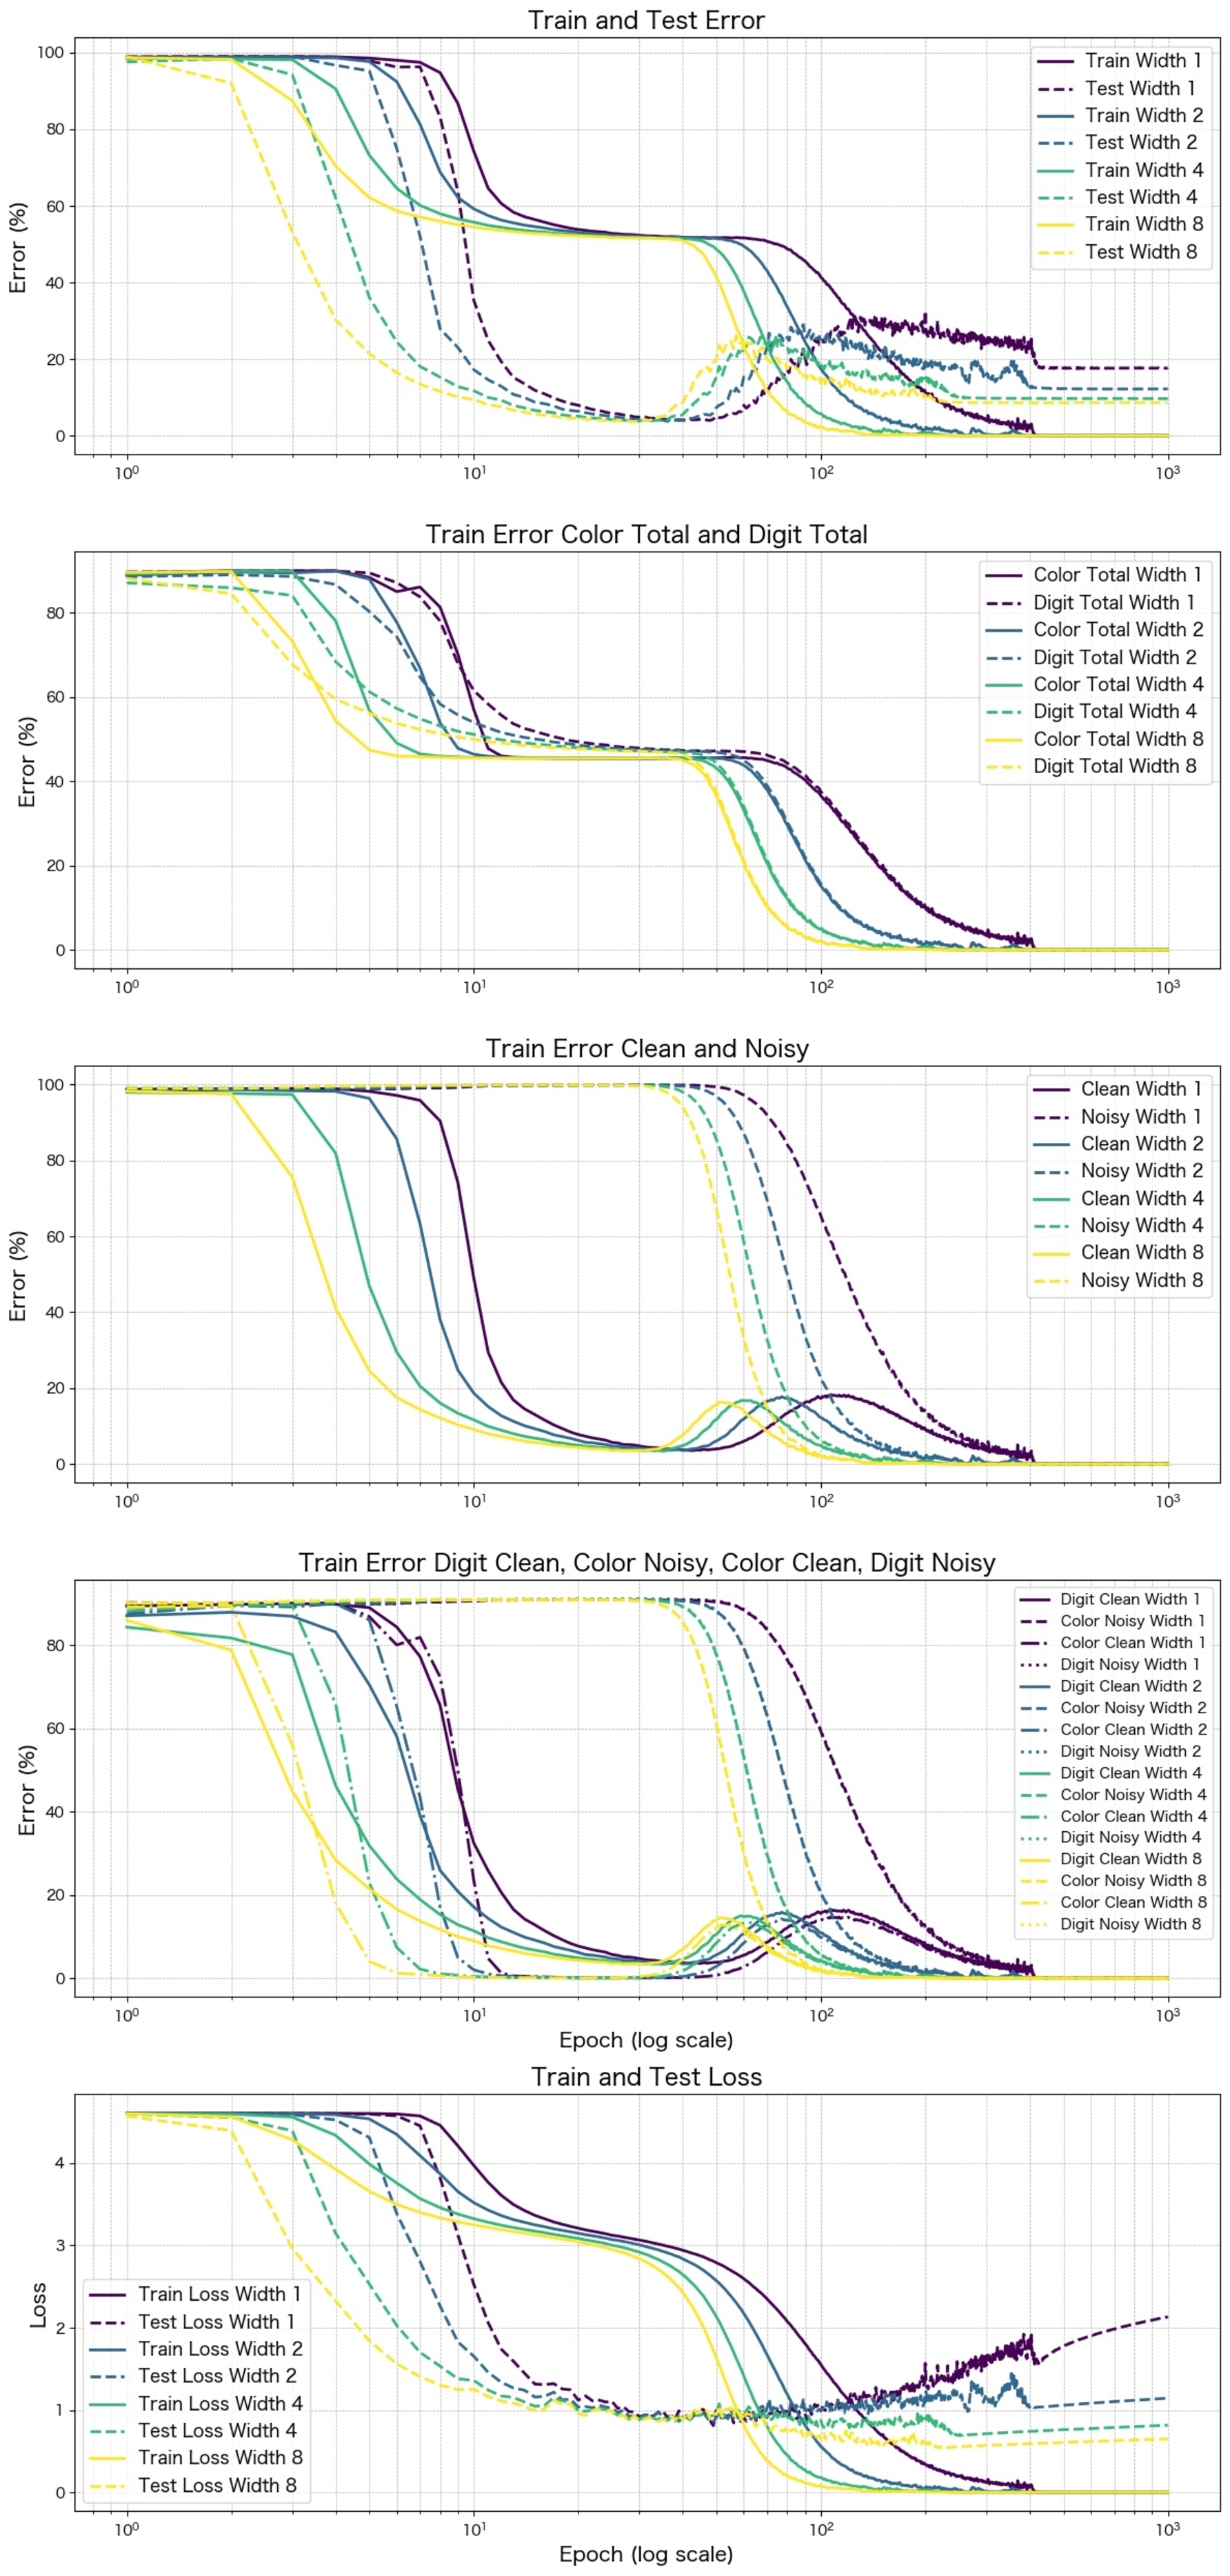
\includegraphics[width=0.7\linewidth]{fig/modelwidth_ln0.2.pdf}
    \caption{$\gamma = 0.2, \sigma^2 = 0$,のときのmodel width別の結果}
    \label{fig:modelwidth_ln02}
\end{figure}

\newpage

\subsection{チャネル幅とエポック数によるテストエラー率の分析}
また,図\ref{fig:modelwidth_heatmap}にエポックとチャネル幅の関係を表すヒートマップ示す.
テストエラー率のヒートマップ分析から,モデルのチャネル幅とエポック数の関係性について,以下の重要な知見が得られた.
チャネル幅8のモデルは,最も効率的な学習挙動を示した.具体的には,エポック10付近から急速にテストエラー率が低下し,
その後も安定して低いエラー率(約\SI{20}{\percent})を維持している.
これは,十分な表現力を持つチャネル幅の設定により,効率的な特徴抽出が可能となったことを示している.
一方,チャネル幅1および2のモデルでは,初期の学習段階(エポック1-10)において高いテストエラー率(約\SI{80}{\percent})が継続し,その後の低下も緩やかである.
特にチャネル幅1の場合,エポック100以降でテストエラー率が再び上昇する傾向が観察された.
この結果は,チャネル幅が狭すぎる場合,モデルの表現力が制限され,複雑な特徴を適切に抽出できないことを示唆している.
チャネル幅4のモデルは,チャネル幅8のモデルと比較して学習の開始が遅く,エポック20付近からテストエラー率の低下が始まる.
しかしながら,一度学習が進行し始めると,比較的安定した性能を示すことが確認された.
この挙動は,中程度のチャネル幅でも,十分な学習時間が与えられれば適切な特徴表現を獲得できることを示している.
特筆すべき点として,全てのチャネル幅において,エポック10付近で急激な性能変化が観察された.
この現象は,モデルがこの時点で重要な特徴表現を獲得する転換点を迎えることを示唆している.
特に,チャネル幅8のモデルではこの変化が最も顕著であり,効率的な学習が実現されている.
また,エポック100以降の長期的な学習挙動においても,チャネル幅による違いが明確に表れている.
チャネル幅8のモデルは安定した低エラー率を維持する一方,他のチャネル幅では性能の変動や劣化が観察された.
この結果は,適切なチャネル幅の設定が,モデルの長期的な学習安定性において極めて重要であることを示している.
これらの知見から,本実験条件下では,チャネルの幅が広いほど,より効率的な学習開始,安定した性能維持,
および長期的な学習の安定性が実現されることが明らかとなった.この結果は,深層学習モデルの設計における重要な指針となり,特にチャネル幅の設定が学習性能に与える影響を定量的に示している.

\begin{figure}[H]
    \centering
    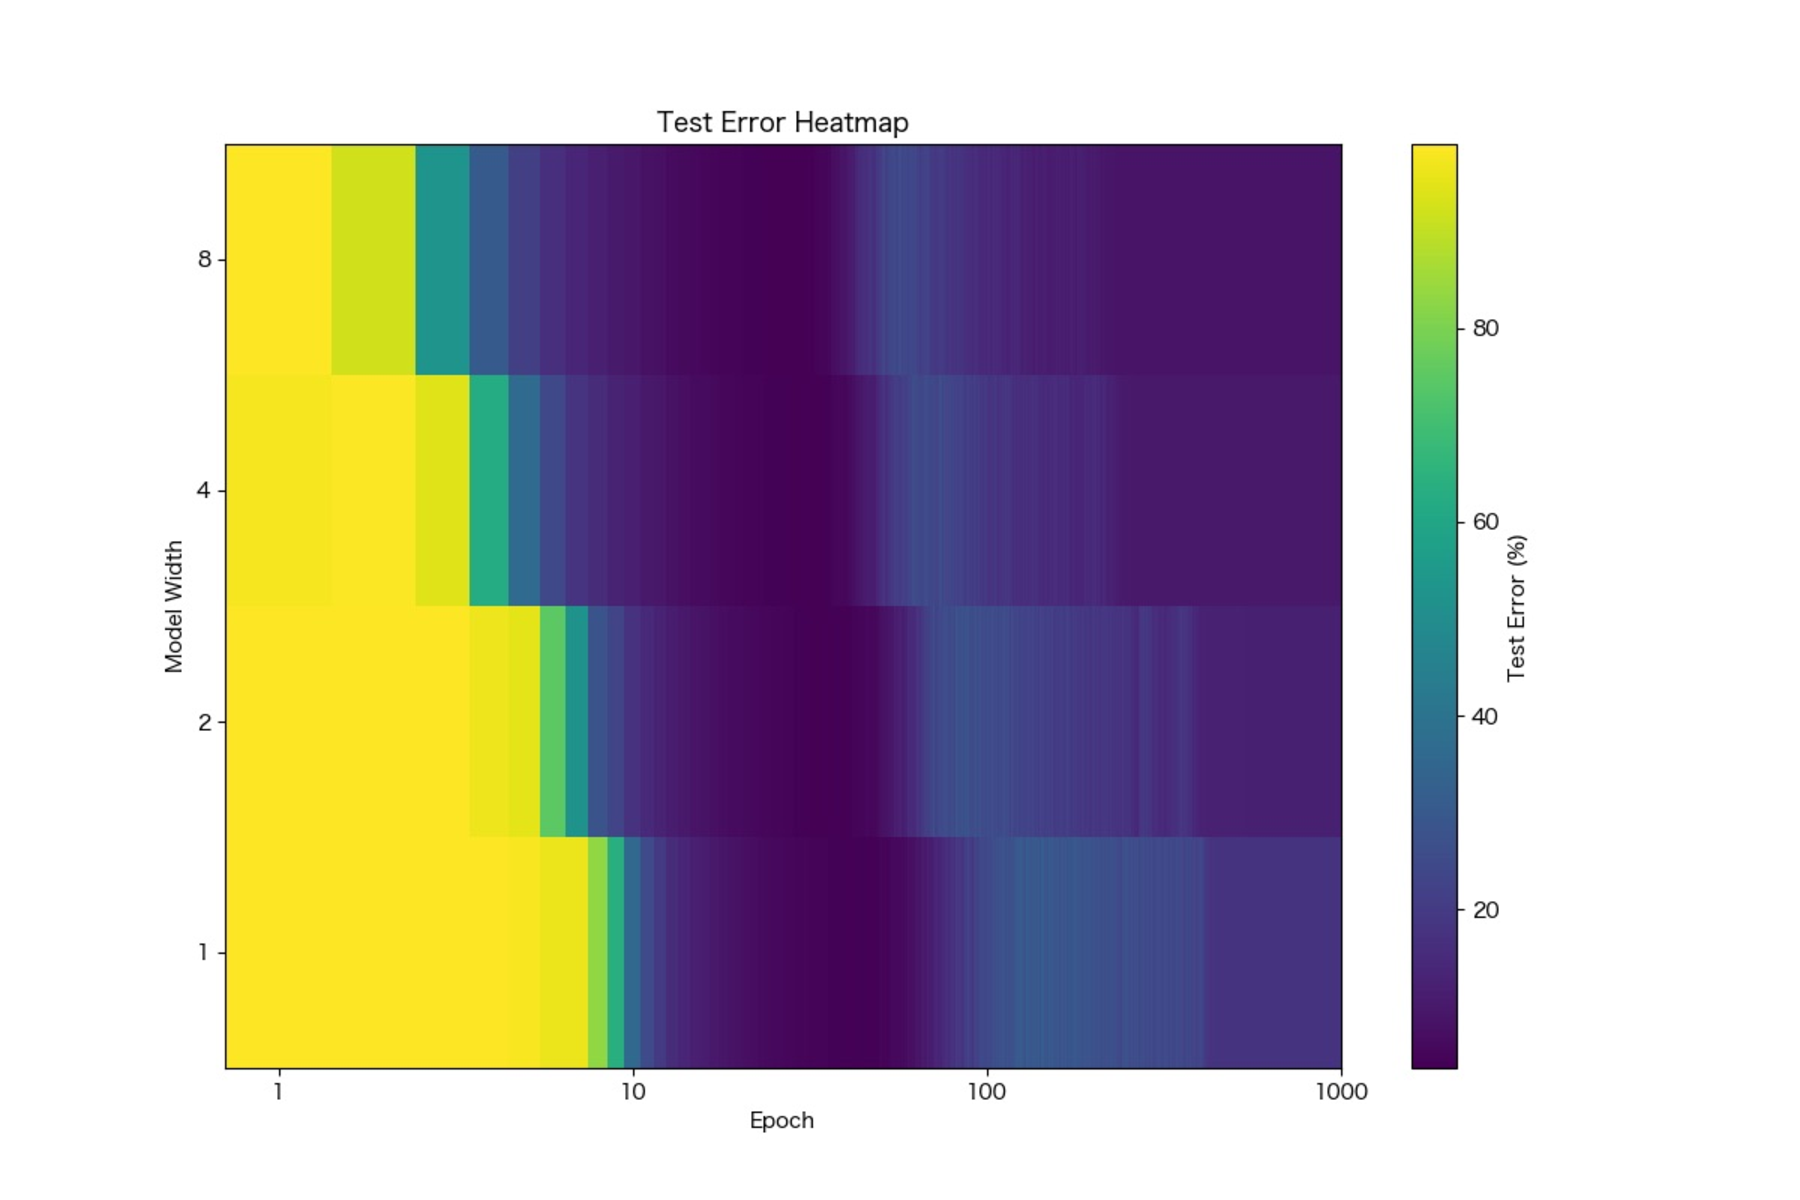
\includegraphics[width=\linewidth]{fig/test_error_heatmap_ln0.2.pdf}
    \caption[$\gamma = 0.2, \sigma^2 = 0$のときのEpochとModel Widthによるテストエラーのヒートマップ]{$\gamma = 0.2, \sigma^2 = 0$のときのEpochとModel Widthによるテストエラーのヒートマップ.
    モデルのチャネル幅が広くなると,過学習が早く発生することが確認できる.エポック軸に見てみると,例えば,8エポック付近では,width wiseで二重降下現象が確認できる}
    \label{fig:modelwidth_heatmap}
\end{figure}

\newpage

\subsection{重み減衰を適応したときの影響}
本研究では,データセット中に含まれるノイズ付きのサンプル(noisy samples)とノイズのないサンプル(clean samples)で損失関数への寄与度を差別化するため,
\texttt{weight\_noisy} と \texttt{weight\_clean} という2つの重みを導入している.
具体的には,各バッチ内の \texttt{noisy} サンプルおよび \texttt{clean} サンプルに対して,以下に示すように損失値を再スケーリングすることで,
ノイズの影響をコントロールしつつクリーンなサンプルからの学習信号を最大限に活用するようにしている.

\[
\texttt{total\_weight} = \texttt{weight\_noisy} + \texttt{weight\_clean}
\]

\[
\texttt{weights[idx\_noisy]} \;=\; \frac{\texttt{weight\_noisy}}{\texttt{total\_weight}} \times 2,
\quad
\texttt{weights[idx\_clean]} \;=\; \frac{\texttt{weight\_clean}}{\texttt{total\_weight}} \times 2
\]

このように重みを調整することで,ノイズを含むサンプルが過大に影響することを抑制しながら,
クリーンなサンプルから得られる学習信号も十分に取り入れられるように工夫している.
これにより,ノイズによる学習の不安定化を緩和したときの影響を観察する.
その結果を図\ref{fig:weight_decay}に示す.

\begin{figure}[t]
    \centering
    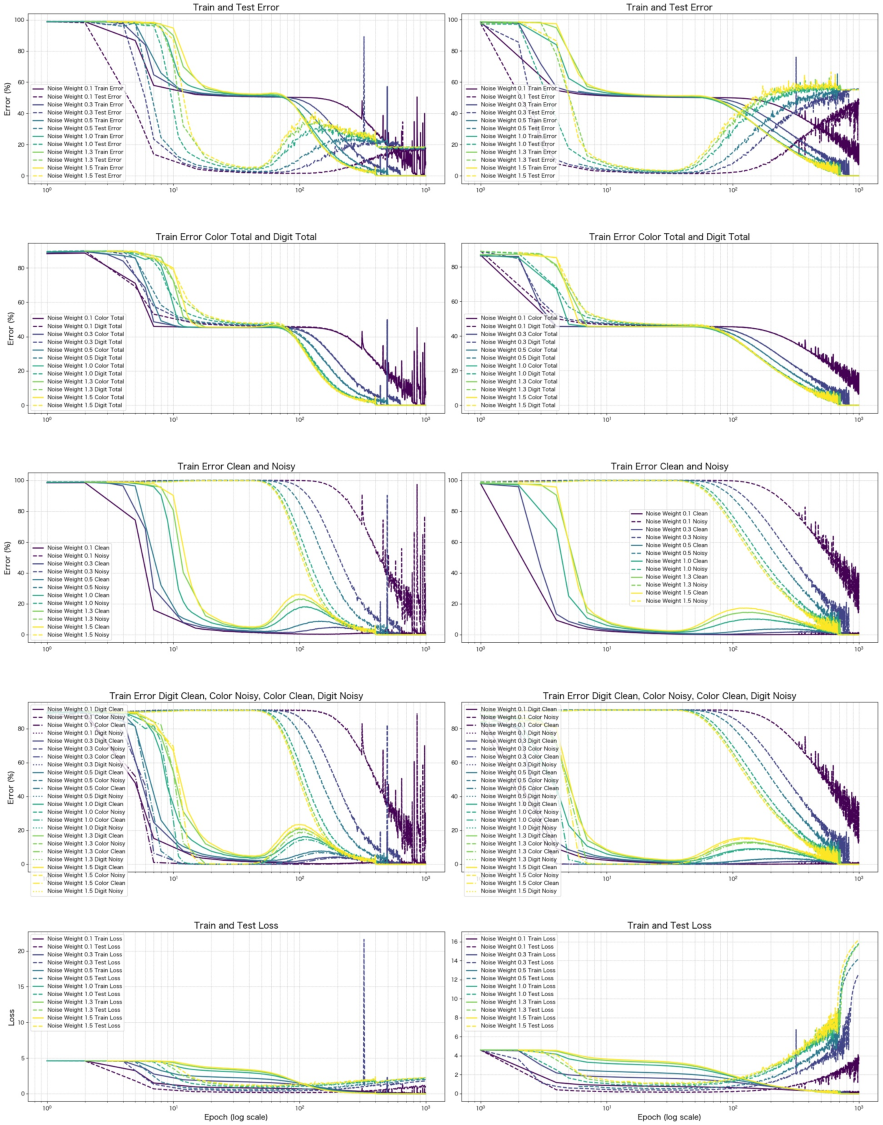
\includegraphics[width=\linewidth]{fig/weight_decay.pdf}
    \caption{重み減衰を適応したときの結果.左が$\gamma=0.2$、右が$\gamma=0.5$のときの結果.
    重み減衰を適応することで,ラベルノイズに対する頑健性が向上することが確認できる.}
    \label{fig:weight_decay}
\end{figure}


\chapter{考察}
まず,5層のCNNと8層のCNNの実験結果から,アーキテクチャの深さが概念獲得プロセスに本質的な影響を与えることが明らかとなった.
5層のCNNは8層のCNNと比較して,Phase1における色と数字の並列学習をより効率的に実現している.
この結果は,ネットワークの深さが増すことで,異なる視覚的特徴を同時に学習する能力が向上するが,
その学習が始まるためにより多くのニューロンが活性化しなければならないことを示唆している.
性能に関して,より深い層構造により,特徴抽出の階層性が高まり,色情報と形状情報を独立して処理できる表現空間が獲得されたためと考えられる.
特に興味深い点として,8層のCNNでは色と数字の認識精度が同期的に向上する傾向が観測された.
これは,より深い層構造が特徴の階層的な抽象化を促進し,複数の視覚的概念を効率的に並列処理できる表現を獲得できることを示している.
また,学習過程における二重降下現象の出現パターンがモデルの深さによって質的に異なることが観測された.
特に,8層のCNNはPhase2からPhase3への移行期において,CleanとNoisyの学習曲線が5層のCNNより早期に収束する傾向を示した.
この結果は,より深いアーキテクチャが,ノイズの影響を効果的に抑制しながら本質的な特徴を学習できることを示している.
さらに,この現象は従来の二重降下現象の研究では十分に説明されていなかった,アーキテクチャの深さと学習ダイナミクスの関係性に新たな知見を提供するものである.
色認識と数字認識の学習タイミングに関して,両モデルで顕著に異なる特性が観測された.
5層のCNNがPhase1において訓練データに対する色認識が50\%の正解率で停滞し始めるタイミングがより早い.
この結果は,ネットワークの表現能力が,概念獲得の時間的順序影響を与えることを示唆している.
特筆すべき点として,8層のCNNではPhase2における上昇が抑えられて,進行することが確認された.
これは,より深い層構造が,異なる視覚的特徴間の関係性を効果的に捉える能力を持つことを示していると考える.
次に,RGBノイズの分散を変化させた実験について考察する.$\sigma = 10\sqrt{10}$,$\sigma = 100$のノイズ条件下において,
色に対する難易度を上げても,ほとんど数字に対する誤り率の変化は見られなかった.
これは,CNNのモデル内部において,数字概念と色概念を分けて学習して,概念を獲得していることを示唆している.
本研究で観測された学習ダイナミクスは,従来のshape/texture biasの研究では捉えきれなかった重要な側面を明らかにした.
特に,明確に定義された概念(数字と色)を用いた分析アプローチにより,CNNの学習過程における概念獲得のメカニズムをより精緻に理解することが可能となった.
この知見は,今後の深層学習グモデルの設計において,層の深さと概念獲得能力の関係性を考慮する重要性を示唆している.
今後の研究課題として,より多様な視覚的概念や,異なる層構造を持つアーキテクチャでの検証が挙げられる.
また,本研究で観測された学習ダイナミクスの理論的な解明も重要な課題である.
これらの課題に取り組むことで,CNNの学習メカニズムのより深い理解と,より高度な視覚認識システムの実現が期待される.


\chapter{結論}

\chapter{今後の展望}

本研究の成果を踏まえ,今後の研究としてより複雑な視覚的概念への応用が考えられる.
例えば,テクスチャ,形状,物体の部分構造などの概念獲得メカニズムの解明が期待される.
また,異なるモダリティにおける概念獲得メカニズムの検証や,概念間の階層的な関係性の分析も重要な研究課題となる.

理論的な観点からは,概念獲得と表現学習の関係性の解明,二重降下現象と特徴表現の進化過程の数理的な理解,
最適なモデル設計のための理論的な指針の確立などが挙げられる.
これらの研究を通じて,効率的な転移学習手法の開発や解釈可能な人工知能システムの設計,
教師あり学習における教師信号の効率的な設計などへの応用が期待される.
さらに,概念獲得を促進する新しいネットワーク構造の提案や,
自己組織化による概念獲得メカニズムの研究,マルチタスク学習における効率的な特徴共有の実現なども重要な研究課題となる.
これらの研究の発展により,深層学習の基礎理論の確立と,より高度な人工知能システムの実現が期待される.


\appendix
\chapter{付録}
\label{付録}

\section{EMNIST Digitsデータセットの基礎データ}
\begin{figure}[H]
    \centering
    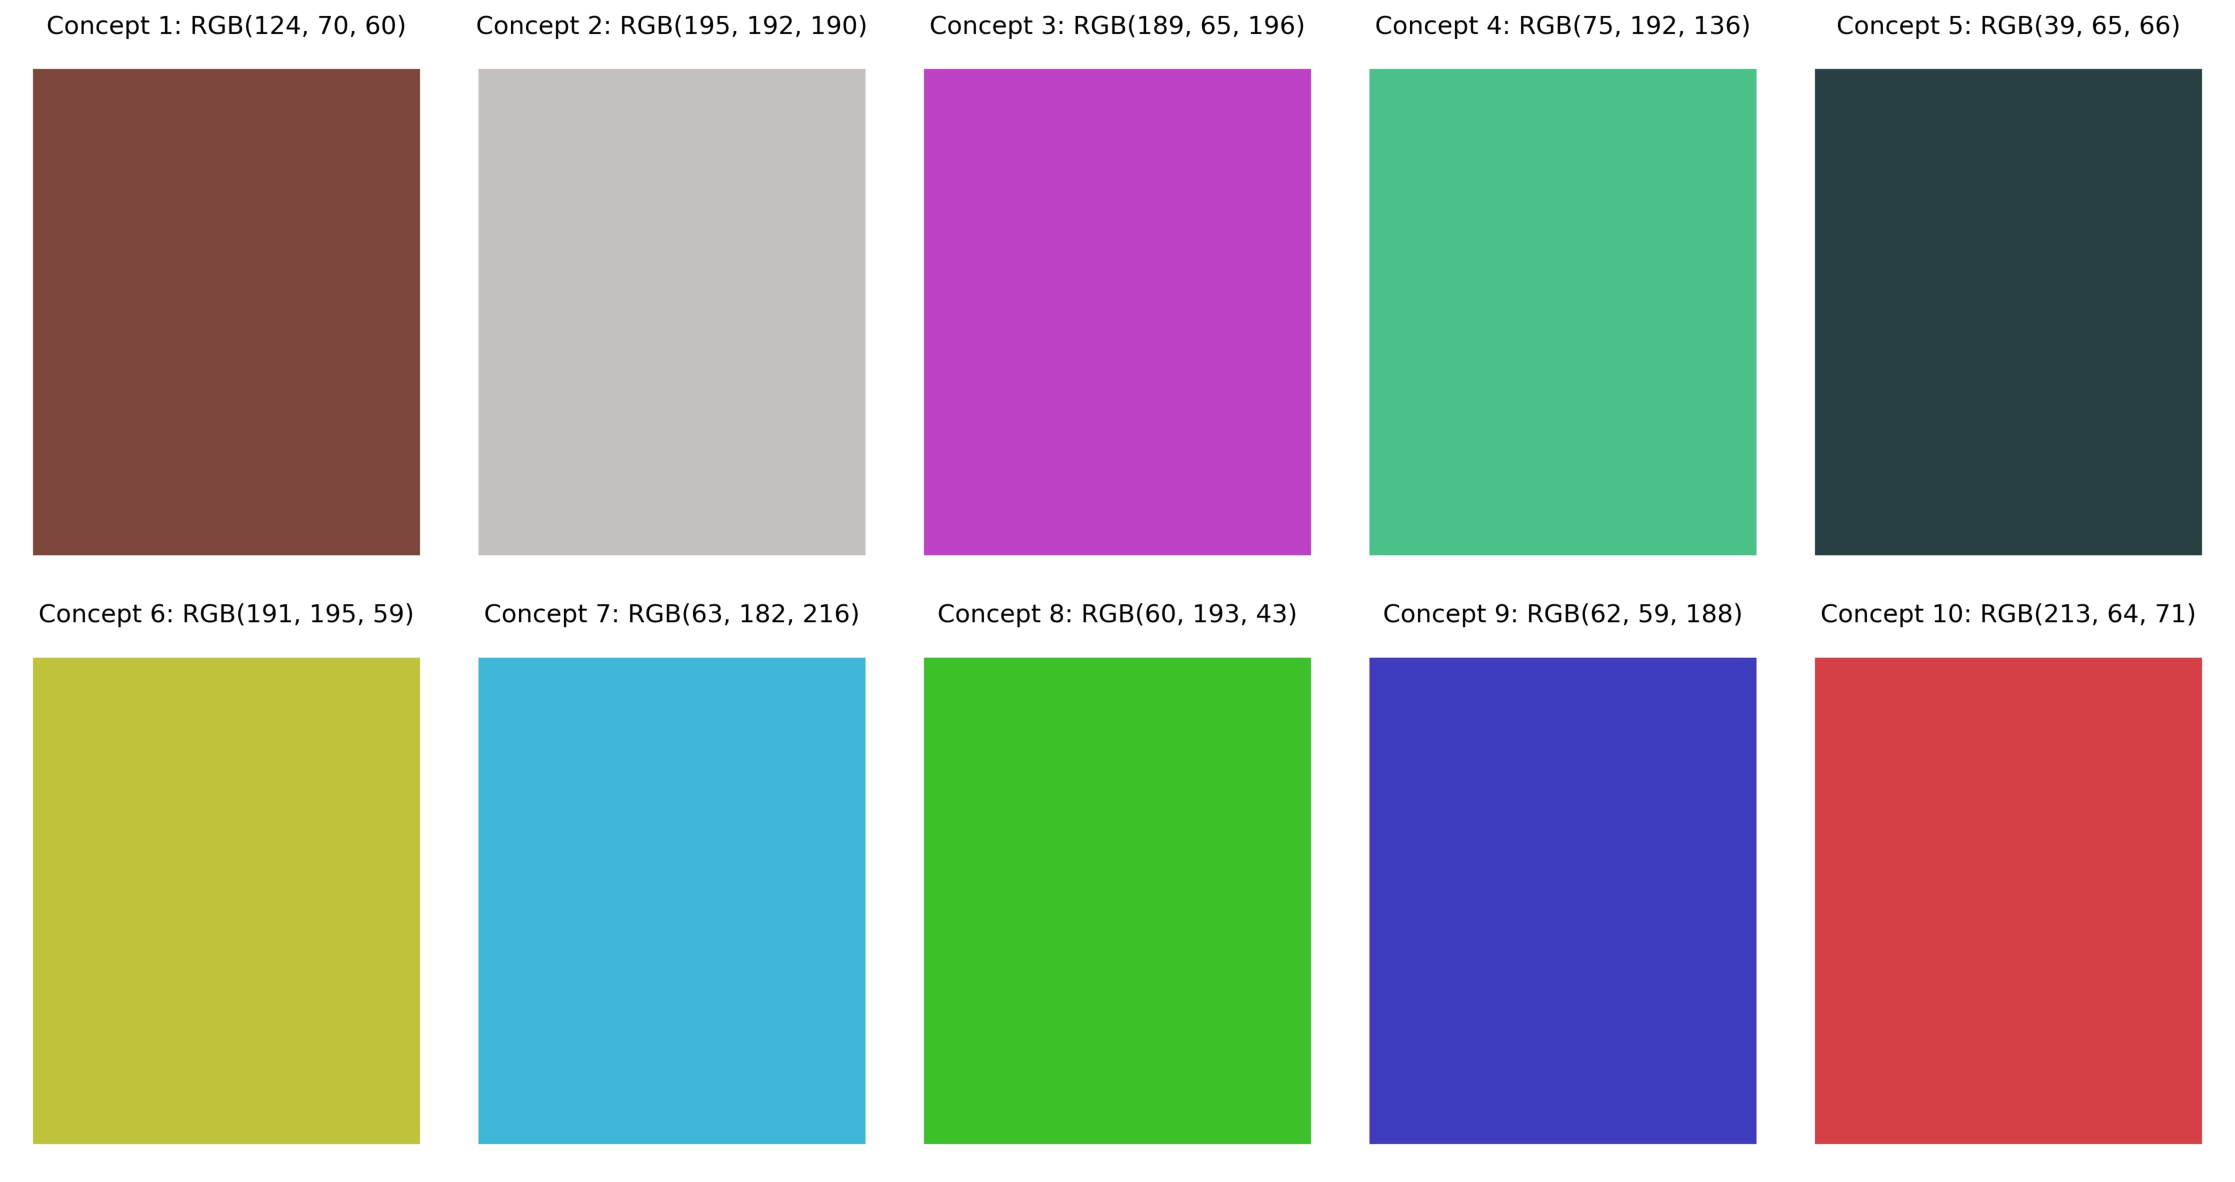
\includegraphics[width=\linewidth]{fig/color_varinace/0.pdf}
    \caption{$\sigma^2 = 0.0$の場合の各色クラスの色の例}
    \label{fig:variance_0}
\end{figure}

\begin{figure}[H]
    \centering
    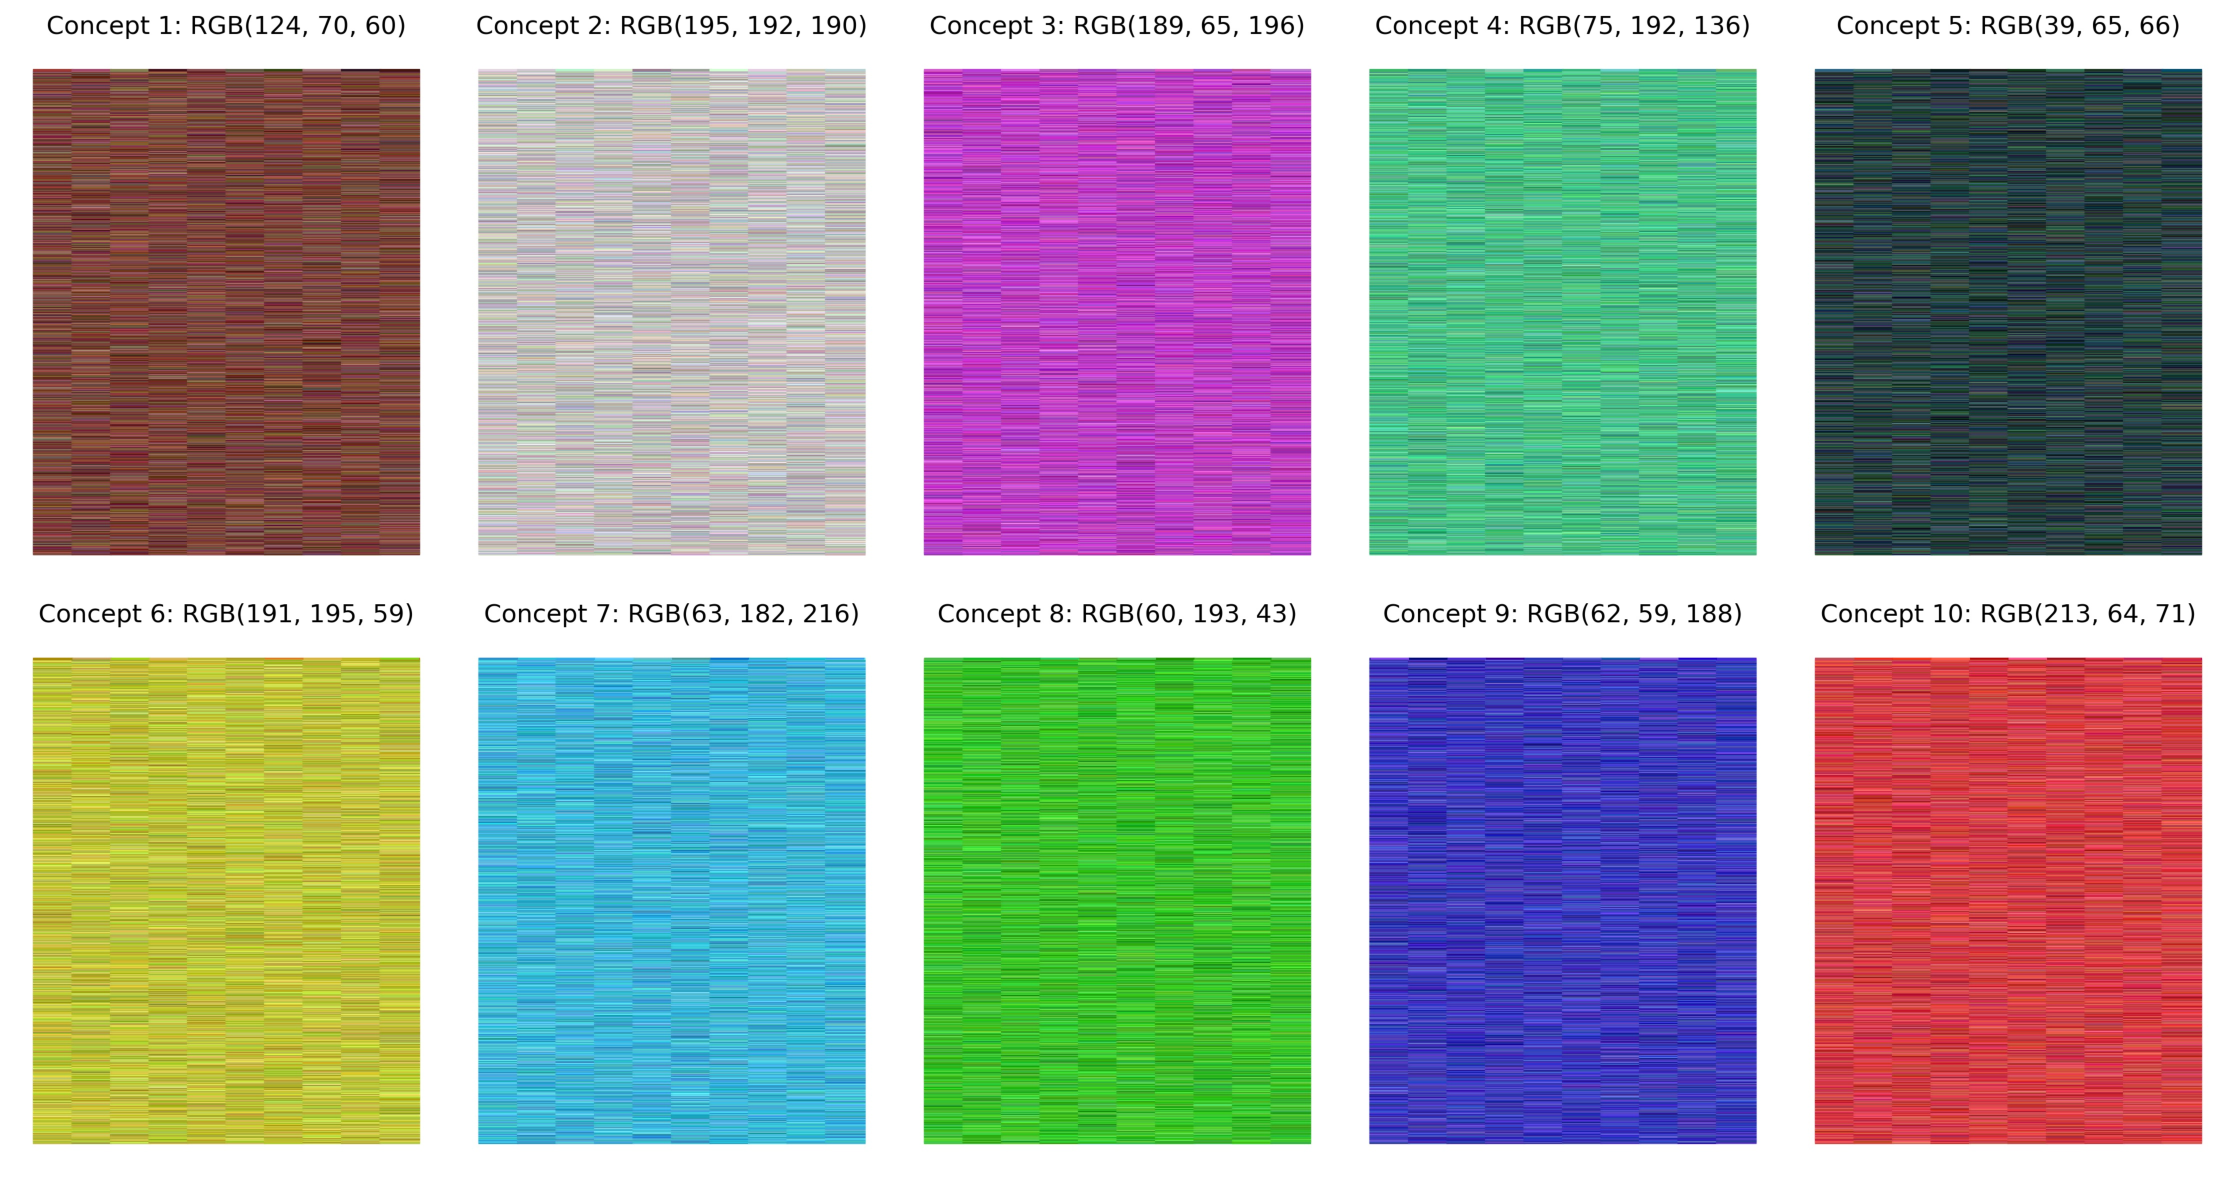
\includegraphics[width=\linewidth]{fig/color_varinace/1000.pdf}
    \caption{$\sigma^2 = 10^3$の場合の各色クラスの色の例}
    \label{fig:variance_1000}
\end{figure}

\begin{figure}[H]
    \centering
    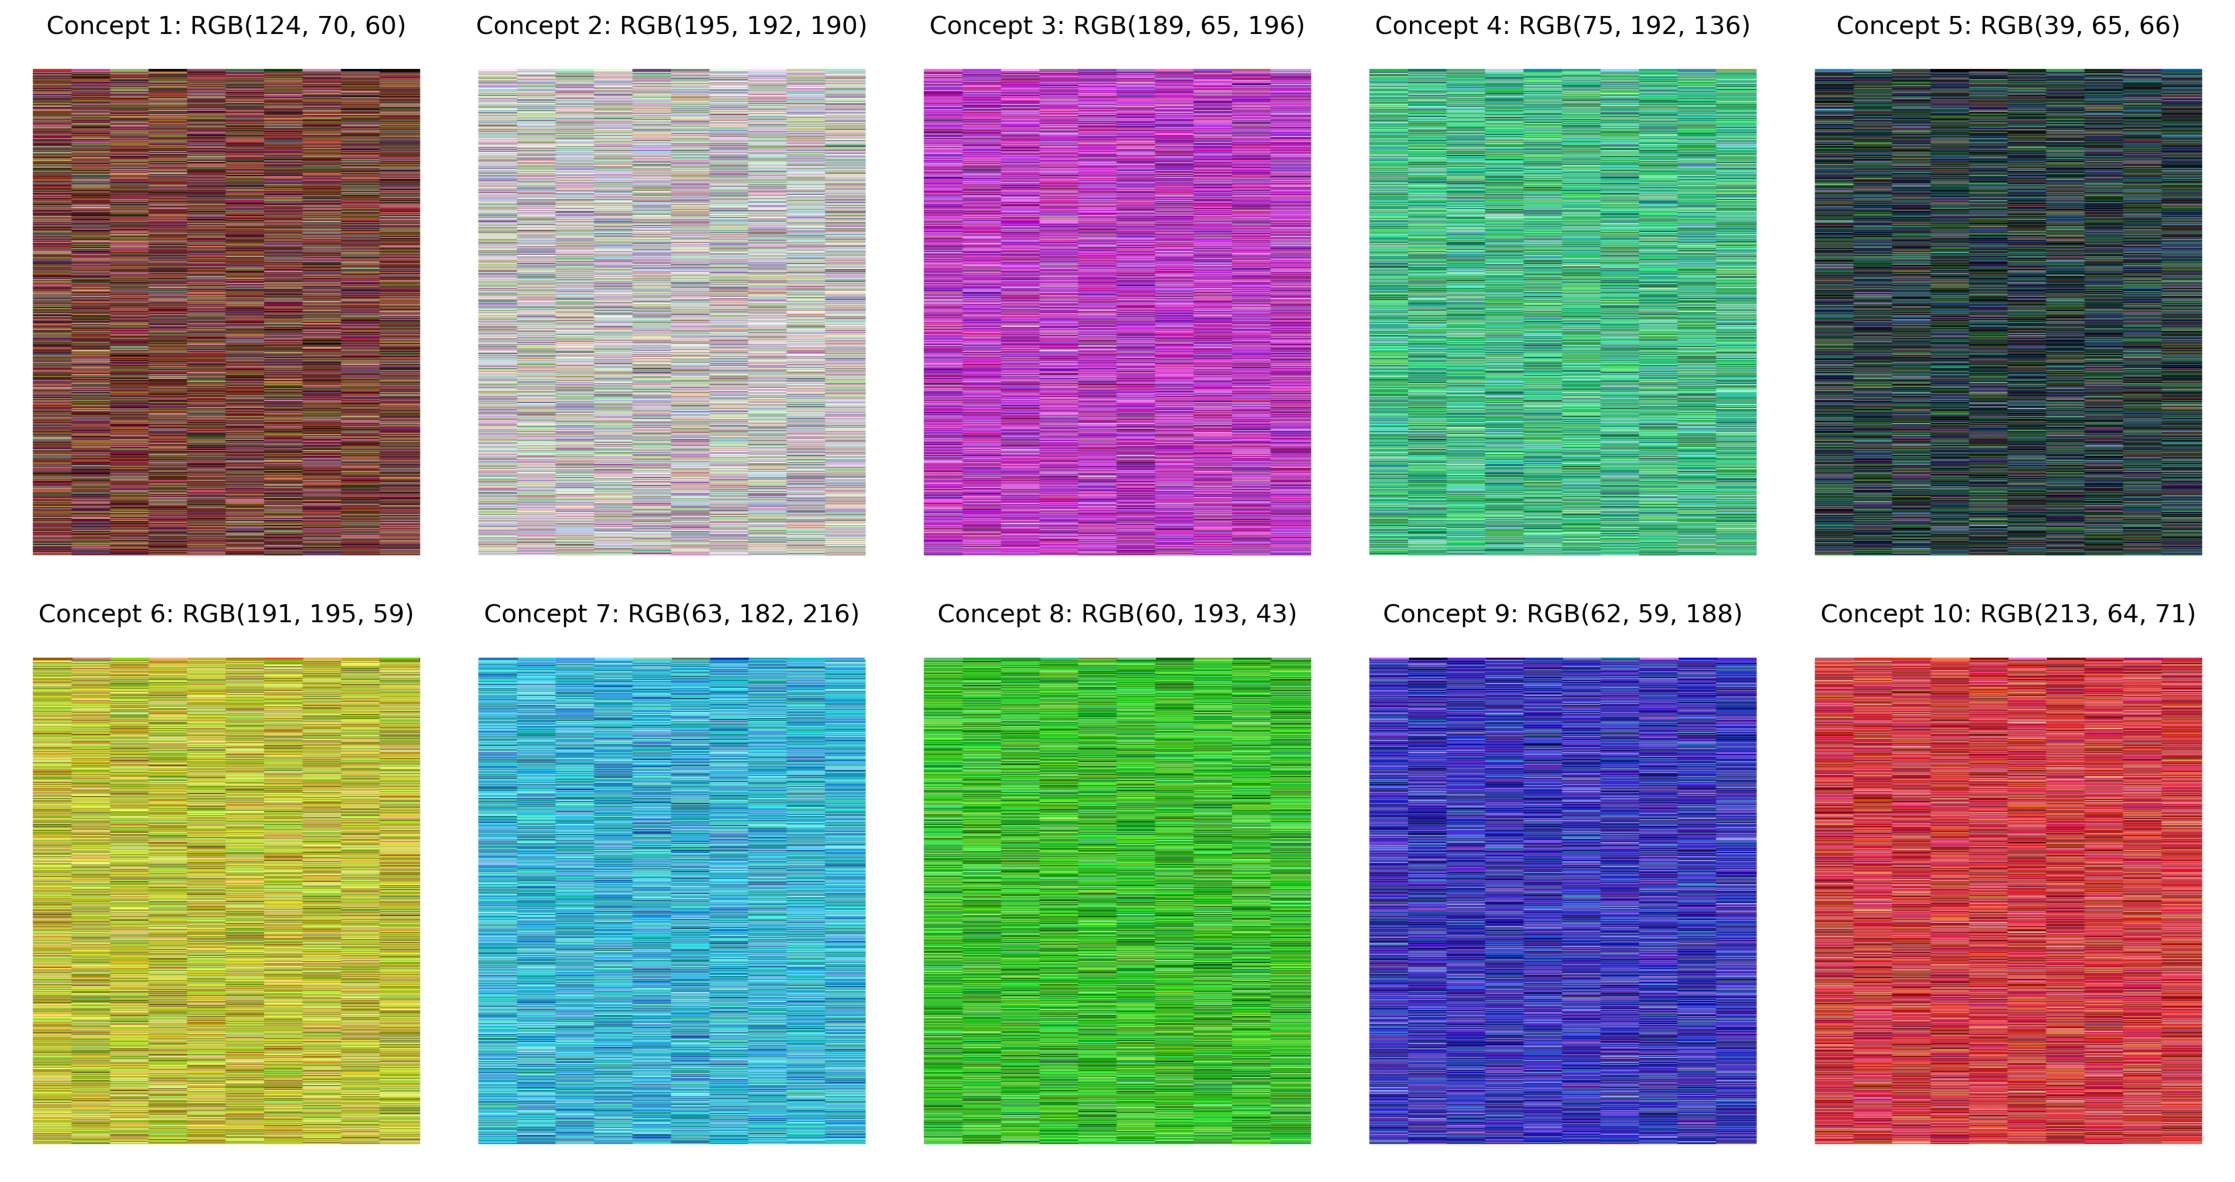
\includegraphics[width=\linewidth]{fig/color_varinace/3612.pdf}
    \caption{$\sigma^2 = 10^{3.5}$の場合の各色クラスの色の例}
    \label{fig:variance_3612}
\end{figure}

\begin{figure}[H]
    \centering
    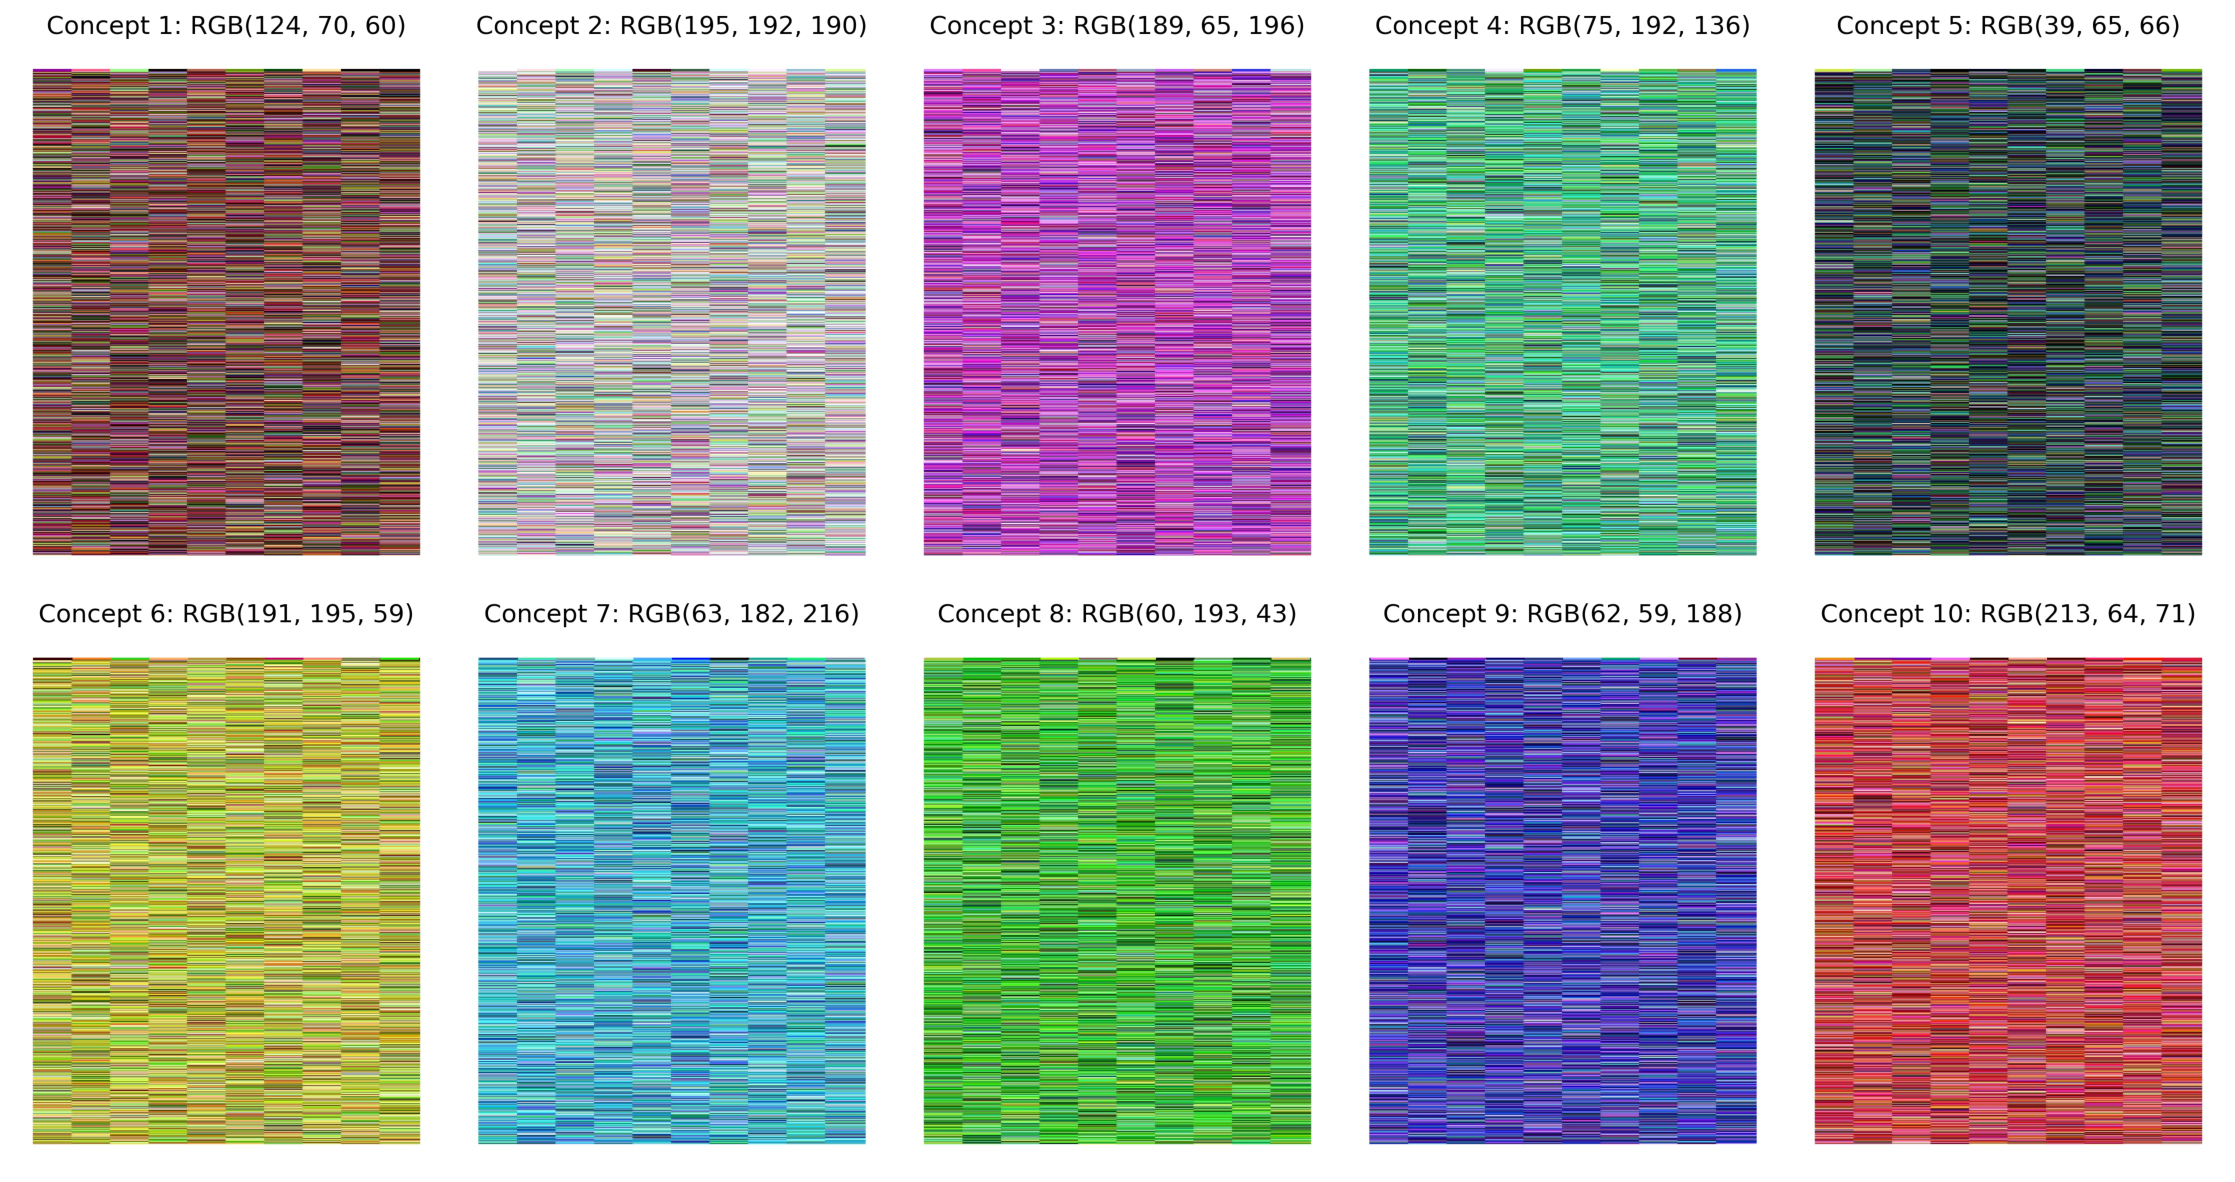
\includegraphics[width=\linewidth]{fig/color_varinace/10000.pdf}
    \caption{$\sigma^2 = 10^4$の場合の各色クラスの色の例}
    \label{fig:variance_10000}
\end{figure}

\begin{figure}[H]
    \centering
    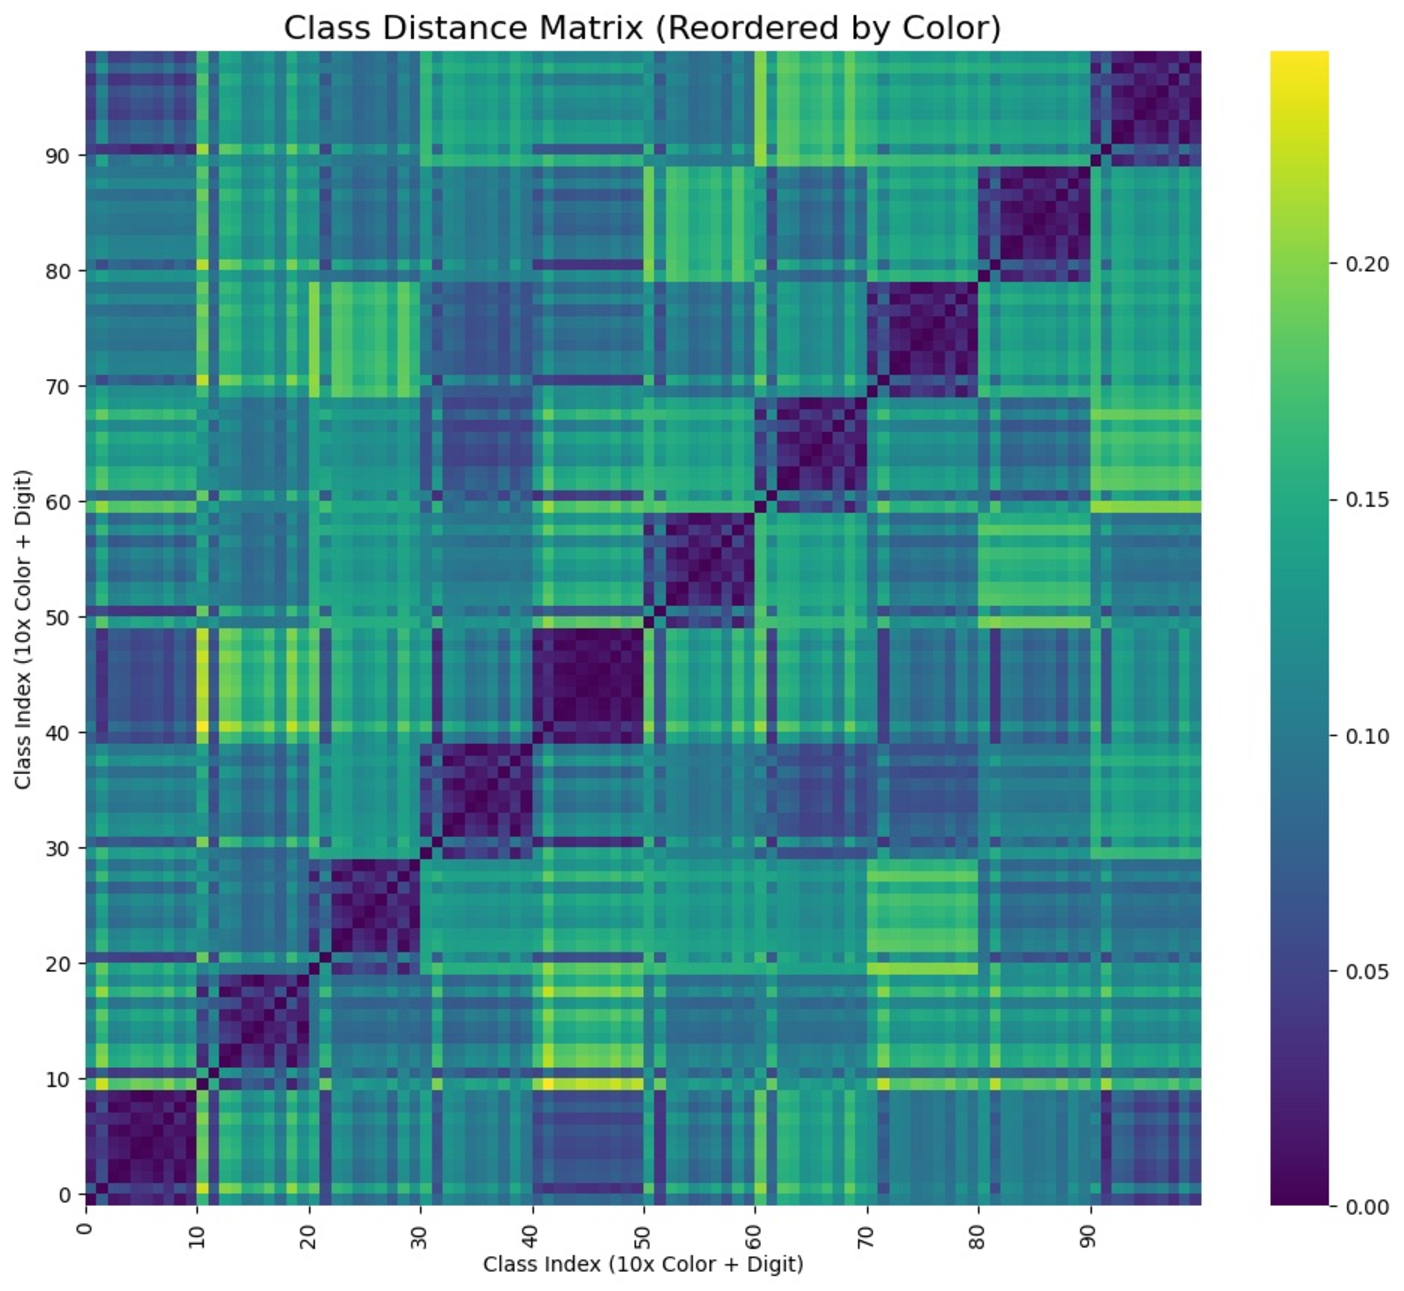
\includegraphics[width=\linewidth]{fig/distance_matrix_heatmap_by_color.pdf}
    \caption{100クラスのクラス間距離のヒートマップ(色,数字順)}
    \label{fig:distance_matrix_heatmap_by_color}
\end{figure}

\begin{figure}[H]
    \centering
    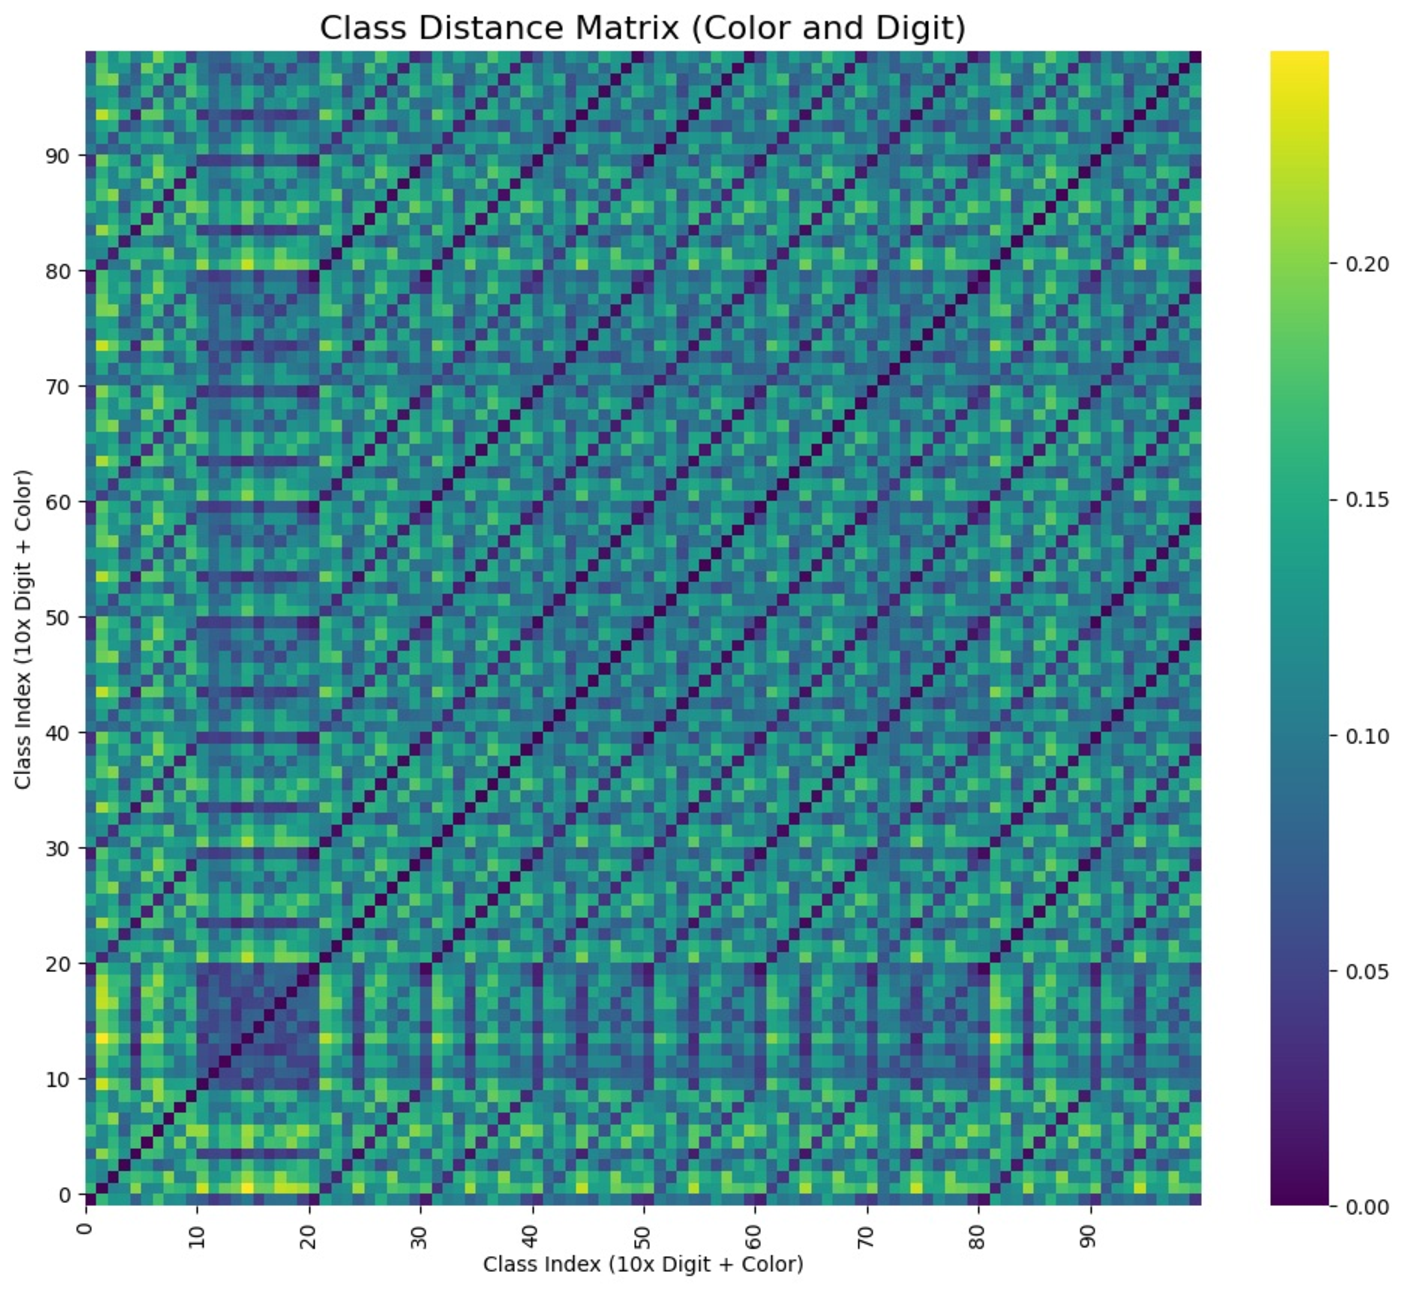
\includegraphics[width=\linewidth]{fig/distance_matrix_heatmap.pdf}
    \caption{100クラスのクラス間距離のヒートマップ(数字,色順)}
    \label{fig:distance_matrix_heatmap_by_digit}
\end{figure}



% % \chapter*{付録}
% \addcontentsline{toc}{chapter}{付録}
\chapter{学習プログラム}
\label{学習プログラム}
学習に利用したプログラムを示す.掲載したプログラムは,GitHub上で公開している.
\\
\url{https://github.com/dsml-lab/double_descent_and_shape_texture_bias}
% カスタムスタイルの定義
\lstdefinestyle{pythonstyle}{
    language=Python,
    basicstyle=\ttfamily\small,
    keywordstyle=\color{blue},
    stringstyle=\color{orange},
    commentstyle=\color{gray}\itshape,
    numbers=left,
    numberstyle=\tiny\color{gray},
    stepnumber=1,
    numbersep=5pt,
    backgroundcolor=\color{lightgray!10},
    frame=single,
    breaklines=true,
    showstringspaces=false,
    captionpos=b
}

\begin{lstlisting}[style=pythonstyle, caption={メインコード}]
    # combineのラベルノイズに関して、色・数字のラベル両方異なるラベルにする
    # accuracyに関して、combineの正解率だけでなく、色・数字の正解率も出力する
    # ラベルノイズの正解率とラベルノイズでない正解率を出力する
    # 平均・分散も出力する
    # 重みの加え方が均等
    
    import os
    import torch
    import torch.nn as nn
    import torch.optim as optim
    import torch.nn.functional as f
    import torch.backends.cudnn as cudnn
    from torch.cuda.amp import autocast, GradScaler
    from torch.utils.data.sampler import Sampler
    import torchvision.transforms as transforms
    from torch.utils.data import DataLoader, TensorDataset
    from sklearn.metrics import classification_report
    from sklearn.metrics import accuracy_score
    import math
    import torchvision.models as models
    import numpy as np
    import time
    import wandb
    import argparse
    import random
    import matplotlib.pyplot as plt
    import csv 
    import warnings
    import gc
    import gzip
    # import models written by scratch
    from model.cnn_2layers import CNN2Layer
    from model.cnn_3layers import CNN3Layer
    from model.cnn_4layers import CNN4Layer
    from model.cnn_5layers import CNN5Layer
    from model.cnn_8layers import CNN8Layer
    from model.cnn_16layers import CNN16Layer
    from model.resnet18 import ResNet18
    # download datasets from pytorch
    from torchvision import datasets
    
    # Ignore warnings
    warnings.filterwarnings("ignore")
    # os.environ['CUDA_LAUNCH_BLOCKING'] = "1"
    # os.environ['PYTORCH_CUDA_ALLOC_CONF'] = 'max_split_size_mb:128'
    torch.backends.cudnn.benchmark = True
    
    # settings
    def parse_args():
        """
        Parse the command-line arguments.
        
        Returns:
            argparse.Namespace: The parsed command-line arguments.
        """
        arg_parser = argparse.ArgumentParser()
        #set seed
        arg_parser.add_argument("-seed", "--fix_seed", type=int, default=42)
        
        #set model settings
        arg_parser.add_argument("--model", type=str, choices=["cnn_2layers", "cnn_3layers", "cnn_4layers", "cnn_5layers", "cnn_8layers", "cnn_16layers", "resnet18"], help="モデルアーキテクチャの選択")
        arg_parser.add_argument("-model_width", "--model_width", type=int, default=1)
        arg_parser.add_argument("-epoch", "--epoch", type=int, default=1000)
        
        #set dataset setting
        arg_parser.add_argument("-datasets", "--dataset", type=str, choices=["mnist", "emnist", "emnist_digits", "cifar10", "cifar100", "tinyImageNet", "colored_emnist", "distribution_colored_emnist"], default="cifar10")
        arg_parser.add_argument("-variance", "--variance", type=int, default=10000)
        arg_parser.add_argument("-correlation", "--correlation", type=float, default=0.5)
        arg_parser.add_argument("-label_noise_rate", "--label_noise_rate", type=float, default=0.0) 
        arg_parser.add_argument("-gray_scale", "--gray_scale", action='store_true', help="グレースケールに変換するかどうか")
        arg_parser.add_argument("-batch_size", "--batch_size", type=int, default=128, help="バッチサイズ")
        arg_parser.add_argument("-img_size", "--img_size", type=int, default=32, help="画像サイズ")
        arg_parser.add_argument("-target", "--target", type=str, choices=["color", "digit", "combined"], default='color', help="colored EMNISTのターゲットの指定:color or digit or combined")
        
        # set optimizer setting
        arg_parser.add_argument("-lr", "--lr", type=float, default=0.1, help="学習率")
        arg_parser.add_argument("-optimizer", "--optimizer", type=str, choices=["sgd", "adam", "adamw", "rmsprop", "adagrad"], default="adam", help="最適化手法.adam were used in Nakkiran et al. (2019)")
        arg_parser.add_argument("-momentum", "--momentum", type=float, default=0.9, help="モーメンタム")
        
        #set loss function setting
        arg_parser.add_argument("-loss", "--loss", type=str, choices=["cross_entropy", "focal_loss"], default="cross_entropy", help="損失関数")
        
        # set device setting
        arg_parser.add_argument("-gpu", "--gpu", type=int, default=0, help="GPU device ID")
        arg_parser.add_argument("-num_workers", "--num_workers", type=int, default=4, help="データローダーの並列数")
        
        # wandb setting
        arg_parser.add_argument("-wandb", "--wandb", action='store_true',default=True ,help="wandbを使用するかどうか")
        arg_parser.add_argument("-wandb_project", "--wandb_project", type=str, default="dd_scratch_models", help="wandbのプロジェクト名")
        arg_parser.add_argument("--wandb_entity", type=str, default="dsml-kernel24", help="wandbのエンティティ名")
        
        
        arg_parser.add_argument("-weight_noisy", "--weight_noisy", type=float, default=1.0, help="Weight for the loss of noisy samples")
        arg_parser.add_argument("-weight_clean", "--weight_clean", type=float, default=1.0, help="Weight for the loss of clean samples")
        return arg_parser.parse_args()
    
    # Define a custom dataset that includes noise_info
    class NoisyDataset(torch.utils.data.Dataset):
        def __init__(self, dataset, noise_info):
            self.dataset = dataset
            self.noise_info = noise_info
    
        def __len__(self):
            return len(self.dataset)
    
        def __getitem__(self, idx):
            input, label = self.dataset[idx]
            noise_label = self.noise_info[idx]
            return input, label, noise_label
    
    # Custom sampler to create balanced batches
    class BalancedBatchSampler(Sampler):
        def __init__(self, clean_indices, noisy_indices, batch_size, drop_last):
            self.clean_indices = clean_indices
            self.noisy_indices = noisy_indices
            self.batch_size = batch_size
            self.drop_last = drop_last
    
            assert batch_size % 2 == 0, "Batch size must be even for balanced batches"
            self.num_samples_per_class = batch_size // 2
    
        def __iter__(self):
            # Shuffle the indices
            random.shuffle(self.clean_indices)
            random.shuffle(self.noisy_indices)
    
            # Calculate the number of batches
            min_len = min(len(self.clean_indices), len(self.noisy_indices))
            num_batches = min_len // self.num_samples_per_class
    
            for i in range(num_batches):
                clean_batch = self.clean_indices[i * self.num_samples_per_class: (i + 1) * self.num_samples_per_class]
                noisy_batch = self.noisy_indices[i * self.num_samples_per_class: (i + 1) * self.num_samples_per_class]
                batch = clean_batch + noisy_batch
                random.shuffle(batch)
                yield batch
    
            if not self.drop_last:
                # Handle remaining samples
                remaining_clean = self.clean_indices[num_batches * self.num_samples_per_class:]
                remaining_noisy = self.noisy_indices[num_batches * self.num_samples_per_class:]
    
                if len(remaining_clean) >= self.num_samples_per_class and len(remaining_noisy) >= self.num_samples_per_class:
                    batch = remaining_clean[:self.num_samples_per_class] + remaining_noisy[:self.num_samples_per_class]
                    random.shuffle(batch)
                    yield batch
    
        def __len__(self):
            return len(self.clean_indices) // self.num_samples_per_class
    
    # Set seeds
    def set_seed(seed):
        """
        Set the seed for reproducibility.
    
        Args:
            seed (int): The seed value to set.
    
        Returns:
            None
        """
        random.seed(seed)
        np.random.seed(seed)
        torch.manual_seed(seed)
        torch.cuda.manual_seed(seed)
        torch.cuda.manual_seed_all(seed)
        # For GPU determinism
        torch.backends.cudnn.deterministic = True
        torch.backends.cudnn.benchmark = False
    
    # Set device
    def set_device(gpu_id):
        """
        Sets the device for computation.
    
        Args:
            gpu_id (int): The ID of the GPU to use.
    
        Returns:
            torch.device: The selected device (GPU or CPU).
        """
        # Choose the GPU device if available, otherwise use CPU
        device = torch.device("cuda:{}".format(gpu_id) if torch.cuda.is_available() else "cpu")
        return device
    
    def clear_memory():
        torch.cuda.empty_cache()  # Clear CUDA cache
        gc.collect()  # Force garbage collection
    
    def apply_transform(x, transform):
        transformed_x = []
        for img in x:
            img = transform(img)
            transformed_x.append(img)
        return torch.stack(transformed_x)
    
    def load_datasets(dataset, target, gray_scale, args):
        """
        Load the specified dataset and apply transformations based on the dataset type and grayscale option.
        
        Args:
            dataset (str): The name of the dataset to load. Supported options are "mnist", "emnist", "cifar10", "cifar100", and "tinyImageNet".
            gray_scale (bool): Flag indicating whether to convert the images to grayscale.
            
        Returns:
            tuple: A tuple containing the train dataset, test dataset, image size, and number of classes.
        """
        if dataset == "mnist":
            transform = transforms.Compose([
                transforms.ToTensor(),
                transforms.Resize((32, 32)),
                transforms.Normalize((0.1307,), (0.3081,))
            ])
            train_dataset = datasets.MNIST(root='./data', train=True, download=True, transform=transform)
            test_dataset = datasets.MNIST(root='./data', train=False, download=True, transform=transform)
            imagesize = (32, 32)
            num_classes = 10
            in_channels = 1
        elif dataset == "emnist":
            transform = transforms.Compose([
                transforms.ToTensor(),
                transforms.Resize((32, 32)),
                transforms.Normalize((0.1307,), (0.3081,))
            ])
            train_dataset = datasets.EMNIST(root='./data', split='balanced', train=True, download=True, transform=transform)
            test_dataset = datasets.EMNIST(root='./data', split='balanced', train=False, download=True, transform=transform)
            imagesize = (32, 32)
            num_classes = 47
            in_channels = 1
        elif dataset == "emnist_digits":
            emnist_path = './data/EMNIST'
            def load_gz_file(file_path, is_image=True):
                with gzip.open(file_path, 'rb') as f:
                    if is_image:
                        return np.frombuffer(f.read(), dtype=np.uint8, offset=16).reshape(-1, 28, 28)
                    else:
                        return np.frombuffer(f.read(), dtype=np.uint8, offset=8)
    
            x_train = load_gz_file(os.path.join(emnist_path, 'emnist-digits-train-images-idx3-ubyte.gz'))
            y_train = load_gz_file(os.path.join(emnist_path, 'emnist-digits-train-labels-idx1-ubyte.gz'), is_image=False)
            x_test = load_gz_file(os.path.join(emnist_path, 'emnist-digits-test-images-idx3-ubyte.gz'))
            y_test = load_gz_file(os.path.join(emnist_path, 'emnist-digits-test-labels-idx1-ubyte.gz'), is_image=False)
            # 変換関数が必要な場合はここで定義
            transform = transforms.Compose([
                transforms.ToPILImage(),  # Convert numpy array to PIL Image
                transforms.Resize((32, 32)),  # Same size as original, adjust if needed
                transforms.ToTensor()
            ])
    
            # Apply transformation
            x_train_tensor = apply_transform(x_train, transform)
            x_test_tensor = apply_transform(x_test, transform)
    
            y_train_tensor = torch.tensor(y_train, dtype=torch.long)
            y_test_tensor = torch.tensor(y_test, dtype=torch.long)
    
            train_dataset = torch.utils.data.TensorDataset(x_train_tensor, y_train_tensor)
            test_dataset = torch.utils.data.TensorDataset(x_test_tensor, y_test_tensor)
    
            num_classes = 10  # Digits from 0 to 9
            in_channels = 1  # Grayscale images
            imagesize = (32, 32)  # Original image size
        elif dataset == "colored_emnist":
            # target: color or digit or combined
            
            # Data augmentation
            transform = transforms.Compose([
                transforms.ToPILImage(),  # Convert numpy array to PIL Image
                transforms.Resize((32, 32)),
                transforms.ToTensor(),
                transforms.Normalize((0.1307,), (0.3081,))
            ])
            
            if target == 'color':
                x_train = np.load('data/colored_EMNIST/x_train_colored.npy')
                y_train_colors = np.load('data/colored_EMNIST/y_train_colors.npy')
                x_test = np.load('data/colored_EMNIST/x_test_colored.npy')
                y_test_colors = np.load('data/colored_EMNIST/y_test_colors.npy')
                
                # Apply transformation
                x_train_tensor = apply_transform(x_train, transform)
                x_test_tensor = apply_transform(x_test, transform)
                
                y_train_tensor = torch.tensor(y_train_colors, dtype=torch.long)
                y_test_tensor = torch.tensor(y_test_colors, dtype=torch.long)
                
                train_dataset = torch.utils.data.TensorDataset(x_train_tensor, y_train_tensor)
                test_dataset = torch.utils.data.TensorDataset(x_test_tensor, y_test_tensor)
            
            elif target == 'digit':
                x_train = np.load('data/colored_EMNIST/x_train_colored.npy')
                y_train_digits = np.load('data/colored_EMNIST/y_train_digits.npy')
                x_test = np.load('data/colored_EMNIST/x_test_colored.npy')
                y_test_digits = np.load('data/colored_EMNIST/y_test_digits.npy')
                
                # Apply transformation
                x_train_tensor = apply_transform(x_train, transform)
                x_test_tensor = apply_transform(x_test, transform)
                
                y_train_tensor = torch.tensor(y_train_digits, dtype=torch.long)
                y_test_tensor = torch.tensor(y_test_digits, dtype=torch.long)
                
                train_dataset = torch.utils.data.TensorDataset(x_train_tensor, y_train_tensor)
                test_dataset = torch.utils.data.TensorDataset(x_test_tensor, y_test_tensor)
                
            elif target == 'combined':
                x_train = np.load('data/colored_EMNIST/x_train_colored.npy')
                y_train_combined = np.load('data/colored_EMNIST/y_train_combined.npy')
                x_test = np.load('data/colored_EMNIST/x_test_colored.npy')
                y_test_combined = np.load('data/colored_EMNIST/y_test_combined.npy')
                
                # Apply transformation
                x_train_tensor = apply_transform(x_train, transform)
                x_test_tensor = apply_transform(x_test, transform)
                
                y_train_tensor = torch.tensor(y_train_combined, dtype=torch.long)
                y_test_tensor = torch.tensor(y_test_combined, dtype=torch.long)
                
                train_dataset = torch.utils.data.TensorDataset(x_train_tensor, y_train_tensor)
                test_dataset = torch.utils.data.TensorDataset(x_test_tensor, y_test_tensor)
                
            num_classes = 10 if target in ['color', 'digit'] else 100
            in_channels = 3
            imagesize = (32, 32)
        elif dataset == "distribution_colored_emnist":
            # target: color or digit or combined
            seed = args.fix_seed
            variance = args.variance
            correlation = args.correlation
            # Data augmentation
            transform = transforms.Compose([
                transforms.ToPILImage(),  # Convert numpy array to PIL Image
                transforms.Resize((32, 32)),
                transforms.ToTensor(),
                transforms.Normalize((0.1307,), (0.3081,))
            ])
            
            if target == 'color':
                x_train = np.load(f'data/distribution_colored_EMNIST_Seed42_Var{variance}_Corr{correlation}/x_train_colored.npy')
                y_train_colors = np.load(f'data/distribution_colored_EMNIST_Seed42_Var{variance}_Corr{correlation}/y_train_colors.npy')
                x_test = np.load(f'data/distribution_colored_EMNIST_Seed42_Var{variance}_Corr{correlation}/x_test_colored.npy')
                y_test_colors = np.load(f'data/distribution_colored_EMNIST_Seed42_Var{variance}_Corr{correlation}/y_test_colors.npy')
                
                # Apply transformation
                x_train_tensor = apply_transform(x_train, transform)
                x_test_tensor = apply_transform(x_test, transform)
                
                y_train_tensor = torch.tensor(y_train_colors, dtype=torch.long)
                y_test_tensor = torch.tensor(y_test_colors, dtype=torch.long)
                
                train_dataset = torch.utils.data.TensorDataset(x_train_tensor, y_train_tensor)
                test_dataset = torch.utils.data.TensorDataset(x_test_tensor, y_test_tensor)
            
            elif target == 'digit':
                x_train = np.load(f'data/distribution_colored_EMNIST_Seed42_Var{variance}_Corr{correlation}/x_train_colored.npy')
                y_train_digits = np.load(f'data/distribution_colored_EMNIST_Seed42_Var{variance}_Corr{correlation}/y_train_digits.npy')
                x_test = np.load(f'data/distribution_colored_EMNIST_Seed42_Var{variance}_Corr{correlation}/x_test_colored.npy')
                y_test_digits = np.load(f'data/distribution_colored_EMNIST_Seed42_Var{variance}_Corr{correlation}/y_test_digits.npy')
                
                # Apply transformation
                x_train_tensor = apply_transform(x_train, transform)
                x_test_tensor = apply_transform(x_test, transform)
                
                y_train_tensor = torch.tensor(y_train_digits, dtype=torch.long)
                y_test_tensor = torch.tensor(y_test_digits, dtype=torch.long)
                
                train_dataset = torch.utils.data.TensorDataset(x_train_tensor, y_train_tensor)
                test_dataset = torch.utils.data.TensorDataset(x_test_tensor, y_test_tensor)
                
            elif target == 'combined':
                x_train = np.load(f'data/distribution_colored_EMNIST_Seed42_Var{variance}_Corr{correlation}/x_train_colored.npy')
                y_train_combined = np.load(f'data/distribution_colored_EMNIST_Seed42_Var{variance}_Corr{correlation}/y_train_combined.npy')
                x_test = np.load(f'data/distribution_colored_EMNIST_Seed42_Var{variance}_Corr{correlation}/x_test_colored.npy')
                y_test_combined = np.load(f'data/distribution_colored_EMNIST_Seed42_Var{variance}_Corr{correlation}/y_test_combined.npy')
                
                # Apply transformation
                x_train_tensor = apply_transform(x_train, transform)
                x_test_tensor = apply_transform(x_test, transform)
                
                y_train_tensor = torch.tensor(y_train_combined, dtype=torch.long)
                y_test_tensor = torch.tensor(y_test_combined, dtype=torch.long)
                
                train_dataset = torch.utils.data.TensorDataset(x_train_tensor, y_train_tensor)
                test_dataset = torch.utils.data.TensorDataset(x_test_tensor, y_test_tensor)
        
            num_classes = 10 if target in ['color', 'digit'] else 100
            in_channels = 3
            imagesize = (32, 32)
        elif dataset == "cifar10":
            transform = transforms.Compose([
                transforms.RandomCrop(32, padding=4),
                transforms.RandomHorizontalFlip(),
                transforms.ToTensor(),
                transforms.Normalize((0.4914, 0.4822, 0.4465), (0.2023, 0.1994, 0.2010))
            ])
            train_dataset = datasets.CIFAR10(root='./data', train=True, download=True, transform=transform)
            test_dataset = datasets.CIFAR10(root='./data', train=False, download=True, transform=transform)
            imagesize = (32, 32)
            num_classes = 10
            in_channels = 3
        elif dataset == "cifar100":
            transform = transforms.Compose([
                transforms.RandomCrop(32, padding=4),
                transforms.RandomHorizontalFlip(),
                transforms.ToTensor(),
                transforms.Normalize((0.5071, 0.4867, 0.4408), (0.2675, 0.2565, 0.2761))
            ])
            train_dataset = datasets.CIFAR100(root='./data', train=True, download=True, transform=transform)
            test_dataset = datasets.CIFAR100(root='./data', train=False, download=True, transform=transform)
            imagesize = (32, 32)
            num_classes = 100
            in_channels = 3
        elif dataset == "tinyImageNet":
            transform = transforms.Compose([
                transforms.RandomCrop(64, padding=4),
                transforms.RandomHorizontalFlip(),
                transforms.ToTensor(),
                transforms.Normalize((0.4802, 0.4481, 0.3975), (0.2302, 0.2265, 0.2262))
            ])
            train_dataset = datasets.ImageFolder(root='./data/tiny-imagenet-200/train', transform=transform)
            test_dataset = datasets.ImageFolder(root='./data/tiny-imagenet-200/val', transform=transform)
            imagesize = (64, 64)
            num_classes = 200
            in_channels = 3
        elif dataset == "distribution_to_normal":
            # target: color or digit or combined
            seed = args.fix_seed
            variance = args.variance
            correlation = args.correlation
            # Data augmentation
            transform = transforms.Compose([
                transforms.ToPILImage(),  # Convert numpy array to PIL Image
                transforms.Resize((32, 32)),
                transforms.ToTensor(),
                transforms.Normalize((0.1307,), (0.3081,))
            ])
            if target == 'combined':
                x_train = np.load(f'data/distribution_colored_EMNIST_Seed42_Var{variance}_Corr{correlation}/x_train_colored.npy')
                y_train_combined = np.load(f'data/distribution_colored_EMNIST_Seed42_Var{variance}_Corr{correlation}/y_train_combined.npy')
                x_test = np.load('data/colored_EMNIST/x_test_colored.npy')
                y_test_combined = np.load('data/colored_EMNIST/y_test_combined.npy')
                
                # Apply transformation
                x_train_tensor = apply_transform(x_train, transform)
                x_test_tensor = apply_transform(x_test, transform)
                
                y_train_tensor = torch.tensor(y_train_combined, dtype=torch.long)
                y_test_tensor = torch.tensor(y_test_combined, dtype=torch.long)
                
                train_dataset = torch.utils.data.TensorDataset(x_train_tensor, y_train_tensor)
                test_dataset = torch.utils.data.TensorDataset(x_test_tensor, y_test_tensor)
        
            num_classes = 10 if target in ['color', 'digit'] else 100
            in_channels = 3
            imagesize = (32, 32)
        else:
            raise ValueError("Invalid dataset name")
            
    
        if gray_scale:
            transform = transforms.Compose([
                transforms.Grayscale(),
                transforms.ToTensor(),
                transforms.Normalize((0.1307,), (0.3081,))
            ])
            train_dataset.transform = transform
            test_dataset.transform = transform  
    
        return train_dataset, test_dataset, imagesize, num_classes, in_channels
    
    def load_models(in_channels, args, img_size, num_classes):
        if args.model == "cnn_2layers":
            model = CNN2Layer(in_channels, num_classes, args.model_width, img_size)
        elif args.model == "cnn_3layers":
            model = CNN3Layer(in_channels, num_classes, args.model_width, img_size)
        elif args.model == "cnn_4layers":
            model = CNN4Layer(in_channels, num_classes, args.model_width, img_size)
        elif args.model == "cnn_5layers":
            model = CNN5Layer(in_channels, num_classes, args.model_width, img_size)
        elif args.model == "cnn_8layers":
            model = CNN8Layer(in_channels, num_classes, args.model_width, img_size)
        elif args.model == "cnn_16layers":
            model = CNN16Layer(in_channels, num_classes, args.model_width, img_size)
        elif args.model == "resnet18":
            model = models.resnet18(num_classes=num_classes)
        else:
            raise ValueError("Invalid model name.")
        return model
    
    # Modify add_label_noise to return indices of noisy samples
    def add_label_noise(targets, label_noise_rate, num_digits, num_colors):
        noisy_targets = targets.clone()
        num_noisy = int(label_noise_rate * len(targets))
        noisy_indices = torch.randperm(len(targets))[:num_noisy]
        noise_info = torch.zeros(len(targets), dtype=torch.int)  # Initialize as clean
    
        if num_digits == 10 and num_colors == 1:
            for idx in noisy_indices:
                original_label = targets[idx].item()
                new_label = random.randint(0, num_digits - 1)
                while new_label == original_label:
                    new_label = random.randint(0, num_digits - 1)
                noisy_targets[idx] = new_label
                noise_info[idx] = 1  # Mark as noisy
    
        elif num_digits == 10 and num_colors == 10:
            for idx in noisy_indices:
                original_label = targets[idx].item()
                original_digit = original_label // num_colors
                original_color = original_label % num_colors
    
                new_digit = random.randint(0, num_digits - 1)
                new_color = random.randint(0, num_colors - 1)
                new_label = new_digit * num_colors + new_color
                while new_label == original_label:
                    new_digit = random.randint(0, num_digits - 1)
                    new_color = random.randint(0, num_colors - 1)
                    new_label = new_digit * num_colors + new_color
    
                noisy_targets[idx] = new_label
                noise_info[idx] = 1  # Mark as noisy
    
        return noisy_targets, noise_info
    
    def train_model(model, train_loader, optimizer, criterion, weight_noisy, weight_clean, device, num_colors, num_digits):
        """
        Training function with comprehensive metrics tracking.
        
        Args:
            model: The neural network model
            train_loader: DataLoader for training data
            optimizer: The optimizer
            criterion: Loss function (expected to support reduction='none')
            weight_noisy: Weight for noisy samples
            weight_clean: Weight for clean samples
            device: Device to run the training on
            num_colors: Number of color classes
            num_digits: Number of digit classes
            
        Returns:
            dict: Dictionary containing all training metrics
        """
        model.train()
        running_loss = 0.0
        total_samples = 0
        correct_total = 0
    
        # Initialize counters for noisy and clean samples
        correct_noisy = 0
        total_noisy = 0
        correct_clean = 0
        total_clean = 0
    
        # Initialize counters for digits and colors
        correct_digit_total = 0
        correct_color_total = 0
    
        correct_digit_noisy = 0
        correct_color_noisy = 0
        correct_digit_clean = 0
        correct_color_clean = 0
    
        # Lists for loss tracking
        loss_values = []
        loss_values_noisy = []
        loss_values_clean = []
    
        # Ensure criterion returns per-sample losses
        criterion.reduction = 'none'
    
        for inputs, labels, noise_labels in train_loader:
            try:
                # Move data to device
                inputs = inputs.to(device, non_blocking=True)
                labels = labels.to(device, non_blocking=True)
                noise_labels = noise_labels.to(device, non_blocking=True)
    
                # Zero the parameter gradients
                optimizer.zero_grad()
    
                # Forward pass
                outputs = model(inputs)
                _, predicted = torch.max(outputs.data, 1)
                
                # Calculate batch size and update total samples
                batch_size = labels.size(0)
                total_samples += batch_size
    
                # Get indices for noisy and clean samples
                idx_noisy = (noise_labels == 1)
                idx_clean = (noise_labels == 0)
    
                # Count noisy and clean samples in batch
                num_noisy = idx_noisy.sum().item()
                num_clean = idx_clean.sum().item()
    
                # Compute per-sample losses
                per_sample_loss = criterion(outputs, labels)
    
                # Calculate weights for the batch
                total_weight = weight_clean + weight_noisy
                weights = torch.zeros_like(per_sample_loss, device=device)
                
                if num_noisy == 0:  # All clean samples
                    weights = torch.ones_like(per_sample_loss, device=device) * (weight_clean / total_weight) * 2
                elif num_clean == 0:  # All noisy samples
                    weights = torch.ones_like(per_sample_loss, device=device) * (weight_noisy / total_weight) * 2
                else:  # Mixed batch
                    weights[idx_noisy] = (weight_noisy / total_weight) * 2
                    weights[idx_clean] = (weight_clean / total_weight) * 2
    
                # Apply weights to losses
                per_sample_loss_weighted = per_sample_loss * weights
    
                # Compute mean loss and backpropagate
                loss = per_sample_loss_weighted.mean()
                loss.backward()
                optimizer.step()
    
                # Update running loss and total accuracy
                running_loss += loss.item() * batch_size
                correct_total += (predicted == labels).sum().item()
    
                digit_labels = labels // num_colors
                color_labels = labels % num_colors
                digit_predictions = predicted // num_colors
                color_predictions = predicted % num_colors
    
                correct_digit_total += (digit_predictions == digit_labels).sum().item()
                correct_color_total += (color_predictions == color_labels).sum().item()
    
                # Process noisy samples
                if num_noisy > 0:
                    labels_noisy = labels[idx_noisy]
                    predicted_noisy = predicted[idx_noisy]
                    correct_noisy += (predicted_noisy == labels_noisy).sum().item()
                    total_noisy += num_noisy
    
                    # Update digit and color accuracy for noisy samples
                    digit_labels_noisy = labels_noisy // num_colors
                    color_labels_noisy = labels_noisy % num_colors
                    digit_predictions_noisy = predicted_noisy // num_colors
                    color_predictions_noisy = predicted_noisy % num_colors
    
                    correct_digit_noisy += (digit_predictions_noisy == digit_labels_noisy).sum().item()
                    correct_color_noisy += (color_predictions_noisy == color_labels_noisy).sum().item()
    
                    # Store noisy sample losses
                    loss_values_noisy.extend(per_sample_loss_weighted[idx_noisy].detach().cpu().numpy())
    
                # Process clean samples
                if num_clean > 0:
                    labels_clean = labels[idx_clean]
                    predicted_clean = predicted[idx_clean]
                    correct_clean += (predicted_clean == labels_clean).sum().item()
                    total_clean += num_clean
    
                    # Update digit and color accuracy for clean samples
                    digit_labels_clean = labels_clean // num_colors
                    color_labels_clean = labels_clean % num_colors
                    digit_predictions_clean = predicted_clean // num_colors
                    color_predictions_clean = predicted_clean % num_colors
    
                    correct_digit_clean += (digit_predictions_clean == digit_labels_clean).sum().item()
                    correct_color_clean += (color_predictions_clean == color_labels_clean).sum().item()
    
                    # Store clean sample losses
                    loss_values_clean.extend(per_sample_loss_weighted[idx_clean].detach().cpu().numpy())
    
                # Store all losses
                loss_values.extend(per_sample_loss_weighted.detach().cpu().numpy())
    
            except Exception as e:
                print(f"Error in training batch: {str(e)}")
                continue
    
        # Calculate loss statistics
        avg_loss = np.mean(loss_values) if loss_values else float('nan')
        var_loss = np.var(loss_values) if loss_values else float('nan')
    
        avg_loss_noisy = np.mean(loss_values_noisy) if loss_values_noisy else float('nan')
        var_loss_noisy = np.var(loss_values_noisy) if loss_values_noisy else float('nan')
    
        avg_loss_clean = np.mean(loss_values_clean) if loss_values_clean else float('nan')
        var_loss_clean = np.var(loss_values_clean) if loss_values_clean else float('nan')
    
        # Calculate accuracies
        metrics = {
            'avg_loss': avg_loss,
            'var_loss': var_loss,
            'accuracy_total': 100. * correct_total / total_samples if total_samples > 0 else float('nan'),
            'accuracy_noisy': 100. * correct_noisy / total_noisy if total_noisy > 0 else float('nan'),
            'accuracy_clean': 100. * correct_clean / total_clean if total_clean > 0 else float('nan'),
            'avg_loss_noisy': avg_loss_noisy,
            'var_loss_noisy': var_loss_noisy,
            'avg_loss_clean': avg_loss_clean,
            'var_loss_clean': var_loss_clean,
            'accuracy_digit_total': 100. * correct_digit_total / total_samples if total_samples > 0 else float('nan'),
            'accuracy_color_total': 100. * correct_color_total / total_samples if total_samples > 0 else float('nan'),
            'accuracy_digit_noisy': 100. * correct_digit_noisy / total_noisy if total_noisy > 0 else float('nan'),
            'accuracy_color_noisy': 100. * correct_color_noisy / total_noisy if total_noisy > 0 else float('nan'),
            'accuracy_digit_clean': 100. * correct_digit_clean / total_clean if total_clean > 0 else float('nan'),
            'accuracy_color_clean': 100. * correct_color_clean / total_clean if total_clean > 0 else float('nan'),
            'total_samples': total_samples,
            'total_noisy': total_noisy,
            'total_clean': total_clean,
            'correct_total': correct_total,
            'correct_noisy': correct_noisy,
            'correct_clean': correct_clean
        }
    
        return metrics
    
    def test_model(model, test_loader, device, num_colors, num_digits):
        model.eval()
        loss_values = []  # 損失値を保存するリスト
        test_loss = 0
        correct_total = 0
        total_samples = 0
    
        correct_digit_total = 0
        correct_color_total = 0
    
        # criterion を 'none' に設定して個々のサンプルの損失を取得
        criterion = nn.CrossEntropyLoss(reduction='none')
    
        with torch.no_grad():
            for inputs, labels in test_loader:
                inputs, labels = inputs.to(device), labels.to(device)
                outputs = model(inputs)
                
                # 個々のサンプルの損失を計算
                per_sample_loss = criterion(outputs, labels)
                loss_values.extend(per_sample_loss.cpu().numpy())
                
                # バッチ全体の損失を計算
                test_loss += per_sample_loss.mean().item() * labels.size(0)
                
                _, predicted = torch.max(outputs, 1)
                total_samples += labels.size(0)
                correct_total += (predicted == labels).sum().item()
    
                # Calculate correct counts for digits and colors
                digit_labels = labels // num_colors
                color_labels = labels % num_colors
                digit_predictions = predicted // num_colors
                color_predictions = predicted % num_colors
    
                correct_digit_total += (digit_predictions == digit_labels).sum().item()
                correct_color_total += (color_predictions == color_labels).sum().item()
    
        # 損失の平均と分散を計算
        avg_loss = test_loss / total_samples if total_samples > 0 else float('nan')
        var_loss = np.var(loss_values) if loss_values else float('nan')
        
        accuracy_total = 100. * correct_total / total_samples if total_samples > 0 else float('nan')
        accuracy_digit_total = 100. * correct_digit_total / total_samples if total_samples > 0 else float('nan')
        accuracy_color_total = 100. * correct_color_total / total_samples if total_samples > 0 else float('nan')
    
        return {
            'avg_loss': avg_loss,
            'var_loss': var_loss,  # 追加
            'accuracy_total': accuracy_total,
            'accuracy_digit_total': accuracy_digit_total,
            'accuracy_color_total': accuracy_color_total,
            'total_samples': total_samples,
            'correct_total': correct_total
        }
        
    def main():
        """
        Main training loop with comprehensive error handling and logging
        """
        print('Start session')
        wandb_run = None
        
        try:
            # Parse arguments and set initial configurations
            args = parse_args()
            set_seed(args.fix_seed)
            
            # Set device
            device = set_device(args.gpu)
            print(f'Using device: {device}')
    
            # Load datasets with error handling
            print('Loading datasets...')
            try:
                train_dataset, test_dataset, imagesize, num_classes, in_channels = load_datasets(
                    args.dataset, args.target, args.gray_scale, args)
            except FileNotFoundError as e:
                print(f"Error loading dataset: {e}")
                return
            except Exception as e:
                print(f"Unexpected error loading dataset: {e}")
                return
    
            # Set number of digit and color classes
            if args.target == 'combined':
                num_digits = 10
                num_colors = 10
            else:
                num_digits = 10
                num_colors = 1
    
            # Add label noise and create NoisyDataset
            print(f'Preparing dataset with label noise rate: {args.label_noise_rate}')
            if args.label_noise_rate > 0.0:
                if hasattr(train_dataset, 'tensors'):
                    x_train, y_train = train_dataset.tensors
                    y_train_noisy, noise_info = add_label_noise(y_train, args.label_noise_rate, num_digits, num_colors)
                    train_dataset = torch.utils.data.TensorDataset(x_train, y_train_noisy)
                    train_dataset = NoisyDataset(train_dataset, noise_info)
                else:
                    y_train = torch.tensor(train_dataset.targets)
                    y_train_noisy, noise_info = add_label_noise(y_train, args.label_noise_rate, num_digits, num_colors)
                    train_dataset.targets = y_train_noisy.tolist()
                    train_dataset = NoisyDataset(train_dataset, noise_info)
            else:
                noise_info = torch.zeros(len(train_dataset), dtype=torch.int)
                train_dataset = NoisyDataset(train_dataset, noise_info)
    
            # Extract indices for clean and noisy samples
            clean_indices = [i for i, label in enumerate(noise_info) if label == 0]
            noisy_indices = [i for i, label in enumerate(noise_info) if label == 1]
    
            # Validate batch size
            if args.batch_size % 2 != 0:
                raise ValueError("Batch size must be even for balanced batches")
    
            # Create data loaders
            print('Setting up data loaders...')
            if args.label_noise_rate == 0.0 or args.label_noise_rate == 1.0:
                train_loader = torch.utils.data.DataLoader(
                    train_dataset,
                    batch_size=args.batch_size,
                    shuffle=True,
                    num_workers=args.num_workers,
                    pin_memory=True
                )
            else:
                batch_sampler = BalancedBatchSampler(
                    clean_indices,
                    noisy_indices,
                    args.batch_size,
                    drop_last=False
                )
                train_loader = torch.utils.data.DataLoader(
                    train_dataset,
                    batch_sampler=batch_sampler,
                    num_workers=args.num_workers,
                    pin_memory=True
                )
    
            test_loader = torch.utils.data.DataLoader(
                test_dataset,
                batch_size=args.batch_size,
                shuffle=False,
                num_workers=args.num_workers,
                pin_memory=True
            )
    
            # Initialize model
            print('Initializing model...')
            model = load_models(in_channels, args, imagesize, num_classes)
            model = model.to(device)
    
            # Set optimizer
            print('Setting up optimizer...')
            if args.optimizer == "sgd":
                optimizer = optim.SGD(model.parameters(), lr=args.lr, momentum=args.momentum)
            elif args.optimizer == "adam":
                optimizer = optim.Adam(model.parameters(), lr=args.lr)
            elif args.optimizer == "adamw":
                optimizer = optim.AdamW(model.parameters(), lr=args.lr)
            elif args.optimizer == "rmsprop":
                optimizer = optim.RMSprop(model.parameters(), lr=args.lr, momentum=args.momentum)
            elif args.optimizer == "adagrad":
                optimizer = optim.Adagrad(model.parameters(), lr=args.lr)
            else:
                raise ValueError(f"Unsupported optimizer: {args.optimizer}")
    
            # Set loss function
            criterion = nn.CrossEntropyLoss(reduction='none')
    
            # Set experiment name
            experiment_name = (
                f'{args.model}_{args.dataset}_{args.target}_'
                f'lr{args.lr}_batch{args.batch_size}_epoch{args.epoch}_'
                f'LabelNoiseRate{args.label_noise_rate}_Optim{args.optimizer}_'
                f'cleanw{args.weight_clean}_noisew{args.weight_noisy}_variance{args.variance}_width{args.model_width}_'
                f'seed{args.fix_seed}'
                
            )
            print(f'Experiment name: {experiment_name}')
    
            # Initialize wandb
            if args.wandb:
                print('Initializing wandb...')
                wandb_run = wandb.init(
                    project=args.wandb_project,
                    name=experiment_name,
                    entity=args.wandb_entity,
                    config=args
                )
    
            # Set up CSV logging
            csv_dir = f"./csv/combine/split_noise/{experiment_name}"
            os.makedirs(csv_dir, exist_ok=True)
            csv_path = os.path.join(csv_dir, 'log.csv')
            
            if not os.path.isfile(csv_path):
                with open(csv_path, 'w', newline='') as f:
                    writer = csv.writer(f)
                    writer.writerow([
                        "epoch", 
                        "train_loss", "train_loss_variance",
                        "train_accuracy", "train_accuracy_noisy", "train_accuracy_clean",
                        "train_accuracy_digit_total", "train_accuracy_color_total",
                        "train_accuracy_digit_noisy", "train_accuracy_color_noisy",
                        "train_accuracy_digit_clean", "train_accuracy_color_clean",
                        "test_loss", "test_loss_variance",
                        "test_accuracy",
                        "test_accuracy_digit_total", "test_accuracy_color_total"
                    ])
    
            # Training loop
            print('Starting training...')
            best_test_accuracy = 0.0
            for epoch in range(1, args.epoch + 1):
                try:
                    # Training phase
                    train_metrics = train_model(
                        model=model,
                        train_loader=train_loader,
                        optimizer=optimizer,
                        criterion=criterion,
                        weight_noisy=args.weight_noisy,
                        weight_clean=args.weight_clean,
                        device=device,
                        num_colors=num_colors,
                        num_digits=num_digits
                    )
    
                    # Testing phase
                    test_metrics = test_model(
                        model=model,
                        test_loader=test_loader,
                        device=device,
                        num_colors=num_colors,
                        num_digits=num_digits
                    )
    
                    # Print progress
                    print(f"\nEpoch: {epoch}/{args.epoch}")
                    print(f"Train Loss: {train_metrics['avg_loss']:.4f}, "
                          f"Train Loss Variance: {train_metrics['var_loss']:.4f}")
                    print(f"Train Accuracy: {train_metrics['accuracy_total']:.2f}%, "
                          f"Test Accuracy: {test_metrics['accuracy_total']:.2f}%")
                    print(f"Train Digit/Color Accuracy: {train_metrics['accuracy_digit_total']:.2f}%/"
                          f"{train_metrics['accuracy_color_total']:.2f}%")
                    print(f"Test Digit/Color Accuracy: {test_metrics['accuracy_digit_total']:.2f}%/"
                          f"{test_metrics['accuracy_color_total']:.2f}%")
    
                    # Save to CSV
                    with open(csv_path, 'a', newline='') as f:
                        writer = csv.writer(f)
                        writer.writerow([
                            epoch,
                            train_metrics['avg_loss'], train_metrics['var_loss'],
                            train_metrics['accuracy_total'],
                            train_metrics['accuracy_noisy'],
                            train_metrics['accuracy_clean'],
                            train_metrics['accuracy_digit_total'],
                            train_metrics['accuracy_color_total'],
                            train_metrics['accuracy_digit_noisy'],
                            train_metrics['accuracy_color_noisy'],
                            train_metrics['accuracy_digit_clean'],
                            train_metrics['accuracy_color_clean'],
                            test_metrics['avg_loss'], test_metrics['var_loss'],
                            test_metrics['accuracy_total'],
                            test_metrics['accuracy_digit_total'],
                            test_metrics['accuracy_color_total']
                        ])
    
                    # Log to wandb
                    if args.wandb:
                        wandb.log({
                            'epoch': epoch,
                            'train_loss': train_metrics['avg_loss'],
                            'train_loss_variance': train_metrics['var_loss'],
                            'train_accuracy': train_metrics['accuracy_total'],
                            'train_accuracy_noisy': train_metrics['accuracy_noisy'],
                            'train_accuracy_clean': train_metrics['accuracy_clean'],
                            'train_accuracy_digit_total': train_metrics['accuracy_digit_total'],
                            'train_accuracy_color_total': train_metrics['accuracy_color_total'],
                            'train_accuracy_digit_noisy': train_metrics['accuracy_digit_noisy'],
                            'train_accuracy_color_noisy': train_metrics['accuracy_color_noisy'],
                            'train_accuracy_digit_clean': train_metrics['accuracy_digit_clean'],
                            'train_accuracy_color_clean': train_metrics['accuracy_color_clean'],
                            'test_loss': test_metrics['avg_loss'],
                            'test_loss_variance': test_metrics['var_loss'],
                            'test_accuracy': test_metrics['accuracy_total'],
                            'test_accuracy_digit_total': test_metrics['accuracy_digit_total'],
                            'test_accuracy_color_total': test_metrics['accuracy_color_total']
                        })
    
                    # Memory management
                    if epoch % 10 == 0:
                        clear_memory()
    
                    # Save best model
                    if test_metrics['accuracy_total'] > best_test_accuracy:
                        best_test_accuracy = test_metrics['accuracy_total']
                        torch.save(model.state_dict(), 
                                 os.path.join(csv_dir, 'best_model.pth'))
    
                except Exception as e:
                    print(f"Error in epoch {epoch}: {str(e)}")
                    continue
    
        except Exception as e:
            print(f"Fatal error in training: {str(e)}")
            raise
        
        finally:
            # Cleanup
            if wandb_run is not None:
                wandb_run.finish()
            print('Training completed')
    
    if __name__ == '__main__':
        main()
\end{lstlisting}


% \chapter{対外成果発表リスト}
\begin{enumerate}
    \item[2022-04-16] 出場チーム名 MIT, AIイノベーションアワード2022, 開催地 立教大学, \\AI企業賞(https://www.nttpc.co.jp/press/2022/04/202204211500.html).
    \item[2024-08-06] \underline{岩瀬 俊}, 平本 麗弥,前田 英作, ``CNNのの学習過程における概念獲得について
,''  第27回 画像の認識・理解シンポジウム(MIRU2024), IS-1-050, ポスター発表, 開催地 熊本城ホール(熊本県).
    \item[2024-11-29]  \underline{岩瀬 俊},平本麗弥,前田英作, ``CNNの学習過程における概念獲得について
,''  パターン認識・メディア理解(PRMU)2024月11月研究会, PRMU2024-15, 口頭発表(査読なし), 福井工業大学(福井県).
    \item[2024-12-05] \underline{Shun Iwase},Shuya Takahashi,Nakamasa Inoue,Rio Yokota,Ryo Nakamura,Hirokatsu Kataoka,Eisaku Maeda, ``On the Relationship Between Double Descent of CNNs and Shape/Texture Bias Under LearningProcess
,''  International Conference on Pattern Recognition(ICPR), 20245, 口頭発表(査読あり), Biswa Bangla Convention Centre(インド・コルカタ).

\end{enumerate}


\bibliographystyle{IEEEtran}
\bibliography{ref/mybibfile.bib}

\end{document}